\documentclass[10pt,openany]{article}
\usepackage{ctex} 
\usepackage{geometry,graphicx,xcolor,color}
\geometry{
	a4paper,
	top=25.4mm, bottom=25.4mm,
	left=20mm, right=20mm,
	headheight=2.17cm,
	headsep=4mm,
	footskip=12mm
}
\usepackage[all,pdf]{xy}
\usepackage{amssymb,amsmath,mathrsfs}             
\usepackage{mathpazo}
\usepackage[nofontspec]{newpxtext}
\usepackage{array}
\usepackage{amsmath}
\usepackage{amssymb}
\usepackage{enumerate}
\usepackage{amsthm}
\usepackage{bm}
\usepackage{mathtools}
\usepackage{mathrsfs}
\usepackage{tcolorbox}
\usepackage{indentfirst}
\usepackage{setspace}
\usepackage{subfigure} 
\usepackage{tkz-fct}
\usetikzlibrary{calc,intersections,through,backgrounds,3d}
\usetikzlibrary{shapes,arrows}
\tikzstyle{startstop} = [rectangle,rounded corners, minimum width=3cm,minimum height=1cm,draw=black,fill=red!30]
\tikzstyle{io} = [trapezium, trapezium left angle = 70,trapezium right angle=110,minimum width=3cm,minimum height=1cm,text centered,draw=black,fill=blue!30]
\tikzstyle{process} = [rectangle,minimum width=4cm,minimum height=1cm,text centered,text width =4cm,draw=black,fill=red!30]
\tikzstyle{decision} = [diamond,minimum width=3cm,minimum height=1cm,text centered,draw=black,fill=green!30]
\tikzstyle{arrow} = [thick,->,>=stealth]

\usepackage{tkz-euclide}
\usepackage{tikz-3dplot}
\usepackage{pgfplots}
\usepackage{booktabs}
\usepackage{float}
\usepackage[graphicx]{realboxes}
\usepackage{fancyhdr}
\usepackage{nicematrix}
\definecolor{winered}{rgb}{0.5,0,0}
\definecolor{structurecolor}{RGB}{122,122,142}
\definecolor{main}{HTML}{3D445F}
\definecolor{second}{HTML}{627581}
\definecolor{third}{HTML}{333333}
\definecolor{deepgreen}{HTML}{2F5E4E}  
\definecolor{purple}{HTML}{512E5F}   

\usepackage{hyperref}
\hypersetup{colorlinks = true, linktoc=all, linkcolor=blue, urlcolor=winered}


\usepackage{amsthm}
\usepackage{xcolor}
\usepackage{etoolbox}
\newtheoremstyle{defstyle}
{0.3cm}{0.3cm}{\fangsong}{-1cm}{\bfseries\color{main}}{}{0.5em}
{\indent 【\thmname{#1} \thmnumber{#2}】\ifthenelse{\equal{#3}{}}{}{~\thmnote{(#3)}}}

\newtheoremstyle{thmstyle}
{0.3cm}{0.3cm}{\kaishu}{-1cm}{\bfseries\color{second}}{}{0.5em}
{\indent 【\thmname{#1} \thmnumber{#2}】\ifthenelse{\equal{#3}{}}{}{~\thmnote{(#3)}}}

\newtheoremstyle{remstyle}
{0.3cm}{0.3cm}{\kaishu}{-1cm}{\bfseries\color{third}}{}{0.5em}
{\indent 【\thmname{#1} \thmnumber{#2}】\ifthenelse{\equal{#3}{}}{}{~\thmnote{(#3)}}}

\newtheoremstyle{exastyle}
{0.3cm}{0.3cm}{\kaishu}{-1cm}{\bfseries\color{deepgreen}}{}{0.5em}
{\indent 【\thmname{#1} \thmnumber{#2}】\ifthenelse{\equal{#3}{}}{}{~\thmnote{(#3)}}}

\newtheoremstyle{prostyle}
{0.3cm}{0.3cm}{\kaishu}{-1cm}{\bfseries\color{purple}}{}{0.5em}
{\indent 【\thmname{#1} \thmnumber{#2}】\ifthenelse{\equal{#3}{}}{}{~\thmnote{(#3)}}}

\theoremstyle{thmstyle} %theorem style
\newtheorem{theorem}{定理}[subsection]
\newtheorem{practice}{练习}[section]
\theoremstyle{defstyle} % definition style
\newtheorem{definition}[theorem]{定义}
\newtheorem{defprop}[theorem]{定义\(-\)命题}
\newtheorem{lemma}[theorem]{引理}
\newtheorem{corollary}[theorem]{推论}
\theoremstyle{prostyle} % proposition style
\newtheorem{proposition}[theorem]{命题}
\newtheorem{property}[theorem]{性质}
\theoremstyle{exastyle} 
\newtheorem{example}[theorem]{例}
\AtEndEnvironment{example}{\hfill \( \diamondsuit \)}
\theoremstyle{remstyle} 
\newtheorem{remark}[theorem]{注}

\renewenvironment{proof}[1][证明]{\par\underline{\textbf{#1.}} \;\fangsong}{\qed\par}
\newenvironment{solution}{\par\underline{\textbf{解.}} \;\fangsong}{\qed\par}
\newcommand{\intro}[1]{\rightline{\parbox[t]{5cm}{\footnotesize \fangsong\quad\quad #1 }}}

\AtEndEnvironment{proof}{\vspace{1.5ex}}
\AtEndEnvironment{solution}{\vspace{1.5ex}}

\usepackage{titlesec, titletoc}
\linespread{1.2} 				
\usepackage{fancyhdr}
\fancyhf{}
\renewcommand{\headrule}{\color{structurecolor}\hrule width\textwidth}
\pagestyle{fancy}
\renewcommand{\headrulewidth}{1pt}
\fancypagestyle{plain}{\renewcommand{\headrulewidth}{0pt}\fancyhf{}\renewcommand{\headrule}{}}

\fancyhead[c]{\color{structurecolor}\kaishu\rightmark}
\fancyfoot[c]{\color{structurecolor}\small\thepage}


\titleformat{\section}[frame]{\normalfont\color{structurecolor}}{\footnotesize \enspace \large \textcolor{structurecolor}{\S \,\thesection}\enspace}{6pt}{\Large\filcenter \bf \kaishu }


\titleformat{\subsection}[hang]{\bfseries}{\large\bfseries\color{structurecolor}\thesubsection\enspace}{1pt}{\color{structurecolor}\large\bfseries\filright}

\titleformat{\subsubsection}[hang]{\bfseries}{\large\bfseries\color{structurecolor}\thesubsubsection\enspace}{1pt}{\color{structurecolor}\large\bfseries\filright}

\usepackage{titling}
\renewcommand*{\maketitle}{
	\begin{titlepage}
		\newgeometry{margin = 0in}
		\parindent=0pt
		\includegraphics[width=\linewidth]{cover.png}
		\vfill
		\begin{center}
			\parbox{0.618\textwidth}{
				\hfill {\bfseries \Huge \thetitle} \\[0.6pt]  
				\rule{0.618\textwidth}{4pt} \\ 
			}
		\end{center}
		\vfill
		\begin{center}
			\parbox{0.618\textwidth}{
				\hfill\Large
				\kaishu 
				\begin{tabular}{r|}
					\textbf{2025 Summer} \\
					作者:\theauthor \\ 
					时间:\thedate \\
				\end{tabular}
			}
		\end{center}
		\vfill
		\begin{center}
			\parbox[t]{0.7\textwidth}{\centering \kaishu}
		\end{center}
		\vfill
	\end{titlepage}
	\restoregeometry
	\thispagestyle{empty}
}

\newcommand{\T}{^{\text{T}}}
\newcommand{\Her}{^{\text{H}}}
\newcommand{\F}{\mathbb{F}}
\newcommand{\gfn}{\text{GL}_n(\mathbb{F})}
\newcommand{\gfm}{\text{GL}_m(\mathbb{F})}
\newcommand{\C}{\mathbb{C}}
\newcommand{\R}{\mathbb{R}}
\newcommand{\Q}{\mathbb{Q}}
\newcommand{\n}{^{n \times n}}
\newcommand{\mn}{^{m \times n}}
\newcommand{\nm}{^{n \times m}}
\newcommand{\leinv}{_\text{L}^{-1}}
\newcommand{\riinv}{_\text{R}^{-1}}
\newcommand{\tz}{\mathrm{char} \;} 
\newcommand{\tr}{\mathrm{tr}}
\newcommand{\diag}{\mathrm{diag}}
\newcommand{\bmxi}{\bm{\xi}}
\newcommand{\bmeta}{\bm{\eta}}
\newcommand{\bme}{\bm{e}}
\newcommand{\oneb}{\underline{\hspace{1em}}\hspace{0.001em}}
\newcommand{\twob}{\oneb\oneb}
\newcommand{\fourb}{\twob\twob}
\newcommand{\tenb}{\twob\twob\twob\twob\twob}
\newcommand{\tideparallel}{%  
	\mathrel{%  
		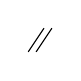
\begin{tikzpicture}[scale=0.2, baseline={([yshift=-0.5ex]current bounding box.center)}]  
			\draw[thin] (0,0) -- (1,1.5);  
			\draw[thin] (0.5,0) -- (1.5,1.5);  
		\end{tikzpicture}%  
	}%  
}  
\newcommand{\fourch}[4]
{\\[3pt]
	\begin{tabular}
		{*{4}{@{}p{4cm}}}
		A.~#1 & B.~#2 & C.~#3 & D.~#4
	\end{tabular}	
}
\newcommand{\fourchh}[4]
{\\[5pt]
	\begin{tabular}
		{*{4}{@{}p{20cm}}}
		A.~#1 \\[5pt] B.~#2 \\[5pt] C.~#3 \\[5pt] D.~#4
	\end{tabular}	
}
\newcommand{\fourchhh}[4]
{\\[3pt]
	\begin{tabular}
		{*{4}{@{}p{7.5cm}}}
		A.~#1 & B.~#2 \\[2pt] C.~#3 & D.~#4
	\end{tabular}	
}
\newcommand{\independent}{\perp\!\!\!\perp}
\everymath{\displaystyle}
\allowdisplaybreaks




\begin{document}
\tdplotsetmaincoords{70}{110} 
\pagestyle{fancy}
\lhead{Lecture 3}
\chead{illusion \& FzRainD}
\rhead{\today}
	
\setcounter{section}{2}


\section{相抵关系下的全系不变量\(-\)秩}

本节我们回到 \S 1 中留下的问题,我们对矩阵秩的定义还停留在简化行阶梯形矩阵,但我们已经发现这个定义有点太严格了,即使两个矩阵不能通过初等行变换互相得到,也可能有相同的秩. 沿着这条线索,我们同时采用两种初等变换对矩阵打洞化简,也就是我们本节所研究的相抵关系. 

\subsection{相抵关系及其全系不变量} \label{sec3.1}

\subsubsection{相抵标准形}

假设我们现在已经得到了矩阵 \( A \in \F\nm \) 的简化行阶梯形矩阵,现在用列互换变换将主元调整至 \( 1 \sim r(A)=:r \) 列,也就得到如下的分块矩阵
\[ \begin{bmatrix}
	E_r & A_1 \\
	O & O
\end{bmatrix} \]

接下来,我们可以用第一列消去第一行 \( r \sim m \) 列的所有非零元,然后用第二列消去第二行 \( r \sim m \) 列的所有非零元,以此类推,将 \( A_1 \) 全部打洞为 \( O \). 或者也可以直接用如下的分块初等变换
\[ \begin{bmatrix}
	E_r & A_1 \\
	O & O
\end{bmatrix}\begin{bmatrix}
E_r & -A_1 \\
O & E_{m-r}
\end{bmatrix}=\begin{bmatrix}
E_r & O \\
O & O
\end{bmatrix}. \]

由于所用的分块初等矩阵是可逆的,那么必定可以分解为若干初等矩阵的乘积,也就相当于对列进行了若干次初等变换,本质上和第一种方法没什么区别. 可以发现,在这个过程中,矩阵的非零行数目没有任何改变,也就是先前我们定义的秩没有改变. 另一方面,我们得到了一种途径,仅通过初等变换将矩阵 \( A \) 变为对角矩阵 \( \diag\{E_r,O\} \),且主对角线上非零元素的个数恰好为矩阵的秩. 

问题自然而然地出现了. 

如果我们选择不同的初等变换方法将矩阵 \( A \) 化为主对角元素全为 \( 1,0  \) 的对角矩阵 (元素为 1 是很容易办到的,如果已经是对角矩阵,对非 1 的非零元素直接倍法变换即可),那么矩阵的秩会发生改变吗? 这个问题非常类似我们对简化行阶梯形矩阵的唯一性提出的问题. 

另一方面,注意到最后的这个矩阵它的非零子式的最大阶数恰好为 \( r \),这一点和简化行阶梯形矩阵没什么区别,简化行阶梯形矩阵的非零子式的最大阶数也为 \( r \). 于是猜测,原先的矩阵 \( A \) 的非零子式的最大阶数是否也是 \( r \) 呢?

接下来的讨论,就完美回答了这两个问题.

\begin{definition}[矩阵的相抵]
	称两个同型矩阵 \( A,B \in \F\nm \) 是相抵的,如果 \( A \) 可以经过有限次初等变换变为 \( B \). 用矩阵的语言,即存在 \( P \in \gfn, \; Q \in \gfm \) 使得 \( PAQ=B \),也记为 \( A \simeq B \).
\end{definition}

\begin{definition}[相抵标准形]
	由前述讨论可以看出,任意的矩阵 \( A \in \F\nm \) 必定可以相抵到如下形式的矩阵
	\[ \begin{bmatrix}
		E_r & O \\
		O & O
	\end{bmatrix}, \]
	
	称为 \( A \) 在相抵关系下的标准形.
\end{definition}

\begin{defprop}[秩的等价定义 I] \label{3.1.3}
	给定 \( A \in \F\nm \),若存在 \( P_1,P_2 \in \gfn, \; Q_1,Q_2 \in \gfm \) 使得
	\[ P_1AQ_1=\begin{bmatrix}
		E_r & O \\
		O & O
	\end{bmatrix}, \; P_2AQ_2=\begin{bmatrix}
	E_s & O \\
	O & O
	\end{bmatrix}, \]
	
	则必有 \( r=s \). 此时定义 \( r:=r(A) \) 为矩阵 \( A \) 的秩 (Rank).
\end{defprop}

\begin{proof}
	不妨 \( r<s \). 由于
	\[ P_1^{-1}\begin{bmatrix}
		E_r & O \\
		O & O
	\end{bmatrix}Q_1^{-1}=P_2^{-1}\begin{bmatrix}
	E_s & O \\
	O & O
	\end{bmatrix}Q_2^{-1}. \]
	
	记 \( M=P_2P_1^{-1}, \; N=Q_2^{-1}Q_1 \). 对 \( M,N \) 作如下分块
	\[ M=\begin{bNiceMatrix}[first-col,first-row]
		& r & m-r \\
		r & M_{11} & M_{12} \\
		n-r & M_{21} & M_{22}
	\end{bNiceMatrix}, \; N=\begin{bNiceMatrix}[first-col,first-row]
	& s & m-s \\
	s & N_{11} & N_{12} \\
	n-s & N_{21} & N_{22}
	\end{bNiceMatrix}. \]
	
	那么
	\[ \begin{bNiceMatrix}[first-col,first-row]
		& r & n-r \\
		r & M_{11} & M_{12} \\
		n-r & M_{21} & M_{22}
	\end{bNiceMatrix}\begin{bmatrix}
	E_r & O \\
	O & O
	\end{bmatrix}= \begin{bmatrix}
	E_s & O \\
	O & O
	\end{bmatrix}\begin{bNiceMatrix}[first-col,first-row]
	& s & m-s \\
	s & N_{11} & N_{12} \\
	m-s & N_{21} & N_{22}
	\end{bNiceMatrix}. \]
	
	计算可得
	\[ \begin{bNiceMatrix}[first-col,first-row]
		& r & n-r \\
		r & M_{11} & O \\
		n-r & M_{21} & O
	\end{bNiceMatrix}=\begin{bNiceMatrix}[first-col,first-row]
	& s & m-s \\
	s & N_{11} & N_{12} \\
	m-s & O & O
	\end{bNiceMatrix}. \]
	
	那么 \( N_{11}=(M_{11},O_{r \times (s-r)}) \, N_{12}=O \). 也就是
	\[ N=\begin{bNiceMatrix}[first-col,first-row]
		& s & m-s \\
		s & (M_{11},O_{r \times (s-r)}) & O \\
		m-s & N_{21} & N_{22}
	\end{bNiceMatrix}. \]
	
	注意 \( N \) 可逆,那么 \( N \) 的列向量组线性无关. 进一步,\( N \) 的第 \( (r+1) \sim m \) 列线性无关,但是 \( N \) 的第 \( (r+1) \sim m \) 列前 \( s \) 行的元素均为零,可视为 \( \F^{m-s} \) 中的列向量,但 \( m-r>m-s \),说明 \( N \) 的第 \( (r+1) \sim m \) 列必定线性相关,矛盾. 故 \( r \geq s \),对 \( r>s \) 同理推出矛盾,只能 \( r=s \).
	
	现在来证明秩定义的等价性. 如果我们用简化行阶梯矩阵的非零行数目来定义秩,计算
	\[ P_1A=\begin{bmatrix}
		E_r & O \\
		O & O
	\end{bmatrix}\begin{bmatrix}
	Q_{11} & Q_{12} \\
	Q_{21} & Q_{22}
	\end{bmatrix}=\begin{bmatrix}
	Q_{11} & Q_{12} \\
	O & O
	\end{bmatrix}. \]
	
	留意到 \( Q \) 的前 \( r \) 行必定线性无关. 那么对分块矩阵 \( (Q_{11},Q_{12})=(\alpha_1\T,\cdots,\alpha_r\T)\T \) 实行 Guass\(-\)Jordan 消元法不可能出现零行,若第 \( i \) 行被打为零行,意味着存在不全为零的数 \( c_1,\cdots,c_r \in \F \),使得
	\[ c_1\alpha_1+\cdots+c_r\alpha_r=\bm{0}. \]
	
	因为零行的出现只能由倍法变换和消法变换导致,这就相当于行向量的线性组合. 但这说明 \( Q \) 的前 \( r \) 行线性相关,矛盾. 故 \( P_1A \) 的简化行阶梯形矩阵的非零行数目也是 \( r \). 反之,若 \( A \) 的简化行阶梯形矩阵的非零行数目是 \( r \),那么必定可以再经过列初等变换化到 \( \diag\{E_r,O \} \).  也就说明了定义的等价性.
\end{proof}

\begin{proposition}[相抵关系为等价关系] \label{3.1.4}
	集合 \( \F\nm \) 上的相抵关系 \( \simeq \) 为等价关系,即其满足
	\begin{enumerate}[(1)]
		\item \textbf{反身性} \ \( A \simeq A \);
		\item \textbf{对称性} \ \( A \simeq B \) 蕴含 \( B \simeq A \);
		\item \textbf{传递性} \ \( A \simeq B \) 以及 \( B \simeq C \) 蕴含 \( A \simeq C \).
	\end{enumerate} 
\end{proposition}

\begin{proof}
	(1) \( E_nAE_m=A \); (2) \( PAQ=B \leadsto A=P^{-1}BQ^{-1} \); (3) \( PAQ=B, \; UBV=C \leadsto (UP)A(QV)=C \). 且可逆矩阵的乘积仍然可逆.
\end{proof}

我们回忆在基的定向曾经定义过的等价类的概念.

\begin{definition}[等价类]
	设 \( \sim \) 为集合 \( A \) 上的一个等价关系,那么称 \( A \) 的一个非空子集 \( C \) 为一个等价类,若
	\begin{enumerate}[(1)]
		\item \( C \) 中的元素相互等价,即对任意 \( x,y \in C \) 都有 \( x \sim y \);
		\item \( C \) 对 \( \sim \) 封闭,即对 \( x \in C, y \in A \),若 \( x \sim y \),那么 \( y \in C  \).
	\end{enumerate}
\end{definition}

\begin{proposition} \label{3.1.6}
	集合 \( \F\nm \) 上的相抵关系 \( \simeq \) 为等价关系,那么 \( \F\nm \) 可以分解为 \( \min\{n,m\}+1 \) 个等价类的无交并,每个等价类的代表元选取为其中矩阵的相抵标准形.
\end{proposition}

\begin{proof}
	先证明两个等价类要么相等,要么无交. 任取 \( C_1,C_2 \subseteq  \F\nm  \) 为两个等价类. 若 \( C_1 \cap C_2 \neq \emptyset \),取 \( Z \in C_1 \cap C_2 \). 那么任取 \( X \in C_1, \; Y \in C_2 \) 就有 \( X \simeq Z, \; Y \simeq Z \). 由对称性知 \( Z \simeq Y \),那么由传递性可知 \( X \simeq Y \). 由于 \( C_1, C_2 \) 对 \( \simeq \) 封闭,只好 \( X \in C_2, Y \in C_1 \). 这就说明了 \( C_1 \) 和 \( C_2 \) 相互包含,即 \( C_1=C_2 \).
	
	其次,对 \( A \in \F\nm \)定义 \( C_A:=\{X \in \F\nm \mid X \simeq A \} \). 首先由于反身性,\( A \in C_A \),说明 \( C_A \) 非空. 由于对称性和传递性可证 \( C_A \) 中的元素相互等价,以及 \( C_A \) 对 \( \simeq \) 封闭. 这说明 \( \F\nm \) 中每个元素都在某个等价类中,也就是 \( \F\nm \) 是等价类的并,而两个等价类要么相等,要么无交,说明  \( \F\nm \) 是等价类的无交并.
	
	由于每一个矩阵的相抵标准形是唯一的,且属于某个等价类中. \( \F\nm \) 中的相抵标准形一共只有  \( \min\{n,m\}+1 \) 种,说明无交的等价类也只有   \( \min\{n,m\}+1 \) 种.
\end{proof}

\begin{proposition} 
	设 \( A,B \in \F\mn \),那么 \( A \simeq B \) 当且仅当 \( r(A)=r(B) \). 即秩为相抵关系下的全系不变量. 相抵矩阵有相同的秩,反之亦然,有相同秩的矩阵必定相抵.
\end{proposition}

\begin{proof}
	\( r(A)=r(B) \) 当且仅当 \( A,B \) 有相同的相抵标准形,不妨设为 \( \Lambda \). 也就存在 \( P_1,P_2 \in \gfn, \; Q_1,Q_2 \in \gfm \) 使得 \( P_1AQ_1=P_2BQ_2=\Lambda \). 则 \( P_2^{-1}P_1AQ_1Q_2^{-1}=B \leadsto A \simeq B \). 或者也可以直接由 \( A \simeq \Lambda \simeq B \),结合命题 \ref{3.1.4} 的传递性得到.
\end{proof}


为了引出秩的子式定义,我们先证明一个引理.

\begin{lemma} \label{3.1.8}
	设 \( A \in \F\nm \),那么对 \( A \) 进行有限次初等变换不改变 \( A \) 非零子式的最大阶数.
\end{lemma}

\begin{proof}
	 \( A \neq O \) 是平凡的. 设 \( A \) 的非零子式的最大阶数为 \( r (1 \leq r \leq n) \). 下面只讨论行初等变换的情况,由于转置不改变行列式的值,所以列初等变换的情况可以化归到行初等变换来考虑. 
	 
	 由于初等变换是可逆的,那么如果 \( A \) 能初等变换变为 \( B \),那么 \( B \) 也能经过初等变换变为 \( A \). 只要证明 \( B \) 的非零子式的最大阶数不低于 \( A \) 的非零子式的最大阶数. 因为反之也必定成立,就得出结论. 注意到互换变换可以分解为倍法变换和消法变换的复合,即
	 \[ E(i,j)=E(j(-1))E(i,j(1))E(j,i(-1))E(i,j(1)). \]
	 
	 那么我们只讨论倍法变换和消法变换的情形. 对倍法变换,如果将第 \( i \) 行乘以非零常数 \( c \neq 0 \),如果 \( A \) 的 \( r \) 阶非零子式包含第 \( i \) 行,那么只会变为原来的 \( c \) 倍,若不包含第 \( i \) 行,则其值不变. 即 \( A \) 经过一次行倍法变换得到 \( B \) 后,\( B \) 也必定存在 \( r \) 阶非零子式.
	 
	 对消法变换,将第 \( i \) 行乘以常数 \( c \) 加到第 \( j \) 行. 如果 \( A \) 的 \( r \) 阶非零子式同时包含第 \( i,j \) 行或不包含第 \( j \) 行,其值不变. 若只包含第 \( j \) 行. 用 \( M_r \neq 0  \) 表示这个非零子式,\( L_r \) 表示 \( M_r \) 中包含的 \( A \) 第 \( j \) 行用第 \( i \) 行元素替代,\( N_r \) 表示 \( M_r \) 中包含的 \( A \) 第 \( j \) 行是实行消法变换后的. 若 \( L_r=0 \),那么由行列式性质知 \( N_r=cL_r+M_r=M_r \neq 0 \).若 \( L_r \neq 0 \),那么 \( A \) 中原本就包含一个值为 \( \pm L_r \) 的子式,它没有参与消法变换,自然也是 \( B \) 中的一个 \( r \) 阶非零子式.
\end{proof}

\begin{practice}
	若 \( \varphi: \mathbb{F}^{n \times n} \to \mathbb{F} \),满足
	\begin{itemize}
		\item 若 \( A=(a_{ij}) \) 为上三角的,那么 \( \varphi(A)=a_{11}\cdots a_{nn} \);
		\item 对任意 \( A,B \in \mathbb{F}^{n \times n} \) 有 \( \varphi(AB)=\varphi(A) \varphi(B) \).
	\end{itemize}
	
	证明:\( \varphi(A)=\det A \).
\end{practice}

\begin{proof}
	对初等矩阵而言,\( \varphi[E(i,j(c))]=1=\det E(i,j(c)), \; \varphi[E(i(c))]=c=\det E(i(c)) \). 而互换矩阵又可以写为倍法矩阵和消法矩阵的乘积
	\[ E(i,j)= E(j(-1))E(i,j(1))E(j,i(-1))E(i,j(1)), \]
	
	那么 \( \varphi(E(i,j))=-1=\det E(i,j) \). 由于可逆矩阵可以写为若干初等矩阵的乘积,自然对 \( P \in \gfn \) 都有 \( \varphi(P)=\det P \). 另一方面,对不可逆方阵 \( A \),存在 \( P,Q \in \gfn \),使得 \( A=P\diag\{E_r,O\}Q \),那么 \( \varphi(A)=0=\det A \).  
\end{proof}

\begin{defprop}[秩的等价定义 II] \label{3.1.9}
	设 \( A \in \F\nm \),若 \( A \) 存在一个 \( r \) 阶子式非零,且若其存在 \( (r+1) \) 阶子式,那么 \( A \) 的所有  \( (r+1) \) 阶子式全为零,则称矩阵 \( A \) 的秩 (Rank) 为 \( r(A):=r \).
\end{defprop}

\begin{proof}
	若秩采用定义\(-\)命题 \ref{3.1.3} 定义,设 \( r(A)=r \),则 \( A \) 的相抵标准形为 \( \diag\{E_r,O\} \),而由引理 \ref{3.1.8} 知道初等变换不改变非零子式的最大阶数,而相抵标准形非零子式的最大阶数为 \( r \). 
	
	反之,若秩采用定义\(-\)命题 \ref{3.1.9},设 \( r(A)=r \),以及 \( A \) 的相抵标准形为 \( \diag\{E_s,O\} \),再由引理 \ref{3.1.8} 知道它的非零子式的最高阶数为 \( s=r \).
\end{proof}

\begin{corollary} \label{3.1.10}
	命题 \ref{3.1.6} 和引理 \ref{3.1.8} 共同说明了初等变换不改变矩阵的秩. 用矩阵的语言即,对 \( A \in \F\mn \),以及 \( P \in \gfm, \; Q \in \gfn \) 都有 \( r(A)=r(PA)=r(AQ)=r(PAQ) \).
\end{corollary}

\begin{proof}
	命题 \ref{3.1.6} 说明初等变换前后的矩阵在同一个等价类中,有相同的相抵标准形,那么由定义\(-\)命题 \ref{3.1.3} 说明秩相同. 引理 \ref{3.1.8} 说明初等变换不改变非零子式的最大阶数, 由定义\(-\)命题 \ref{3.1.9} 说明秩相同. 这两个定义是自恰的.
\end{proof}

在定义\(-\)命题 \ref{3.1.9} 中的条件还可以进行削弱. 有如下的命题:

\begin{proposition} \label{3.1.11}
	设 \( A \in \F\nm \),若 \( A \) 存在一个 \( r \) 阶子式非零,且若其存在 \( (r+1) \) 阶子式,且包含这个非零 \( r \) 阶子式的 \( r+1 \) 阶子式全为零,那么 \( r(A)=r \).
\end{proposition}

\begin{proof}
	避免角标的繁琐讨论,不妨设这个非零 \( r \) 阶子式即 \( A \) 的 \( r \) 阶顺序主子式
	\[ A\begin{bmatrix}
		1 & 2 & \cdots & r \\
		1 & 2 & \cdots & r
	\end{bmatrix}, \]
	
	设 \( A=(\alpha_1,\cdots,\alpha_m) \). 对 \( \alpha_1,\cdots,\alpha_r \) 取它们的前 \( r \) 部分分量构成的缩短向量 \( \widetilde{\alpha}_1, \cdots, \widetilde{\alpha}_r \). 由于 \( A \) 的 \( r \) 阶顺序主子式非零,即对应的矩阵可逆,那么 \( \widetilde{\alpha}_1, \cdots, \widetilde{\alpha}_r  \) 线性无关. 考察 \( c_1\alpha_1+\cdots+c_r\alpha_r=\bm{0} \),取这个等式的前 \( r \) 分量即 \( c_1\widetilde{\alpha}_1,+\cdots+c_r\widetilde{\alpha}_r=\bm{0} \). 那么只能 \( c_1=\cdots=c_r=0 \). 我们断言 \( \alpha_{r+1},\cdots,\alpha_m \) 可以被 \( \alpha_1,\cdots,\alpha_r \) 线性表出,否则,存在 \( \alpha_t \ (r+1 \leq t \leq m) \) 不能被  \( \alpha_1,\cdots,\alpha_r \) 线性表出,那么 \( \alpha_1,\cdots,\alpha_r,\alpha_t \) 线性无关. 取包含 \( r \) 阶顺序主子式以及第 \( t \) 列构成的加边 \( r+1 \) 阶子式,显然这个子式对应的矩阵可逆,那么子式的值非零,与题设矛盾.
	
	现在对 \( A \) 的列执行 Guass\(-\)Jordan 消元法,那么 \( (r+1) \sim m \) 列会被 \( 1 \sim r \) 列的线性组合打成 \( \bm{0} \). 由于 \( A \) 左上方的 \( r \) 阶矩阵块可逆,因为 \( r \) 阶顺序主子式非零,那么列初等变换会直接将这个矩阵变为 \( E_r \),也就是存在 \( Q \in \gfm \),使得
	\[ AQ=\begin{bmatrix}
		E_r & O \\
		A_1 & O
	\end{bmatrix} \leadsto \begin{bmatrix}
	E_r & O \\
	-A_1 & E_{n-r}
	\end{bmatrix}AQ=\begin{bmatrix}
	E_r & O \\
	O & O
	\end{bmatrix}. \]
	
	由定义\(-\)命题 \ref{3.1.3} 可知 \( r(A)=r \).
\end{proof}

\begin{remark} \label{3.1.12}
	从命题 \ref{3.1.6} 或者定义\(-\)命题 \ref{3.1.9} 中我们轻易读取出秩的粗略范围. 若 \( A \in \F\nm \),那么 \( 0 \leq r(A) \leq \min\{m,n\} \). 若 \( r(A)=n \),称 \( A \) 为行满秩的; 若 \( r(A)=m \),称 \( A \) 为列满秩的. 另一方面,由于转置不改变行列式的值,那么 \( r(A)=r(A\T) \).
\end{remark}

为了具体求出使得一个矩阵 \( A \in \F\nm \) 相抵到其相抵标准形的过渡矩阵 \( P,Q \),不一定要繁琐地记录每一步所用的初等变换和初等矩阵,下面给出了一种方便的算法.

\begin{practice} \label{prac3.2}
	设 \( A \in \F\nm \) 以及 \( r(A)=r\),那么对如下分块矩阵的前 \( n \) 行和前 \( m \) 列进行初等变换可以得到
	\[ \begin{bmatrix}
		A & E_n \\
		E_m & O
	\end{bmatrix} \leadsto \begin{bmatrix}
		\begin{pmatrix}
			E_r & O \\
			O & O
		\end{pmatrix} & P \\
		Q & O
	\end{bmatrix}, \]
	
	验证 \( P \in \gfn, \; Q \in \gfm \) 以及 \( PAQ=\diag\{E_r,O\} \). 
\end{practice}

\begin{proof}
	只需要注意对 \( A \) 作初等变换涉及大矩阵的行列范围即可.
\end{proof}

\begin{practice} \label{prac3.3}
	尝试求出过渡矩阵 \( P \in \text{GL}_3(\F) ,Q \in \text{GL}_4(\F) \),将下列矩阵相抵到其相抵标准形:
	\[ A=\begin{bmatrix}
		2 & 0 & -1 & 3 \\
		1 & 2 & -2 & 4 \\
		0 & 1 & 3 & -1
	\end{bmatrix}. \]
\end{practice}

\begin{solution}
	用练习 \ref{prac3.2},作分块矩阵
	\[ \begin{bNiceMatrix}[right-margin=2pt]
		2 & 0 & -1 & 3 & \Vdots & 1 & 0 & 0 \\
		1 & 2 & -2 & 4 &  & 0 & 1 & 0 \\
		0 & 1 & 3 & -1 &  & 0 & 0 & 1 \\
		\Cdots & & & & & & & \Cdots \\
		1 & 0 & 0 & 0 &  &  &   &   \\
		0 & 1 & 0 & 0 &  &  &   &   \\
		0 & 0 & 1 & 0 &  &  &   &   \\
		0 & 0 & 0 & 1 & \Vdots  &  &   &   
	\end{bNiceMatrix} \leadsto  \begin{bNiceMatrix}[right-margin=2pt]
		1 & 0 & -1/2 & 3/2 & \Vdots & 1/2 & 0 & 0 \\
		0 & 1 & -3/4 & 5/4 &  & -1/4 & 1/2 & 0 \\
		0 & 0 & 1 & -3/5 &  & 1/15 & -2/15 & 4/15 \\
		\Cdots & & & & & & & \Cdots \\
		1 & 0 & 0 & 0 &  &  &   &   \\
		0 & 1 & 0 & 0 &  &  &   &   \\
		0 & 0 & 1 & 0 &  &  &   &   \\
		0 & 0 & 0 & 1 & \Vdots  &  &   &   
	\end{bNiceMatrix}. \]
	\[ \leadsto \begin{bNiceMatrix}[right-margin=2pt]
		1 & 0 & 0 & 0 & \Vdots & 1/2 & 0 & 0 \\
		0 & 1 & 0 & 0 &  & -1/4 & 1/2 & 0 \\
		0 & 0 & 1 & 0 &  & 1/15 & -2/15 & 4/15  \\
		\Cdots & & & & & & & \Cdots \\
		1 & 0 & 1/2 & -6/5 &  &  &   &   \\
		0 & 1 & 3/4 & -4/5 &  &  &   &   \\
		0 & 0 & 1 & 3/5 &  &  &   &   \\
		0 & 0 & 0 & 1 & \Vdots  &  &   &   
	\end{bNiceMatrix}. \]
	
	那么
	\[
	\begin{bmatrix}
		1/2 & 0 & 0 \\
		-1/4 & 1/2 & 0 \\
		1/15 & -2/15 & 4/15
	\end{bmatrix}
	\begin{bmatrix}
		2 & 0 & -1 & 3 \\
		1 & 2 & -2 & 4 \\
		0 & 1 & 3 & -1
	\end{bmatrix}
	\begin{bmatrix}
		1 & 0 & 1/2 & -6/5 \\
		0 & 1 & 3/4 & -4/5 \\
		0 & 0 & 1 & 3/5 \\
		0 & 0 & 0 & 1
	\end{bmatrix}=(E_3,O).
	\]
	
	另一种思路,从上述的第二个矩阵开始换一种方式打洞,
	\[ \leadsto \begin{bNiceMatrix}[right-margin=2pt]
		1 & 0 & 0 & 6/5 & \Vdots & 8/15 & -1/15 & 2/15 \\
		0 & 1 & 0 & 4/5 &  & -1/5 & 2/5 & 1/5 \\
		0 & 0 & 1 & -3/5 &  & 1/15 & -2/15 & 4/15 \\
		\Cdots & & & & & & & \Cdots \\
		1 & 0 & 0 & 0 &  &  &   &   \\
		0 & 1 & 0 & 0 &  &  &   &   \\
		0 & 0 & 1 & 0 &  &  &   &   \\
		0 & 0 & 0 & 1 & \Vdots  &  &   &   
	\end{bNiceMatrix} \leadsto \begin{bNiceMatrix}[right-margin=2pt]
		1 & 0 & 0 & 0 & \Vdots & 8/15 & -1/15 & 2/15 \\
		0 & 1 & 0 & 0 &  & -1/5 & 2/5 & 1/5 \\
		0 & 0 & 1 & 0 &  & 1/15 & -2/15 & 4/15 \\
		\Cdots & & & & & & & \Cdots \\
		1 & 0 & 0 & -6/5 &  &  &   &   \\
		0 & 1 & 0 & -4/5 &  &  &   &   \\
		0 & 0 & 1 & 3/5 &  &  &   &   \\
		0 & 0 & 0 & 1 & \Vdots  &  &   &   
	\end{bNiceMatrix}. \]
	
	那么
	\[
	\begin{bmatrix}
		8/15 & -1/15 & 2/15 \\
		-1/5 &  2/5  & 1/5 \\
		1/15 & -2/15 & 4/15
	\end{bmatrix}
	\begin{bmatrix}
		2 & 0 & -1 & 3 \\
		1 & 2 & -2 & 4 \\
		0 & 1 & 3 & -1
	\end{bmatrix}
	\begin{bmatrix}
		1 & 0 & 0 & -6/5 \\
		0 & 1 & 0 & -4/5 \\
		0 & 0 & 1 & 3/5 \\
		0 & 0 & 0 & 1
	\end{bmatrix}=(E_3,O).
	\]
	
	这也就说明了 \( P,Q \) 的选取是不唯一的.
\end{solution}

\subsubsection{秩不等式}

到此为止,我们对秩有三种等价定义: 非零子式的最大阶数,(简化)行阶梯形矩阵的非零行数目,相抵标准形中对角线上 1 的个数. 除了用这些定义,解决秩有关的问题还会频繁使用到推论 \ref{3.1.10},也就是对原矩阵进行合适的初等变换,使得我们能够容易读取出秩的信息,例如我们从(简化)行阶梯形矩阵的非零行数目读取秩就是利用了这一点.

除了这些基本的原理外,我们还需要一些额外的工具,在此我们总结为一些常用秩不等式,需要熟练掌握. 除了在本节所述的方法外,我们未来在 \S 5 中还会用向量组的极大线性无关组理论以及 \S 6 齐次线性方程组的基础解系理论给出一些别的证明.

必须强调的是,初等变换方法和考虑相抵关系下的代表元这两个思想可以说贯穿高等代数的学习生涯,需要足够的重视,你马上会看到我们花费大量笔墨描述等价关系,等价类的用处.

\begin{proposition} \label{3.1.13}
	设 \( A \in \F\nm, \; B \in \F^{m \times t} \),那么 \( r(AB) \leq \min\{r(A),r(B)\} \).
\end{proposition}

\begin{proof}
	(\textbf{法一}) \ 由于初等变换不改变秩,也就不改变原命题的表述. 不妨一开始就设 \( A \mapsto PAQ= \diag\{E_r,O\} \), \( B \mapsto Q^{-1}B \). 这样进行 \( B \) 的变换不会改变 \( B \) 选取的任意性和 \( B \) 的秩. 于是再设
	
	\[
	B =\begin{bmatrix}
		B_{11} & B_{12} \\
		B_{21} & B_{22}
	\end{bmatrix} \leadsto AB =\begin{bmatrix}
		E_r & O \\
		O   & O
	\end{bmatrix}\begin{bmatrix}
		B_{11} & B_{12} \\
		B_{21} & B_{22}
	\end{bmatrix}=\begin{bmatrix}
		B_{11} & B_{12} \\
		O      & O
	\end{bmatrix}.
	\]
	
	这说明 \( AB \) 至多有 \( r \) 阶非零子式,于是 \( r(AB) \leq r=r(A) \). 如果我们一开始设 \( A \mapsto AP^{-1}, \; B \mapsto PBQ=\diag\{E_s,O\} \),那么就能得到 \( r(AB) \leq s=r(B) \).
	
	\vspace{1ex}
	
	(\textbf{法二})\ 设 \( r(A)=r \),利用 Cauchy\(-\)Binet 公式,得到
	\[ AB\begin{bmatrix}
		i_1 & i_2 & \cdots & i_s \\
		j_1 & j_2 & \cdots & j_s
	\end{bmatrix}= \sum_{1 \leq l_1 < \cdots < l_s \leq n}^{} A\begin{bmatrix}
	i_1 & i_2 & \cdots & i_s \\
	l_1 & l_2 & \cdots & l_s
	\end{bmatrix} A\begin{bmatrix}
	l_1 & l_2 & \cdots & l_s\\
	j_1 & j_2 & \cdots & j_s
	\end{bmatrix}. \]
	
	当 \( s>r \) 时,关于 \( A \) 的子式那一项都是 0,最后求和的结果也必然是 0. 于是 \( r(AB) \leq r=r(A) \). 同理 \( r(AB) \leq r(B) \). 
	
	\vspace{1ex}
	
	(\textbf{法三})\ 下面的叙述可以看成法一的细化. 设 \( r(A)=r, r(B)=s \). 那么存在 \( P \in \gfn, \; Q, U \in \gfm, \; V \in \text{GL}_t(\F) \) 使得
	\[
	A = P
	\begin{bmatrix}
		E_r & O \\
		O   & O
	\end{bmatrix}
	Q, 
	\quad 
	B = U
	\begin{bmatrix}
		E_s & O \\
		O   & O
	\end{bmatrix}
	V.
	\]
	
	那么
	\[
	r(AB) = r \left(
	\begin{bmatrix}
		E_r & O \\
		O   & O
	\end{bmatrix}
	QU
	\begin{bmatrix}
		E_s & O \\
		O   & O
	\end{bmatrix}
	\right).
	\]
	
	接下来对 \( QU \) 分块,有
	\[
	QU =
	\begin{bmatrix}
		C_{11} & C_{12} \\
		C_{21} & C_{22}
	\end{bmatrix}
	\leadsto
	\begin{bmatrix}
		E_r & O \\
		O   & O
	\end{bmatrix}
	QU
	\begin{bmatrix}
		E_s & O \\
		O   & O
	\end{bmatrix}
	=
	\begin{bmatrix}
		C_{11} & O \\
		O & O
	\end{bmatrix}.
	\]
	
	但 \( C_{11} \in \F^{r \times s} \),说明 \( r(A)=r(C_{11}) \leq \min\{r,s\} \).
	
\end{proof}

\begin{proposition} \label{3.1.14}
	设 \( A \in \F\mn, \; B \in \F^{t \times p} \),任取 \( C \in \F^{m \times p}\),那么
	\[ r \begin{bmatrix}
		A & O \\ O & B
	\end{bmatrix}=r(A)+r(B), \; r \begin{bmatrix}
	A & C \\ O & B
	\end{bmatrix} \geq r(A)+r(B). \]
\end{proposition}

\begin{proof}
	(\textbf{法一})\ 设 \( r(A)=r, \; r(B)=s \). 那么存在 \( P \in \gfm, \; Q \in \gfn, \; U \in \text{GL}_t(\F), \; V \in \text{GL}_p(\F) \),使得
	\[ PAQ=\begin{bmatrix}
		E_r & O \\ O & O
	\end{bmatrix}, \; UBV=\begin{bmatrix}
	E_s & O \\ O & O
	\end{bmatrix}. \]
	
	用分块矩阵来写就是
	\[ \begin{bmatrix}
		P & O \\ O & U
	\end{bmatrix}\begin{bmatrix}
	A & O \\ O & B
	\end{bmatrix}\begin{bmatrix}
	Q & O \\ O & V
	\end{bmatrix}=\begin{bmatrix}
	PAQ & O \\ O & UBV
	\end{bmatrix}=\begin{bmatrix}
	E_r & O & O & O \\ O & O & O & O \\ O & O & E_s & O \\ O & O & O & O 
\end{bmatrix}. \]

进行适当的互换变换
\[ \begin{bmatrix}
	E_r & O & O & O \\ O & O & O & O \\ O & O & E_s & O \\ O & O & O & O 
\end{bmatrix} \leadsto \begin{bmatrix}
E_r & O & O & O \\ O & E_s & O & O \\ O & O & O & O \\ O & O & O & O 
\end{bmatrix}. \]

于是第一个结论得证. 对第二个结论,再考虑 
\[ PCV=\begin{bmatrix}
	C_{11} & C_{12} \\
	C_{21} & C_{22}
\end{bmatrix} \leadsto \begin{bmatrix}
P & O \\ O & U
\end{bmatrix}\begin{bmatrix}
A & C \\ O & B
\end{bmatrix}\begin{bmatrix}
Q & O \\ O & V
\end{bmatrix}=\begin{bmatrix}
PAQ & PCV \\ O & UBV
\end{bmatrix}=\begin{bmatrix}
E_r & O & C_{11} & C_{12} \\ O & O & C_{21} & C_{22} \\ O & O & E_s & O \\ O & O & O & O 
\end{bmatrix}. \]

明显 \( E_r \) 能消去 \( C_{12} \); \( E_s \) 能消去 \( C_{11}, \; C_{21} \),稍微写一下分块矩阵的初等变换即可. 再进行适当的互换变换,就有
\[ \begin{bmatrix}
	E_r & O & C_{11} & C_{12} \\ O & O & C_{21} & C_{22} \\ O & O & E_s & O \\ O & O & O & O 
\end{bmatrix} \leadsto \begin{bmatrix}
E_r & O & O & O \\ O & E_s & O & O \\ O & O & C_{12} & O \\ O & O & O & O 
\end{bmatrix}. \]

那么至少有一个 \( r+s \) 阶非零子式,算上 \( C_{12} \) 可能能提供更高阶的非零子式,可惜我们不知道它的任何信息.

(\textbf{法二})\ 任取 \( \diag\{A,B\} \) 的一个非零 \( m \) 阶子式,它必定形如 \( \det \diag\{A_1,B_1\} \),其中 \( A_1,B_1 \) 分别为 \( A,B \) 的一个子矩阵,允许为零阶. 如果希望 \( \det \diag\{A_1,B_1\}=\det A_1 \det B_1 \neq 0 \),那么 \( \det A_1, \; \det B_1 \) 也分别为 \( A, B \) 的非零子式. 而它们具有非零子式的最高阶数分别为 \( r(A), \; r(B) \). 从而 \( \diag\{A,B\} \) 非零子式的最高阶数即 \( r(A)+r(B) \),那么由定义\(-\)命题 \ref{3.1.9} 知第一个结论即证. 对第二个结论,取 \( A \) 的 \( r(A) \) 阶非零子式 \( A_1 \) 以及 \( B \) 的 \( r(B) \) 阶非零子式 \( B_1 \). 这两者对应
\[ \begin{bmatrix}
	A & C \\ O & B
\end{bmatrix} \]

一个非零子式
\[ \det \begin{bmatrix}
	A_1 & C_1 \\ O & B_1
\end{bmatrix} = \det A_1 \det B_1 \neq 0, \]

于是第二个结论即证.

\end{proof}

命题 \ref{3.1.14} 的取等条件和某一类方程是否有解有关,也就是下面的 Roth 定理. 

\begin{theorem}[Roth] \label{3.1.15}
	在命题 \ref{3.1.14} 的条件下,设 \( X \in \F^{n \times p}, \; Y \in \F^{m \times t} \),那么矩阵方程 \( AX-YB=C \) 有解的充分必要条件为
	\[ r\begin{bmatrix}
		A & O \\ O & B
	\end{bmatrix}= r\begin{bmatrix}
		A & C \\ O & B
	\end{bmatrix}= r(A)+r(B). \]
\end{theorem}

\begin{proof}
	先证明充分性. 首先复述命题 \ref{3.1.14} 法一的所有过程,我们将所用的分块矩阵初等变换写出,即
	\[ \begin{bmatrix}
		E_r & O & -C_{11} & O \\
		O & E_{m-r} & -C_{21} & O \\
		O & O & E_s & O \\
		O & O & O & E_{t-s}
	\end{bmatrix} \begin{bmatrix}
		E_r & O & C_{11} & C_{12} \\
		O & O & C_{21} & C_{22} \\
		O & O & E_s & O \\
		O & O & O & O
	\end{bmatrix}\begin{bmatrix}
		E_r & O & O & -C_{12} \\
		O & E_{n-r} & O & O \\
		O & O & E_s & O \\
		O & O & O & E_{p-s}
	\end{bmatrix}=\begin{bmatrix}
		E_t & O & O & O \\
		O & O & O & C_{22} \\
		O & O & E_s & O \\
		O & O & O & O
	\end{bmatrix}.  \]
	
	那么这时候希望 \( C_{22}=O \),否则必然存在一个 \( r+s+1 \) 阶非零子式.令
	\[ R_1= \begin{bmatrix}
		C_{11} & O \\ C_{21} & O
	\end{bmatrix}, \; R_2=\begin{bmatrix}
		O & C_{12} \\ O & O 
	\end{bmatrix}. \]
	
	那么
	\[ \begin{bmatrix}
		E_n & -R_1 \\ O & E_t
	\end{bmatrix}\begin{bmatrix}
		PAQ &  PCV \\ O & UBV
	\end{bmatrix}\begin{bmatrix}
		E_n & -R_2 \\ O & E_p
	\end{bmatrix}=\begin{bmatrix}
		E_t & O & O & O \\
		O & O & O & O \\
		O & O & E_s & O \\
		O & O & O & O
	\end{bmatrix}. \]
	
	计算左端的展开,
	\[ \begin{bmatrix}
		E_n & -R_1 \\ O & E_t
	\end{bmatrix}\begin{bmatrix}
		PAQ &  PCV \\ O & UBV
	\end{bmatrix}\begin{bmatrix}
		E_n & -R_2 \\ O & E_p
	\end{bmatrix}=\begin{bmatrix}
	PAQ &  -PAQR_2+PCV-R_1UBV \\ O & UBV
	\end{bmatrix}. \]
	
	就得到 \( PA(QR_2)+(R_1U)BV=PCV \leadsto A(QR_2V^{-1})-(-P^{-1}R_1U)B=C \). 再证明必要性,这是非常容易的,设 \( X_0 \in \F^{n \times p}, \; Y_0 \in \F^{m \times t} \) 满足 \( AX_0-Y_0B=C \). 那么直接分块矩阵的初等变换就得到
	\[ \begin{bmatrix}
		E_m & -Y_0 \\ O & E_t
	\end{bmatrix}\begin{bmatrix}
		A & O \\ O & B
	\end{bmatrix}\begin{bmatrix}
	E_n & X_0 \\ O & E_p
	\end{bmatrix}=\begin{bmatrix}
		A & C \\ O & B
	\end{bmatrix}. \]
	
	而初等变换不改变矩阵的秩,得证.
	
\end{proof}

\begin{proposition}[Sylvester] \label{3.1.16}
	设 \( A \in \F\nm, \; B \in \F^{m \times t} \),那么 \( r(AB) \geq r(A)+r(B)-m \). 特别地,若 \( AB=O \),那么 \( r(A)+r(B) \leq m \).
\end{proposition}

\begin{proof}
	只需证 \( r(AB)+r(E_m) \geq r(A)+r(B) \). 作如下的分块矩阵初等变换
	\[ \begin{bmatrix}
		AB & O \\ O & E_m
	\end{bmatrix} \leadsto \begin{bmatrix}
	AB & -A \\ O & E_m
	\end{bmatrix} \leadsto \begin{bmatrix}
	O & -A \\ B & E_m
	\end{bmatrix} \leadsto \begin{bmatrix}
	 B & E_m \\ O & A
	\end{bmatrix}. \]
	
	由命题 \ref{3.1.14} 即得. 
\end{proof}

\begin{corollary}
	命题 \ref{3.1.16},Sylvester 不等式取等当且仅当 \( BX-YA=E_m \) 有解.
\end{corollary}

\begin{proof}
	从命题 \ref{3.1.16} 的证明可以读出就是命题 \ref{3.1.14} 当 \( C=E_m \) 的取等条件. 应用 Roth 定理即可,即定理 \ref{3.1.15}. 
\end{proof}

下面的 Frobenius 不等式是对 Sylvester 不等式的推广,Sylvester 不等式就是 Frobenius 不等式在 \( B=E_m \) 的情况.

\begin{proposition}[Frobenius] \label{3.1.18}
	设 \( A \in \F\nm, \; B \in \F^{m \times t}, \; C \in \F^{t \times p} \),那么 \( r(ABC) \geq r(AB)+r(BC)-n(B) \). 
\end{proposition}

\begin{proof}
	完全类似命题 \ref{3.1.16} 的证明. 作如下的分块矩阵初等变换
	\[ \begin{bmatrix}
		ABC & O \\ O & B
	\end{bmatrix} \leadsto \begin{bmatrix}
		ABC & -AB \\ O & B
	\end{bmatrix} \leadsto \begin{bmatrix}
		O & -AB \\ BC & B
	\end{bmatrix} \leadsto \begin{bmatrix}
		BC & B \\ O & AB
	\end{bmatrix}. \]
	
	当然也有类似的取等条件,此处略过.
\end{proof}

\begin{proposition} \label{3.1.19}
	设 \( A \in \F\nm, \; B \in \F^{n \times t} \),那么 \( r(A,B) \leq r(A)+r(B) \). 由于转置不改变秩,那么
	\[ r \begin{bmatrix}
		A \\ B
	\end{bmatrix} \leq r(A)+r(B). \]
\end{proposition}

\begin{proof}
	(\textbf{法一})\ 注意到
	\[ \begin{bmatrix}
		E_n & E_n
	\end{bmatrix}\begin{bmatrix}
		A & O \\ O & B
	\end{bmatrix}=(A,B), \]
	
	再利用命题 \ref{3.1.13} 即可.
	
	\vspace{1ex}
	
	(\textbf{法二})\ 设 \( r(A)=r \),那么存在 \( P \in \gfn, \; Q \in \gfm \) 使得 \( PAQ=\diag\{E_r,O\} \). 对 \( PB \) 按 \( PAQ \) 的形式分块,
	\[ PB=\begin{bmatrix}
		B_{11} & B_{12} \\
		B_{21} & B_{22}
	\end{bmatrix},\]
	
	也就说明存在如下的初等变换,
	\[ (A,B)=\begin{pmatrix}
		E_r & O & B_{11} & B_{12} \\
		O & O & B_{21} & B_{22}
	\end{pmatrix} \leadsto \begin{pmatrix}
	E_r & O & O & O \\
	O & O & B_{21} & B_{22}
	\end{pmatrix}. \]
	
	于是由命题 \ref{3.1.14} 知道 \( r(A,B)=r(E_r,O)+r(B_{21},B_{22}) \leq r+r(B) \).
\end{proof}

\begin{proposition} \label{3.1.20}
	设 \( A, B \in \F\nm \),那么 \( |r(A)-r(B)| \leq r(A\pm B) \leq r(A)+r(B) \). 
\end{proposition}

\begin{proof}
	(\textbf{法一})\ 先证明 \( r(A\pm B) \leq r(A)+r(B)  \). 设 \( r(A)=r, \; r(B)=s \). 那么存在 \( P_1,P_2 \in \gfn, \; Q_1,Q_2 \in \gfm \) 使得 \( A=P_1\diag\{E_r,O\}Q_1, \; B=P_2\diag\{E_s,O\}Q_2 \). 于是
	\[ A \pm B= (P_1,P_2)\diag\{E_r,O,\pm E_s,O\}(Q_1\T,Q_2\T)\T. \]
	
	这是一般矩阵乘积的形式,利用命题 \ref{3.1.13} 得到 \( r(A \pm B) \leq r+s \). 另一方面,不妨设 \( r>s \),那么 \( r(A-B)+r(B) \geq r(A-B+B)=r(A) \),也就是 \( r(A-B) \geq r(A)-r(B)=|r(A)-r(B)| \). 另一方面,注意 \( r(B)=r(-B) \),那么 \( r(A+B) \geq r(A)-r(-B) \),代入即可.
	
	(\textbf{法二})\ 给出 \( r(A\pm B) \leq r(A)+r(B)  \) 的另一种证明. 注意到 \( A \pm B \) 所有的子式也都是分块矩阵
	\[ \begin{bmatrix}
		A & A \pm B \\ O & B
	\end{bmatrix} \]
	
	的子式,又该分块矩阵可以初等变换变为
	\[ \begin{bmatrix}
		A & A \pm B \\ O & B
	\end{bmatrix} \leadsto \begin{bmatrix}
	A & O \\ O & B
	\end{bmatrix}, \]
	
	那么 
	\[ r(A\pm B) \leq r\left( \begin{bmatrix}
		A & A \pm B \\ O & B
	\end{bmatrix} \right)=r\left( \begin{bmatrix}
	A & O \\ O & B
	\end{bmatrix} \right)=r(A)+r(B). \]	 
	
	(\textbf{法三})\ 熟知
	\[ (A,B)\begin{pmatrix}
		E_n \\ E_n
	\end{pmatrix}=A+B. \]
	
	那么由命题 \ref{3.1.13} 和命题 \ref{3.1.19} 得到 \( r(A+B) \leq r(A,B) \leq r(A)+r(B) \).
\end{proof}


\subsubsection{处理秩问题的代数方法}

在本节,我们重点把握矩阵的秩有关问题的代数方法:主要是利用已知的秩不等式和初等变换法. 在后续章节,我们会更侧重讲解几何方法:向量组的极大线性无关组(对应像空间)和线性方程组的基础解系理论(对应核空间).

下面的例子基本离不开初等变换法. 这是一种需要你务必掌握的方法,再怎么强调都不为过.


\begin{example}
	设 \( A, B \in \F\n \),求证:\( r(AB) = r(BA) \) 的充要条件是  
	\[ r\begin{bmatrix} E_n & A \\ B & O \end{bmatrix} = r\begin{bmatrix} E_n & B \\ A & O \end{bmatrix}. \]
\end{example}

\begin{proof}
	可以进行如下的初等变换
	\[ \begin{bmatrix} E_n & A \\ B & O \end{bmatrix} \leadsto \begin{bmatrix} E_n & A \\ O & -AB \end{bmatrix} \leadsto  \begin{bmatrix} E_n & O \\ O & AB \end{bmatrix}, \;  \begin{bmatrix} E_n & B \\ A & O \end{bmatrix} \leadsto \begin{bmatrix} E_n & O \\ O & BA \end{bmatrix}. \]
	
	那么由推论 \ref{3.1.10} 和命题 \ref{3.1.14} 得到
	\[ r\begin{bmatrix} E_n & A \\ B & O \end{bmatrix} = r\begin{bmatrix} E_n & B \\ A & O \end{bmatrix} \Leftrightarrow r\begin{bmatrix} E_n & O \\ O & AB \end{bmatrix} = r\begin{bmatrix} E_n & O \\ O & BA \end{bmatrix} \Leftrightarrow n+r(AB)=n+r(BA). \]
\end{proof}



\begin{example} \label{3.1.22}
	设 \(  A \in \F\n \) 以及 \( \tz\F=0 \). 证明:
	\begin{enumerate}[(1)]
		\item \( A^2=A \) 的充要条件为 \( r(A)+r(A-E_n)=n \);
		\item \( A^2=E_n \) 的充要条件为 \( r(A+E_n)+r(A-E_n)=n \);
		\item \( A^3=E_n \) 的充要条件为 \( r(A-E_n)+r(A^2+A+E_n)=n \);
		\item \( \cdots \)
	\end{enumerate}
	
	这一系列命题都来自互素多项式导出的空间直和分解,留给高等代数 II 探究其本质.
\end{example}

\begin{proof}
	(1) (\textbf{法一}) \ 初等变换法.
	\[ \begin{bmatrix}
		A & O \\ O & A-E_n 
	\end{bmatrix} \leadsto \begin{bmatrix}
	A & O \\ A-(A-E_n) & A-E_n 
	\end{bmatrix}=\begin{bmatrix}
	A & O \\ E_n & A-E_n 
	\end{bmatrix} \leadsto \begin{bmatrix}
	O & A^2-A \\ E_n & A-E_n 
	\end{bmatrix} \leadsto \begin{bmatrix}
	O & A^2-A \\ E_n & O 
	\end{bmatrix}. \]
	
	于是由命题 \ref{3.1.14} 得到 \( r(A^2-A)+n=0+n=r(A)+r(A-E_n) \). 你需要注意到上述初等变换最重要的操作就是第一步将分块矩阵的 \( (2,1)\) 元弄出了一个 \( A-(A-E_n)=E_n \)!
	
	\vspace{1ex}
	
	(\textbf{法二}) \ 秩不等式法. 一方面,由 \( A(A-E_n)=O \) 以及 Sylvester 不等式,即命题 \ref{3.1.16} 知 \( r(A)+r(A-E_n) \leq n \). 另一方面,由命题 \ref{3.1.20} 知 \( r(A)+r(A-E_n) \geq r[A-(A-E_n)]=r(E_n)=n \).
	
	\vspace{1ex}
	
	(2)(3) 留作练习. (3) 如果选择初等变换法,需要利用 \( (A^2+A+E_n)-(A-E_n)(A+2E_n)=3E_n \). 如果选择秩不等式法,需要结合命题 \ref{3.1.13} 和命题 \ref{3.1.20} 得到
	\[ r(A^2+A+E_n)+r(A-E_n) \geq r(A^2+A+E_n)+r[(A-E_n)(A+2E_n)] \geq r(3E_n)=n. \]
	
	必须强调对 (2) (3) 而言,讨论的基域的特征会影响结论的正确性. 例如若 \( \tz \F=2 \),那么对 (2) 而言,\( A+E_n=A-E_n \). 取 \( n \) 为偶数,以及 \( A=\diag\{E_{n/2},O\} \),就有 \( r(A+E_n)+r(A-E_n)=n \),但是 \( A^2 \neq E_n \).
\end{proof}

\begin{example} \label{3.1.23}
	设 \( A \in \gfn, \; B \in \F\mn, \; C \in \F\nm \). 求证  
	\( r(BA^{-1}C + E_m) < m \) 的充要条件是 \( r(A + CB) < n \).
\end{example}

\begin{proof}
	只需要证明 \( r(BA^{-1}C+E_m)-m=r(A+CB)-n \Leftrightarrow r(BA^{-1}C+E_m)+r(E_n)=r(A+CB)+r(E_m) \). 作如下的初等变换
	\[ \begin{bmatrix}
		A+CB & O \\
		O & E_m
	\end{bmatrix} \leadsto \begin{bmatrix}
	A+CB & C \\
	O & E_m
	\end{bmatrix} \leadsto \begin{bmatrix}
	A & C \\
	-B & E_m
	\end{bmatrix} \leadsto \begin{bmatrix}
	E_n & A^{-1}C \\
	-B & E_m
	\end{bmatrix} \leadsto \begin{bmatrix}
	E_n & A^{-1}C \\
	O & E_m+BA^{-1}C
	\end{bmatrix} \leadsto \begin{bmatrix}
	E_n & O \\
	O & E_m+BA^{-1}C
	\end{bmatrix}. \]
\end{proof}

\begin{practice}
	设 \( A \in \gfn, \; B \in \F\mn, \; C \in \F\nm \). 求证  
	\( BA^{-1}C + E_m \) 可逆的充要条件是 \( A + CB \) 可逆.
\end{practice}

\begin{proof}
	(\textbf{法一}) \ 直接照搬例 \ref{3.1.23} 的证明.
	
	\vspace{1ex}
	
	(\textbf{法二}) \ 我们考虑 \( \det(BA^{-1}C + E_m) \neq 0 \Leftrightarrow \det(A + CB) \neq 0 \). 而初等变换只会将行列式乘以某个非零常数倍. 由例 \ref{3.1.23} 的证明即证.
\end{proof}

\begin{example} \label{3.1.24}
	设 \(  A, B \in \F\n \) 满足 \( A + B = E_n \). 求证: \( r(A) + r(B) = n \) 的充要条件是  
	\( A^2 = A, B^2 = B \) 且 \( AB = BA = O \).
\end{example}

\begin{proof}
	作如下的初等变换,
	\[ \begin{bmatrix}
		O & O & O \\
		O & A & O \\
		O & O & B
	\end{bmatrix} \leadsto  \begin{bmatrix}
	O & O & O \\
	A & A & O \\
	B & O & B
	\end{bmatrix} \leadsto  \begin{bmatrix}
	E_n & A & B \\
	A & A & O \\
	B & O & B
	\end{bmatrix} \leadsto \begin{bmatrix}
	E_n & O & O \\
	O & A-A^2 & -AB \\
	O & -BA & B-B^2
	\end{bmatrix}. \]
	
	那么
	\[ r(A) + r(B) = r(E_n) \Leftrightarrow r\begin{bmatrix}
		A-A^2 & -AB \\
		-BA & B-B^2
	\end{bmatrix}=0 \Leftrightarrow A^2 = A, B^2 = B, \; AB = BA = O. \]
\end{proof}

下面的例子是对例 \ref{3.1.24} 的推广. 其实本题还可以在个数上进行推广,思路上没有很大的差别,留作练习. 另外这个题还有一个比较自然的几何方法,我们会在线性变换章节讲解.


\begin{example} \label{3.1.25}
	设 \(  A, B, C \in \F\n \) 满足 \( C^2=C, \; A + B = C \). 求证: \( r(A) + r(B) = r(C) \) 的充要条件是  
	\( A^2 = A, B^2 = B \) 且 \( AB = BA = O \).
\end{example}

\begin{proof}
	由例 \ref{3.1.22} 知道 \( r(C)+r(C-E_n)=n \). 那么 \( r(A) + r(B) = r(C) \Leftrightarrow r(A)+r(B)+r(E_n-C)=n \). 接下来作如下的初等变换,
	\[ \begin{bmatrix}
		E_n-C & O & O \\
		O & A & O \\
		O & O & B
	\end{bmatrix} \leadsto  \begin{bmatrix}
		E_n-C & O & O \\
		A & A & O \\
		B & O & B
	\end{bmatrix} \leadsto  \begin{bmatrix}
		E_n & A & B \\
		A & A & O \\
		B & O & B
	\end{bmatrix} \leadsto \begin{bmatrix}
		E_n & O & O \\
		O & A-A^2 & -AB \\
		O & -BA & B-B^2
	\end{bmatrix}. \]
	
	那么
	\[  r(A)+r(B)+r(E_n-C)=n \Leftrightarrow r\begin{bmatrix}
		A-A^2 & -AB \\
		-BA & B-B^2
	\end{bmatrix}=0 \Leftrightarrow A^2 = A, B^2 = B, \; AB = BA = O. \]
\end{proof}


\begin{practice}
	设 \(  A_1,\cdots,A_s, C \in \F\n \) 满足 \( C^2=C, \; A_1+\cdots+A_s= C \). 求证: \( r(A_1) + \cdots+ r(A_s) = r(C) \) 的充要条件是  
	\( A_i^2=A_i \ (1 \leq i \leq s) \) 且 \( A_iA_j = A_jA_i = O \ (1 \leq i \neq j \leq s)\).
\end{practice}

\begin{proof}
	对如下分块矩阵作类似例 \ref{3.1.25} 的初等变换即可.
	\[ \begin{bmatrix}
		E_n-C & O & \cdots & O \\
		O & A_1 & \cdots & O \\
		\vdots & \vdots & \ddots & \vdots \\
		O & O & \cdots & A_s
	\end{bmatrix}_{(s+1)n \times (s+1)n} \]
\end{proof}

主对角元严格行占优方阵必定可逆是一个经典的结论,它的想法就来自 Guass\(-\)Jordan 消元法. 当然,使用线性方程组理论可以给出一个漂亮的证明.

\begin{lemma} \label{3.1.26}
	设 \( A = (a_{ij}) \in \F\n \) 主对角元严格行占优,即对于任意的 \( 1 \leq i \leq n \),均有
	\[
	|a_{ii}| > \sum_{j=1, j \neq i}^{n} |a_{ij}|.
	\]
	
	证明: \( r(A)=n \),即 \( A \) 可逆.
\end{lemma}

\begin{proof}
	(\textbf{法一})\ 由严格大于号知道主对角线上的元素必定非零,\( n=1 \) 时结论显然成立,假设结论对 \( n-1 \) 阶的情形成立,\( n \) 阶时,考虑如下的分块矩阵初等变换
	\[ \begin{bmatrix}
		a_{11} & \alpha\T \\ \beta & A_{n-1}
	\end{bmatrix} \leadsto \begin{bmatrix}
		a_{11} & \alpha\T \\ \bm{0} & \widetilde{A}_{n-1}
	\end{bmatrix} \leadsto \begin{bmatrix}
	a_{11} & \bm{0} \\ \bm{0} & \widetilde{A}_{n-1}
	\end{bmatrix}. \]
	
	其中 \( \alpha\T=(a_{12},\cdots,a_{1n}), \; \beta=(a_{21},\cdots,a_{n1})\T, \; \widetilde{A}_{n-1}:=A_{n-1}-(a_{11}^{-1})\beta\alpha\T \). 由命题 \ref{3.1.14} 知 \( r(A)=n \Leftrightarrow r(\widetilde{A}_{n-1})=n-1\). 由归纳假设,往证其仍然主对角严格行占优. 由于 \( \widetilde{A}_{n-1} \) 的 \( (i,j) \) 元为 \( a_{ij}-a_{i1}a_{1j}/a_{11} \). 那么验证
	
	\begin{align*}
		\left| a_{ii}-\frac{a_{i1}a_{1i}}{a_{11}} \right| & \geq \left| |a_{ii}|- \left| \frac{a_{i1}a_{1i}}{a_{11}} \right|\right|= |a_{ii}|- \left| \frac{a_{i1}a_{1i}}{a_{11}} \right|. \\[2ex]
		\sum_{j \neq 1,i}^{} \left| a_{ij}-\frac{a_{i1}a_{1j}}{a_{11}} \right| & \leq \sum_{j \neq 1,i}^{} \left| a_{ij}\right|+ \sum_{j \neq 1,i}^{} \left| \frac{a_{i1}a_{1j}}{a_{11}} \right| \\
		&< |a_{ii}|-|a_{i1}|+ \left( \sum_{j \neq 1,i}^{} |a_{1j}| \right) \cdot \frac{|a_{i1}|}{|a_{11}|} \\
		&< |a_{ii}|-|a_{i1}|+ (|a_{11}|-|a_{1i}|)\cdot \frac{|a_{i1}|}{|a_{11}|}= |a_{ii}|- \left| \frac{a_{i1}a_{1i}}{a_{11}} \right|.
	\end{align*}
	
	(\textbf{法二})\ 若 \( A \) 不可逆,那么 \( AX=\bm{0} \) 有非零解 \( X=(x_1,\cdots,x_n)\T \). 记 \( |x_i|=\max\{ |x_1|,\cdots,|x_n|\}>0 \). 那么
	\[ \sum_{j=1}^{n} a_{ij}x_j= \sum_{j \neq i}^{} a_{ij}x_j+ a_{ii}x_i=0. \]
	
	但
	\[ \left| \sum_{j \neq i}^{} a_{ij}x_j \right| \leq \sum_{j \neq i}^{} |a_{ij}x_j| < |x_i||a_{ii}|. \]
	
	导出矛盾.
\end{proof}


\begin{example}
	设 \( A = (a_{ij}) \in \F\n \) 满足以下条件:
	\begin{enumerate}[(i)]
		\item \( a_{ii} > 0 \),\( i = 1, 2, \cdots, n \);
		\item \( a_{ij} < 0 \),\( i \neq j \);
		\item \( \sum_{i=1}^{n} a_{ij} = 0 \),\( j = 1, 2, \cdots, n \).
	\end{enumerate}
	
	试求 \( r(A) \).
\end{example}

\begin{proof}
	一方面,求 \( \det A \),将第 \( 2 \sim n \) 行元素都加到第 1 行,行列式不变,但第一行元素全为零,则 \( \det A=0 \),推知 \( r(A) \leq n-1 \). 另一方面,取 \( A \) 的 \( n-1 \) 阶顺序主子式,由题设知该顺序主子式严格对角行占优,利用引理 \ref{3.1.26} 得知该 \( n-1 \) 阶子式非零,由定义\(-\)命题 \ref{3.1.9} 知 \( r(A) \geq n-1 \). 只好 \( r(A)=n-1 \).
\end{proof}


\begin{example} \label{3.1.28}
	设 \( A \in \F\mn \),求证: 矩阵方程 \( AX = E_m \) 有解的充要条件是 \( r(A) = m \).
\end{example}

\begin{proof}
	(\textbf{法一)} \ 充分性,由 \( r(A)=m \) 以及注 \ref{3.1.12} 可知 \( m \leq n \) 且由定义\(-\) 命题 \ref{3.1.3} 存在 \( P \in \gfm \) 使得 \( A=P(E_m,O) \). 接下来取 \( X=(E_m,K)\T P^{-1}, \; K \in \F^{m \times (n-m)} \),就能使 \( AX=E_m \). 必要性,由 \( AX = E_m \) 有解,那么 \( AX=\varepsilon_i \ (1 \leq i \leq m ) \) 均有解,即 \( r(A)=r(A,\varepsilon_i) \). 设 \( r(A)=r < m \) 以及 \( P \in \gfm, \; Q \in \gfn  \) 使得 \( PAQ=\diag\{E_r,O\} \). 对分块矩阵 \( (A,\varepsilon_i) \) 作如下初等变换
	\[ P(AQ,\varepsilon_i)=(PAQ,P\varepsilon_i)= \begin{pmatrix}
		E_r & O & \beta_{i1} \\
		O & O & \beta_{i2}
	\end{pmatrix}. \] 
	
	那么
	\[ r(A,\varepsilon_i)=r\begin{pmatrix}
		E_r & O & \beta_{i1} \\
		O & O & \beta_{i2}
	\end{pmatrix}=r\begin{pmatrix}
		E_r & O & \bm{0} \\
		O & O & \beta_{i2}
	\end{pmatrix}=r+r(\beta_{i2})=r(A)=r. \]
	
	于是 \( \beta_{i2}=\bm{0} \) 对任意 \( 1 \leq i \leq m \) 都成立. 这说明
	\[ P\varepsilon_i=\begin{bmatrix}
		\beta_{i1} \\ \bm{0}
	\end{bmatrix} \leadsto PE_m=P=\begin{bmatrix}
	 \beta_{11} & \cdots & \beta_{m1} \\
	 \bm{0} & \cdots & \bm{0}
	\end{bmatrix}. \]
	
	但这个矩阵显然不可逆,矛盾.
    
    \vspace{1ex}
    
    (\textbf{法二)}\ 给出必要性的另一证法,由于 \( m=r(E_m) \leq r(A) \leq m \),即证. 
\end{proof}

例 \ref{3.1.28} 事实上给出了列满秩矩阵的一种等价刻画,更详细的讨论我们留到小节 \S \ref{sec3.2.4}.

\begin{practice}
	设 \( A \in \F\mn, \; B \in \F^{m \times t} \),求证: 矩阵方程 \( AX = B \) 有解的充要条件是 \( r(A) = r(A,B) \).
\end{practice}

\begin{proof}
   设 \( B=(B_1,\cdots,B_t) \). 那么 \( AX=B \) 有解等价于 \( AX=B_i \ (1 \leq i \leq t) \) 有解,等价于对每一个 \( 1 \leq i \leq t \) 都有 \( r(A)=r(A,B_i) \). 设 \( r(A)=r \) 以及 \( P \in \gfm, \; Q \in \gfn  \) 使得 \( PAQ=\diag\{E_r,O\} \). 对分块矩阵 \( (A,B_i) \) 作如下初等变换
   	\[ P(AQ,B_i)=(PAQ,P\varepsilon_i)= \begin{pmatrix}
   		E_r & O & \beta_{i1} \\
   		O & O & \beta_{i2}
   	\end{pmatrix}. \] 
   
   那么
   \[ r(A,B_i)=r\begin{pmatrix}
   	E_r & O & \beta_{i1} \\
   	O & O & \beta_{i2}
   \end{pmatrix}=r\begin{pmatrix}
   	E_r & O & \bm{0} \\
   	O & O & \beta_{i2}
   \end{pmatrix}=r+r(\beta_{i2})=r(A)=r. \]
   
   于是 \( \beta_{i2}=\bm{0} \) 对任意 \( 1 \leq i \leq t \) 都成立. 令 \( L=(\beta_{11},\cdots,\beta_{t1})\),那么
   \[ P(AQ,B) = \begin{pmatrix}
   	E_r & O_{r \times (n-r)} & L_{r \times t} \\
   	O & O & O
   \end{pmatrix} \leadsto r(A,B)=r[P(AQ,B)]=r=r(A). \]
   
   反之,若 \( r(A,B)=r(A) \),证明是类似的. 本题最优的证明将会由向量组的极大线性无关组给出.
\end{proof}


\begin{example} \label{3.1.29}
	设 \(  A \in \F\mn, \; B \in \F^{n \times k} \). 
	\begin{enumerate}[(1)]
		\item 若 \( r(AB)=r(A) \),那么对任意 \( C \in \F^{t \times m} \) 都有 \( r(CAB)=r(CA) \);
		\item 若 \( r(AB)=r(B) \),那么对任意 \( C \in \F^{k \times l} \),都有 \( r(ABC)=r(BC) \).
	\end{enumerate}
\end{example}

\begin{proof}
	(1) 一方面,由 Frobenius 不等式,即命题 \ref{3.1.18} 知 \( r(CAB) \geq r(CA)+r(AB)-r(A)=r(CA) \). 另一方面,由命题 \ref{3.1.13} 知 \( r(CAB) \leq r(CA) \). (2) 留作练习.
\end{proof}

下面的例子是例 \ref{3.1.29} 的应用.

\begin{example}
	设 \(  P_i,Q_i \in \F\n \ (1 \leq i \leq s) \) 满足任意的 \( 1 \leq i,j \leq s \) 都有 \( P_iQ_j=Q_jP_i \). 
	\begin{enumerate}[(1)]
		\item 若对任意 \( 1 \leq i \leq s \),都有 \( r(P_i)=r(P_iQ_i) \),那么
		\[ r(P_1\cdots P_s Q_1\cdots Q_s)=r(P_1\cdots P_s); \]
		\item 若对任意 \( 1 \leq i \leq s \),都有 \( r(Q_i)=r(P_iQ_i) \),那么
		\[ r(P_1\cdots P_s Q_1\cdots Q_s)=r(Q_1\cdots Q_s). \]
	\end{enumerate}
\end{example}

\begin{proof}
	(1) 对 \( s \) 用归纳法,当 \( s=1 \) 时即为题设. 设当 \( s-1 \) 时命题成立,说明 \( r(\hat{P} \hat{Q})=r(\hat{Q}\hat{P})=r(\hat{P}) \). 记 \( \hat{P}:=P_1\cdots P_{s-1}, \; \hat{Q}:=Q_1 \cdots Q_{s-1} \). 利用交换性,\( P_1\cdots P_s Q_1\cdots Q_s=\hat{P}\hat{Q}P_sQ_s \). 由例 \ref{3.1.29} 知 
	\[ r(\hat{P}\hat{Q}P_sQ_s)=r(\hat{P}\hat{Q}P_s)=r(\hat{Q}\hat{P}P_s)=r(\hat{P}P_s)=r(P_1\cdots P_s). \]
   (2) 模仿 (1) 的证明,留作练习.
\end{proof}

\begin{example} \label{3.1.31}
	设 \( A \in \F\n \),则
	\begin{enumerate}[(1)]
		\item 存在 \( k \in \mathbb{N}^* \) 且 \( k \leq n \) 使得 \( r(A^k)=r(A^{k+1}) \);
		\item 取满足 (1) 最小的 \( k \),对任意 \( n \in \mathbb{N}^* \) 都有 \( r(A^k)=r(A^{k+n}) \). 也就是
		\[ r(A)>r(A^2)>\cdots>r(A^{k-1})=r(A^k)=r(A^{k+1})=\cdots r(A^{k+n})=\cdots \]
	\end{enumerate}
\end{example}

\begin{proof}
	(1) 由于 \( r(A^{k+1}) \leq r(A^k) \) 对任意 \( k \in \mathbb{N}^* \) 都成立,当 \( r(A)=n \) 时,\( A \) 可逆,那么取 \( k=1 \) 就已经成立. 下设 \( r(A) \leq n-1 \),这说明序列 \( r(A), r(A^2),\cdots,r(A^{n+1}) \) 不是严格递减的,否则 \( r(A^{n+1}) \leq -1 \),矛盾. 即说明 \( k \) 的存在性,且可以取到 \( k \leq n \). (2) 断言对任意 \( m \in \mathbb{N}^* \) 都有 \( r(A^{m+2}) \geq 2r(A^{m+1})-r(A^m) \). 作分块矩阵初等变换,
	\[ \begin{bmatrix}
		A^{m+2} & O \\
		O & A^m
	\end{bmatrix} \leadsto \begin{bmatrix}
	A^{m+2} & A^{m+1} \\
	O & A^m
	\end{bmatrix} \leadsto \begin{bmatrix}
	O & A^{m+1} \\
	-A^{m+1} & A^m
	\end{bmatrix} \leadsto \begin{bmatrix}
	A^{m+1} & -A^m \\
	O & A^{m+1} 
	\end{bmatrix}. \]
	
	用命题 \ref{3.1.14} 即可. 那么 \( \{r(A^{m+1})-r(A^m)\} \) 为单调不增非负列. 一旦有 \( r(A^{k+1})=r(A^k) \),就有 \( r(A^{m+1})=r(A^m) \ (m \geq k) \).
\end{proof}


在第四章线性映射我们会给出例 \ref{3.1.31} 的一个几何表述,即 Fitting 引理,但其实还不是很清晰,需要等到 Jordan 标准形理论才能彻底弄清楚例 \ref{3.1.31} 背后的含义.

\begin{corollary}
	设 \( A \in \F\n \) 为幂零矩阵,即存在 \( k \in \mathbb{N}^* \) 使得 \( A^k=O \) 且 \( A^{k-1} \neq O \),则 \( k \leq n \).
\end{corollary}

\begin{proof}
	注意到 \( r(A^{k-1})>r(A^k)=0=r(A^{k+1})=\cdots \) 于是由例 \ref{3.1.31} (1) 知 \( k \leq n \).
\end{proof}

\begin{practice}
	设 \( A \in \F\n \) 为幂零矩阵,即存在 \( k \in \mathbb{N}^* \) 使得 \( A^k=O \) 且 \( A^{k-1} \neq O \). 若存在 \( q \in \mathbb{N}^* \) 使得 \( n=kq+1 \),证明: \( r(A) \leq n-q-1 \).
\end{practice}

\begin{proof}
	反证. 若 \( r(A)>n-q \). 由 Sylvester 不等式,即命题 \ref{3.1.16} 知道 \( r(A^2) \geq 2r(A)-n > n-2q \). 再用 Frobenius 不等式,即命题 \ref{3.1.18} 可推知 \( r(A^3) \geq 2r(A^2)-r(A) > 2(n-2q)-(n-q)=n-3q \). 以此类推,得到 \( r(A^k) \geq 2r(A^{k-1})-r(A^{k-2})> 2[n-(k-1)q]-[n-(k-2)q]=n-kq=1 \). 这与 \( A^k=O \) 矛盾. 
\end{proof}


\subsection{相抵标准形的应用}

相抵标准形主要有两类用途,一种是利用某些问题在相抵关系下的不变性,也就是说明原问题不关心矩阵的长相,只关心它在哪一个相抵关系下的等价类中,于是可以直接将原矩阵设为它的相抵标准形; 另一类是通过相抵标准形给出某些特定条件下的矩阵分解. 

在最后,我们会讨论一类特殊的矩阵相抵情况,就是行满秩和列满秩矩阵,对方阵而言,行满秩,列满秩和可逆三个概念是等价的. 在第四章中,这一点翻译成几何语言就是,一个线性变换是单射等价于满射,也等价于双射(可逆).

\subsubsection{利用代表元处理问题的方法}

\begin{example}
	设 \( A,B \in \F\n \) 满足对任意 \( C \in \F\n \) 都有 \( \det(A+C)=\det(B+C) \),证明: \( A=B \).
\end{example}

\begin{proof}
	取 \( C \mapsto C-B \) 不影响 \( C \) 的任意性以及 \( L:=A-B \),问题转化为 \( \det C=\det (C+L) \) 对任意  \( C \in \F\n \) 成立,往证 \( L=O \). 
	(\textbf{法一}) \ 设 \( r(L)=r, \; P,Q \in \gfn \) 使得 \( PLQ=\diag\{E_r,O\} \). 取 \( L \mapsto PLQ, \; C \mapsto PCQ \) 还是不影响 \( C \) 的任意性. 只需要证明,对任意 \( C \in \F\n \) 使得
	\[ \det \left( \begin{bmatrix}
		E_r & O \\ O & O
	\end{bmatrix}+C\right)=\det C \Rightarrow r=0. \]
	
	否则 \( r>0 \),取 \( C=\diag\{O,E_{n-r}\} \),那么 \( 1 \neq 0 \),推出矛盾.
	
	\vspace{1ex}
	
	(\textbf{法二})\ 对阶数用归纳法. 当 \( n=1 \) 时命题显然成立,假设对 \( n-1 \) 时命题成立,对阶数为 \( n \) 的情况,设 \( l=(l_{ij}) \). 选定 \( (p,q) \) 元,取 \( C=(c_{ij}) \) 使得
	\[ c_{ij}=\left\{ \begin{array}{lr}
		0, & i=p, \; 1 \leq j \leq n, j \neq q, \\
		0, & j=q, \; 1 \leq i \leq n, i \neq p, \\
		x, & i=p, \; j=q, \\
		\text{任意选取}, & \text{otherwise}.
	\end{array}\right. \]
	
	设 \( C, \; L \) 的 \( (p,q) \) 元的余子式对应的矩阵为 \( C_{pq}, \; L_{pq} \). 那么上面的选取保证了 \( C_{pq} \in \F^{(n-1) \times (n-1)} \) 是任取的. 由 \( \det(C+L)=\det C \),两边对比 \( x \) 的系数得到 \( \det(C_{pq}+L_{pq})=\det C_{pq} \). 于是由归纳假设知 \( L_{pq}=O \). 对任意的 \( i,j \) 总能选取 \( p \neq i, \; q \neq j \) 使得 \( l_{ij} \) 落在 \( L_{pq} \) 中,也就是 \( l_{ij}=0 \).
	
	\vspace{1ex}
	
	(\textbf{法三})\ 对阶数用归纳法. 当 \( n=1 \) 时命题显然成立,假设对 \( n-1 \) 时命题成立,对阶数为 \( n \) 的情况,设 \( C, \; L \) 的 \( (p,q) \) 元的余子式对应的矩阵为 \( C_{pq}, \; L_{pq} \). 取 \( D=C+E_{pq} \),其中 \( C \in \F\n \) 还是任取的. 那么
	\[ \det(C+E_{pq}+L)=\det (C+E_{pq}). \]
	
	对两个行列式的第 \( q \) 列拆分,容易得到
	\[ \det(C+L)+(-1)^{p+q}\det(C_{pq}+L_{pq})=\det C+(-1)^{p+q} \det(C_{pq}). \]
	
	于是 \( \det(C_{pq}+L_{pq})=\det(C_{pq}) \). 再由归纳假设知 \( L_{pq}=O \). 对任意的 \( i,j \) 总能选取 \( p \neq i, \; q \neq j \) 使得 \( l_{ij} \) 落在 \( L_{pq} \) 中,也就是 \( l_{ij}=0 \).
	
	\vspace{1ex}
	
	(\textbf{法四})\ 直接考虑原问题. 也就是 \( \det(a_{ij}+c_{ij})=\det(a_{ij}+c_{ij}) \). 取定列排列 \( (j_1,\cdots,j_n) \) 在行列式的展开式中的对应项
	\[ \sum_{p_i \in \{0,1\}}^{} (a_{1,j_1}^{p_1}\cdots a_{n,j_n}^{p_n})(c_{1,j_1}^{1-p_1}\cdots c_{n,j_n}^{1-p_n})=\sum_{p_i \in \{0,1\}}^{} (b_{1,j_1}^{p_1}\cdots b_{n,j_n}^{p_n})(c_{1,j_1}^{1-p_1}\cdots c_{n,j_n}^{1-p_n}). \]
	
	注意到 \( C \) 是任取的,两边视作 \( c_{1,j_1},\cdots, c_{n,j_n} \) 的多元多项式,那么对应项系数必然一致. 取 \( p_k=1, \; p_i=0 \ (i \neq k) \) 可以推出 \( a_{k,j_k}=b_{k,j_k} \). 遍历 \( 1 \leq k \leq n \) 以及 \( (j_1,\cdots,j_n) \) 为任意排列即可得出 \( a_{ij}=b_{ij} \).
\end{proof}

\begin{example}
	设 \( A \in \F\n \),证明: \( A \) 不可逆的充分必要条件为存在非零方阵 \( B \in \F\n \) 使得 \( AB=BA=O \).
\end{example}

\begin{proof}
	事实上,如果结论只要求 \( AB=O \),我们在 \S 2 已经证明过. 当时使用的是简化行阶梯形矩阵,而现在我们有了更强的武器: 相抵标准形. 注意到原问题在相抵关系 \( A \mapsto PAQ, \; B \mapsto Q^{-1}BP^{-1} \) 下不变. 那么不妨一开始就设 \( A \) 为其相抵标准形 \( \diag\{E_r,O\} \). 先证充分性,若 \( A \) 可逆,那么 \( r=n \) 意味着 \( A=E_n \),于是 \( E_nB=BE_n=O \) 说明 \( B \) 不可能非零. 再证必要性,若 \( r<n \),取 \( B=\diag\{O,E_{n-r}\} \) 即满足题意.
	当然,你也可以不用问题在相抵关系下的不变性,直接考虑矩阵分解 \( A=P\diag\{E_r,O\} Q \). 和上面的方法虽然没有什么不同,但是观点是完全不一样的.
\end{proof}


\begin{example} \label{3.2.3}
	设 \( A \in \F\nm \),证明: 存在 \( B \in \F\mn \) 使得 \( ABA=A, \; BAB=B \). 并说明这样的 \( B \) 不唯一.
\end{example}

\begin{proof}
	注意到原问题在相抵关系 \( A \mapsto PAQ, \; B \mapsto Q^{-1}BP^{-1} \) 下不变. 不妨设 \( r(A)=r \),那么一开始设 \( A \) 为其相抵标准形 \( \diag\{E_r,O\} \). 取
	\[ B=\begin{bmatrix}
		B_{11} & B_{12} \\
		B_{21} & B_{22} 
	\end{bmatrix} \leadsto B_{11}=E_r, \; \begin{bmatrix}
	E_r+B_{12}B_{21} & B_{12}+B_{12}B_{22} \\
	O & O 
	\end{bmatrix}=\begin{bmatrix}
	E_r & B_{12} \\
	B_{21} & B_{22} 
	\end{bmatrix}. \]
	
	那么取 \( B_{21}, \; B_{22}=O \) 即可,此时 \( B_{12} \in \F^{r \times (n-r)} \) 是任意的.
\end{proof}

例 \ref{3.2.3} 事实上刻画了矩阵的自反减号逆的存在性,参考小节 \S \ref{sec3.3}.  \( B \) 的唯一性需要一些额外的条件,可以自行查找 Moore\(-\)Penrose 广义逆,由于该理论涉及到欧氏空间的正交补,需要后置讲解.

\begin{example}
	设 \( A \in \F^{m \times s} \) 且 \( r(A)=r \),证明:对任意 \( n \in \mathbb{N}^* \) 都存在 \( B \in \F^{s \times n} \) 满足 \( r(B)=\min\{s-r,n\} \),使得对任意 \( C \in \F^{n \times k} \) 均有 \( ABC=O \).
\end{example}

\begin{proof}
	即证 \( AB=O \). 否则,若 \( AB \neq O \),必定存在某一列非零向量,不妨记为第 \( j \) 列,取 \( C \) 的每一列都为 \( \varepsilon_j \) 就有 \( ABC=O \). 注意到 \( AB=O \) 在相抵关系 \( A \mapsto PAQ, \; B \mapsto Q^{-1}BP^{-1} \) 下不变. 那么一开始设 \( A \) 为其相抵标准形 \( \diag\{E_r,O\} \). 取
	\[ B=\left\{ \begin{array}{ll}
		\begin{bmatrix}
			O_{r \times (s-r)} & O_{r \times n-(s-r)} \\
			E_{s-r} & O_{(s-r) \times n-(s-r)}
		\end{bmatrix}, & n>s-r, \\[4ex]
		\begin{bmatrix}
			O_{r \times n} \\
			E_n \\
			O_{s-(r+n)}
		\end{bmatrix}, & 1 \leq n \leq s-r.
	\end{array}\right. \]
	
	即可.
\end{proof}

\begin{example} \label{3.2.5}
	设 \( A \in \F\n \) 且 \( r(A)=r \),证明:存在可逆矩阵 \( P \in \gfn \) 以及幂等矩阵 \( B \in \F\n, \; B^2=B \), 使得 \( A=PB \),其中 \( r(B)=r \).
\end{example}

\begin{proof}
	由 \( r(A)=r \),那么存在 \( U,V \in \gfn \),使得 
	\[ A=U\begin{bmatrix}
		E_r & O \\ O & O
	\end{bmatrix}V=(UV)V^{-1}\begin{bmatrix}
	E_r & O \\ O & O
	\end{bmatrix}V. \]
	
	令 \( P=UV, \; B=V^{-1}\diag\{E_r,O\}V \) 即可. 这里其实有 \( B^n=B \) 对任意 \( n \in \mathbb{N}^* \) 成立.
\end{proof}

\begin{example} \label{3.2.6}
	设 \( A \in \F\n \),证明:存在可逆矩阵 \( P \in \gfn \) 以及对称矩阵 \( B \in \F\n \) 使得 \( A=PB \). 换言之,任意一个矩阵可以经过有限次初等行变换化为对称矩阵.
\end{example}

\begin{proof}
	设 \( r(A)=r \),那么存在 \( U,V \in \gfn \),使得 
	\[ A=U\begin{bmatrix}
		E_r & O \\ O & O
	\end{bmatrix}V=[U(V\T)^{-1}]V\T\begin{bmatrix}
		E_r & O \\ O & O
	\end{bmatrix}V. \]
	
	令 \( P=UV, \; B=V\T \diag\{E_r,O\}V \) 即可. 
\end{proof}

\begin{practice}
	将例 \ref{3.2.5} 和例 \ref{3.2.6} 中的分解 \( A=PB \) 改成 \( A=BP \).
\end{practice}

\begin{remark} \label{3.2.7}
	例 \ref{3.2.6} 中的对称矩阵不可以改为反对称矩阵,容易验证 2 阶反对称矩阵秩为 0 或者 2. 也就是必定形如
	\[ \begin{bmatrix}
		0 & 1 \\ 1 & 0
	\end{bmatrix}, \; \begin{bmatrix}
	0 & -1 \\ -1 & 0
	\end{bmatrix}. \]
	
	那么 \( \diag\{1,0\} \) 就无法通过初等行变换变为上述两个矩阵,因为秩必然不同.
\end{remark}

\begin{example} \label{3.2.8}
	设 \( A \in \F\n \),且  \( r(A)=r \). 证明:存在 \( r \) 个秩为 1 的矩阵 \( A_1,\cdots,A_r \in \gfn \) 使得 \( A=A_1+\cdots+A_r \).
\end{example}

\begin{proof}
	存在 \( U,V \in \gfn \),使得 
	\[ A=U\begin{bmatrix}
		E_r & O \\ O & O
	\end{bmatrix}V=U(\varepsilon_1\varepsilon_1\T+\cdots+\varepsilon_r\varepsilon_r\T)V=\sum_{i=1}^{r} (U\varepsilon_i\varepsilon_i\T V). \]
	
	注意到 \( r(U\varepsilon_i\varepsilon_i\T V)=r(\varepsilon_i\varepsilon_i\T)=1 \),结束证明.
\end{proof}

\begin{example} \label{3.2.9}
	设 \( A, \; B \in \F\n \) 证明:\( r(A)+r(B) \leq n \) 的充分必要条件为存在 \( C \in \gfn \) 使得 \( ACB=O \).
\end{example}

\begin{proof}
	充分性. 由 Sylvester 不等式,即命题 \ref{3.1.16} 知 \( n \geq r(AC)+r(B)=r(A)+r(B) \). 必要性. 设 \( r(A)=r, \; r(B)=s \). 注意到题目在相抵关系 \( A \mapsto PAQ, \; B \mapsto UBV, \; C \mapsto Q^{-1}CU^{-1} \) 下不变. 不妨设 
	\[ A= \begin{bmatrix}
		E_r &  \\ & O 
	\end{bmatrix}, \; B=\begin{bmatrix}
	 O &  \\ & & E_s
	\end{bmatrix}.  \]
	
	取 \( C=E_n \) 即可.
\end{proof}

\subsubsection{秩 1 矩阵和降阶公式}

秩 1 矩阵在众多问题中都有出现,本小节所述的降阶公式也往往用于秩 1 矩阵. 下面先给出秩 1 矩阵的分解,利用这一分解往往可以很快速地求出某些矩阵的方幂.

\begin{proposition} \label{3.2.10}
	设 \( A \in \F\n \),那么 \( r(A)=1 \) 的充分必要条件为存在 \( \bm{0} \neq \alpha, \beta \in \F\n \) 使得 \( A=\alpha \beta\T \),进而 \( \tr(A)=\beta\T \alpha=(\beta\T \alpha)\T= \alpha\T \beta \).
\end{proposition}

\begin{proof}
	用例 \ref{3.2.8} 即可,这时候 \( P\varepsilon_1 \) 以及 \( \varepsilon_1\T Q \) 显然都非零.
\end{proof}

\begin{corollary}
	设 \( A \in \F\n \),且 \( r(A)=1 \),那么 \( A^n=[\tr(A)]^{n-1}A \).
\end{corollary}

\begin{proof}
	用命题 \ref{3.2.10} 与矩阵的结合律 \( A^n=(\alpha\beta\T)(\alpha \beta\T) \cdots (\alpha \beta\T)=\alpha(\beta\T \alpha) \cdots (\beta\T \alpha) \beta\T=[\tr(A)]^{n-1}A  \).
\end{proof}

\begin{example}
	计算
	\[ A^n=\begin{bmatrix}
		2 & -1 & 2 \\
		2 & -1 & 4 \\
		-1 & 1 & -1
	\end{bmatrix}^n. \]
\end{example}

\begin{proof}
	注意到
	\[ A-E_3=\begin{bmatrix}
		1 & -1 & 2 \\
		2 & -2 & 4 \\
		-1 & 1 & -2
	\end{bmatrix} \]
	
	的三行成比例,也就是可以用消法变换消去后两行,秩为 1. 考虑 \( A=E_3+\alpha\beta\T=:E_3+B, \; \alpha=(1,2,-1)\T, \; \beta=(1,-1,2)\T \). 那么
	\[ A^n=E_3+C_n^1 B^1+ \cdots + C_n^n B^n=E_3+[\tr(B)]^{-1} \left\{\sum_{k=1}^{n} C_n^k [\tr(B)]^k \right\}B= E_3+ [\tr(B)]^{-1}[(1+\tr(B))^n-1]B. \]
	
	接下来代入题目数据. 当然,你可能会疑惑这里是否有通用的方法,这个矩阵可以分解为 \( aE_n+\text{rank} 1 \) 的形式确实不容易观察. 很遗憾,在目前所能求解的一般 \( n \) 次幂矩阵中,只有先前所述的 Jordan 块和这种类型的. 更一般的通法需要用到极小多项式或者 Jordan 标准形理论,留给高等代数 II.
	
\end{proof}

下面介绍的降阶公式为我们提供了新的计算 \( n \) 阶行列式的思路,转化为 2 阶或者 1 阶行列式来计算,这将大大降低求解的难度. 

\begin{theorem}[秩和行列式的降阶公式 I] \label{3.2.13}
	设 \( A \in \F\n, \; D \in \F^{m \times m} \) 以及 \( B \in \F\nm, \; C \in \F\mn \),考察分块矩阵
	\[ M:=\begin{bmatrix}
		A & B \\ C & D
	\end{bmatrix}. \]
	
	那么
	\begin{enumerate}[(1)]
		\item 若 \( A \in \gfn \),那么
		\[ \det M=\det A\det (D-CA^{-1}B), \; r(M)=r(A)+r(D-CA^{-1}B); \]
		\item 若 \( D \in \gfn \),那么
		\[ \det M=\det D\det (A-BD^{-1}C), \; r(M)=r(D)+r(A-BD^{-1}C). \]
	\end{enumerate}
\end{theorem}

\begin{proof}
	我们只证明 (1). (2) 留给读者练习. 考虑如下的分块初等变换
	\[ \begin{bmatrix}
		A & B \\ C & D
	\end{bmatrix} \leadsto \begin{bmatrix}
	E_n & A^{-1}B \\ C & D
	\end{bmatrix} \leadsto \begin{bmatrix}
	E_n & A^{-1}B \\ O & D-CA^{-1}B
	\end{bmatrix} \leadsto \begin{bmatrix}
	E_n & O \\ O & D-CA^{-1}B
	\end{bmatrix}. \]
	
	最后两步是消法变换,不改变行列式的值. 影响行列式的只有第一步的倍法变换. 写出第一步所用的分块初等矩阵
	\[ \begin{bmatrix}
		A^{-1} & O \\ O & E_m
	\end{bmatrix} \begin{bmatrix}
		A & B \\ C & D
	\end{bmatrix}=\begin{bmatrix}
	E_n & A^{-1}B \\ C & D
	\end{bmatrix}. \leadsto \det \begin{bmatrix}
	A & B \\ C & D
	\end{bmatrix}= \det A \det \begin{bmatrix}
	E_n & A^{-1}B \\ C & D
	\end{bmatrix}= \det A \det \begin{bmatrix}
	E_n & O \\ O & D-CA^{-1}B
	\end{bmatrix}. \]
	
	待证结论呼之欲出. 当然也可以完整地把所有的分块初等变换写出来,即
	\[ \begin{bmatrix}
		A^{-1} & O \\ -CA^{-1} & E_m
	\end{bmatrix} \begin{bmatrix}
		A & B \\ C & D
	\end{bmatrix}\begin{bmatrix}
	E_n & -A^{-1}B \\ O & E_m
	\end{bmatrix}=\begin{bmatrix}
	E_n & O \\ O & D-CA^{-1}B
	\end{bmatrix}. \]
	
	证明和上述没什么区别.
\end{proof}

\begin{practice} \label{prac3.9}
	设 \( A,B,D \in \F\n, \; C \in \gfn \),考察分块矩阵
	\[ M:=\begin{bmatrix}
		A & B \\ C & D
	\end{bmatrix}. \]
	
	若 \( CD=DC \),那么 \( \det M= \det(AD-BC) \).
\end{practice}

\begin{proof}
	作如下的初等变换,
	\[ \begin{bmatrix}
		A & B \\ C & D
	\end{bmatrix} \leadsto \begin{bmatrix}
	A & B \\ E_n & C^{-1}D
	\end{bmatrix} \leadsto \begin{bmatrix}
	O & B-AC^{-1}D \\ E_n & O
	\end{bmatrix}. \]
	
	类似定理 \ref{3.2.13} 的证明,可以证 
	\[ \det M= \det C \det \begin{bmatrix}
		O & B-AC^{-1}D \\ E_n & O
	\end{bmatrix}= (-1)^{n^2} \det C \det (B-AC^{-1}D). \]
	
	由于 \( CD=DC \),那么 \( C^{-1}D=DC^{-1} \),于是 \( \det M= (-1)^{n^2} \det (B-ADC^{-1}) \det C= (-1)^{n^2} \det (BC-ADC^{-1}C)=(-1)^{n^2+n} \det (AD-BC) = \det(AD-BC) \).
\end{proof}

\begin{practice}
	去掉练习 \ref{prac3.9} 中 \( C \) 可逆的条件,并设 \( \F \) 为无限域,再次完成练习 \ref{prac3.9}.
\end{practice}

\begin{proof}
	考虑摄动法或者多元多项式的整性方法. 参考 \S 2 节的讲义.
\end{proof}

\begin{example}
	设 \( A,B,C,D \in \F\n \),记其行列式分别为 \( a,b,c,d \). 设
	\[ r\begin{bmatrix}
		A & B \\ C & D
	\end{bmatrix}=n, \]
	
	证明: \( ad=bc \). 且若 \( A \) 可逆,则 \( D=CA^{-1}B \).
\end{example}

\begin{proof}
	若 \( a=0 \),断言 \( b,c \) 之一必为零,否则,若 \( b,c \neq 0 \) 都成立,那么 \( B,C \) 均可逆,于是
	\[ r\begin{bmatrix}
		A & B \\ C & D
	\end{bmatrix}=r\begin{bmatrix}
	B^{-1}A & E_n \\ E_n & C^{-1}D
	\end{bmatrix}=r\begin{bmatrix}
	O & E_n-B^{-1}AC^{-1}D \\ E_n & O
	\end{bmatrix}=n. \]
	
	于是 \( B^{-1}AC^{-1}D=E_n \),那么 \( AC^{-1}D=B \). 两边同时取行列式立即得到 \( \det B=0 \)?! 矛盾! 当 \( a \neq 0 \) 时,用定理 \ref{3.2.13} 可知 \( n=r(A)+r(D-CA^{-1}B) \),于是 \( D=CA^{-1}B \). 那么 \( d=ca^{-1}b \),于是 \( ad=bc \).
\end{proof}

\begin{practice}
	设 \( A,B,C,D \in \F\n \),记其行列式分别为 \( a,b,c,d \). 设
	\[ r\begin{bmatrix}
		A & B \\ C & D
	\end{bmatrix}=2n, \]
	
	试举出一例使 \( ad = bc \) 成立. 
\end{practice}

\begin{solution}
	考虑 \( n=2 \). 先取 \( A=E_2 \),下面取 \( C,D \in \F^{2 \times 2} \) 不可逆,但是 \( D-CA^{-1}B=D-CB \) 可逆. 再取 \( B=E_2 \),以及 \( D=E_{11}, \; C=-E_{22} \) 即可. 这时候 \( D-C=E_2 \) 可逆. 由定理 \ref{3.2.13} 可知这时
	\[ r\begin{bmatrix}
		A & B \\ C & D
	\end{bmatrix}=r(A)+r(D-C)=2n \]
	
	是符合题意的.
\end{solution}

\begin{theorem}[特征值的降阶公式] \label{3.2.15}
	设 \( A \in \F\nm, \; B \in \F\mn \),给定 \( \lambda \in \F \) 为常数. 那么
	\[ \lambda^{m} \det(\lambda E_n - AB)= \lambda^{n} \det(\lambda E_m - BA). \]
\end{theorem}

\begin{proof}
	\( \lambda=0 \) 上式显然成立,下面设 \( \lambda \neq 0 \). 考虑分块矩阵初等变换
	\[ \begin{bmatrix}
		E_n & -A  \\
		O & E_m
	\end{bmatrix} \begin{bmatrix}
		 \lambda E_n & A \\
		 B & E_m
	\end{bmatrix}=\begin{bmatrix}
	\lambda E_n-AB & O  \\
	B & E_m
	\end{bmatrix}, \; \begin{bmatrix}
	E_n & O   \\
	-B & E_m
	\end{bmatrix} \begin{bmatrix}
	 E_n & A \\
	B & \lambda E_m
	\end{bmatrix}=\begin{bmatrix}
	E_n & A  \\
	O & \lambda E_m-BA
	\end{bmatrix}.   \]
	
	那么
	\[  \det \begin{bmatrix}
		\lambda E_n & A \\
		B & E_m
	\end{bmatrix}= \det(\lambda E_n - AB), \; \det \begin{bmatrix}
	E_n & A \\
	B & \lambda E_m
	\end{bmatrix}= \det(\lambda E_m - BA). \]
	
	另一方面,利用行列式的性质,
	\[ \lambda^m \det \begin{bmatrix}
		\lambda E_n & A \\
		B & E_m
	\end{bmatrix}= \det \begin{bmatrix}
	\lambda E_n & A \\
	 \lambda B & \lambda E_m
	\end{bmatrix}= \lambda^n \det \begin{bmatrix}
	E_n & A  \\
	O & \lambda E_m-BA
	\end{bmatrix}. \]
	
	结论得证. 事实上,注意到两边都可以写为 \( \lambda \) 的多项式,故作为多项式也是恒等的,即展开后各项系数相同. 利用 \( \F[\lambda] \) 的整性,不妨 \( n \geq m \),那么 \( \lambda^m[\det(\lambda E_n - AB)-\lambda^{n-m}\det(\lambda E_m - BA)]=0 \) 可以推出 \( \det(\lambda E_n - AB)=\lambda^{n-m}\det(\lambda E_m - BA) \). 也就是这个结论和题设是等价的,但如果你把待证明的结论改成这个,你就需要证明 \( \det (-AB)=0 \) 了,这需要 Cauchy\(-\)Binet 公式或者命题 \ref{3.1.13} 来说明不满秩. 而在我们上面的证明中,巧妙避开了这一点,\( \det (-AB)=0 \)  反而可以作为上述证明的一个推论得到.
	
	
\end{proof}

\begin{corollary}[行列式的降阶公式 II] \label{3.2.16}
	设 \( A \in \F\nm, \; B \in \F\mn \). 那么
	\[ \det(E_n - AB)= \det(E_m - BA). \]
\end{corollary}

\begin{proof}
	用定理 \ref{3.2.15} 显然.
\end{proof}

\subsubsection{一些计算实例 III}

下面有关行列式的计算都基于降阶公式,往往需要一些观察.

\begin{example}
	计算
	\[ \det A= \begin{vmatrix}
		a & 0 & -1 & 1 \\
		0 & a & 1 & -1 \\
		-1 & 1 & a & 0 \\
		1 & -1 & 0 & a
	\end{vmatrix}. \]
\end{example}

\begin{solution}
	记 \( \alpha=(-1,1)\T, \; \beta=(1,-1)\T \),以及 \( B=\alpha\beta\T \). 那么
	\[ \det A=\det \begin{bmatrix}
		aE_2 & B \\ B & aE_2
	\end{bmatrix}. \]
	
	当 \( a=0 \) 时,\( \det A= (-1)^{2 \times 2} (\det B)^2=0 \),因为 \( B \) 显然不可逆. 当 \( a \neq 0 \) 时,\( aE_2 \) 可逆,应用定理 \ref{3.2.13} 和推论 \ref{3.2.16},那么
	\[ \det A= \det (aE_2) \det(aE_2-aB^2)= a^4 \det (E_2+2\alpha\beta\T)= a^4 \det(E_1+2\beta\T \alpha)= a^4(1-4)=-3a^4. \]
\end{solution}


\begin{example}
	计算
	\[ \det A= \begin{vmatrix}
		0 & 2 & 3 & \cdots & n \\
		1 & 0 & 3 & \cdots & n \\
		1 & 2 & 0 & \cdots & n \\
		\vdots & \vdots & \vdots & \ddots & \vdots \\
		1 & 2 & 3 & \cdots & 0
	\end{vmatrix}. \]
\end{example}


\begin{solution}
	取 \( B=\diag\{1,2,\cdots,n\} \),以及 \( \alpha=(1,1,\cdots,1)\T, \beta=(1,2,\cdots,n)\T \),设 \( C=\alpha\beta\T \). 那么 \( A=C-B \). 先计算 \( -A:=B-C=B(E_n-B^{-1}\alpha\beta\T) \) 的行列式,那么由推论 \ref{3.2.16} 可知
	\[ \det(-A)= n! \det(E_1-\beta\T B^{-1}\alpha)=n! (1-n). \leadsto \det A=(-1)^{n}(1-n)n!. \]
\end{solution}


\begin{example} \label{3.2.19}
	设
	\[ A=\begin{bmatrix}
		a_1^2 & a_1 a_2 + 1 & \cdots & a_1 a_n + 1 \\
		a_2 a_1 + 1 & a_2^2 & \cdots & a_2 a_n + 1 \\
		\vdots & \vdots & \ddots & \vdots \\
		a_n a_1 + 1 & a_n a_2 + 1 & \cdots & a_n^2
	\end{bmatrix}. \]
	
	\begin{enumerate}[(1)]
		\item 求 \( \det A \);
		\item 求证: \( r(A) \geq n-1 \),那么等号成立当且仅当 \( \det A=0 \). 
	\end{enumerate}
\end{example}


\begin{solution}
	(1) 记
	\[ B=\begin{bmatrix}
		a_1 & 1 \\ 
		a_2 & 1 \\
		\vdots & \vdots \\
		a_n & 1
	\end{bmatrix}, \]
	
	那么 \( A=BB\T-E_n \). 先求 \( -A \) 的行列式,记 \( S:=a_1+\cdots+a_n, \; V=a_1^2+\cdots+a_n \),
	\[ \det (-A)= \det (E_n-BB\T)= \det(E_2-B\T B)= \det \begin{bmatrix}
		1-V & -S \\
		-S & 1-n
	\end{bmatrix}= (1-V)(1-n)-S^2. \]
	
	那么 \( \det A=(-1)^n[(1-V)(1-n)-S^2] \).
	
	\vspace{1ex}
	
	(2) 当 \( n=1 \) 时结论显然成立. \( n \geq 2 \) 时考察如下的分块矩阵,
	\[ M=\begin{bmatrix}
		E_n & B \\
		B\T & E_2
	\end{bmatrix}, \]
	
	那么定理 \ref{3.2.13} (1) (2) 的条件均满足,就有 \( r(M)= r(E_n)+r(E_2-B\T B)=r(E_2)+r(E_n-BB\T)=2+r(A) \). 于是 \( r(A)=n-2+r(E_2-B\T B) \). 接下来断言 \( B\T B \neq E_2 \),否则 \( B\T B-E_2 \) 的 \( (2,2) \) 元为零蕴含 \( n=1 \),矛盾. 则 \( 1 \leq r(E_2-B\T B) \leq n \). 即 \( r(A) \geq n-1 \),若 \( \det A=0 \),只能 \( A \) 不可逆,且 \( r(A)=n-1 \). 
\end{solution}


\begin{practice}
	计算
	\[ \det A=\begin{vmatrix}
		2 + a_1 c_1 + b_1 d_1 & a_2 c_1 + b_2 d_1 & \cdots & a_n c_1 + b_n d_1 \\
		a_1 c_2 + b_1 d_2 & 2 + a_2 c_2 + b_2 d_2 & \cdots & a_n c_2 + b_n d_2 \\
		\vdots & \vdots & \ddots & \vdots \\
		a_1 c_n + b_1 d_n & a_2 c_n + b_2 d_n & \cdots & 2 + a_n c_n + b_n d_n
	\end{vmatrix}. \]
\end{practice}

\begin{solution}
	记
	\[ B=\begin{bmatrix}
		a_1 & b_1 \\ 
		a_2 & b_2 \\
		\vdots & \vdots \\
		a_n & b_n
	\end{bmatrix}, C=\begin{bmatrix}
	  c_1 & c_2 & \cdots & c_n \\
	  d_1 & d_2 & \cdots & d_n
	\end{bmatrix}, \]
	
	那么 \( A=BC+2E_n \). 接下来模仿例 \ref{3.2.19} 即可.
\end{solution}

\subsubsection{矩阵的满秩分解} \label{sec3.2.4}

本小节的任务是尝试将可逆矩阵的概念推广到非方阵.

\begin{definition}[左逆和右逆] \label{3.2.20}
	设 \( A \in \F\nm \),若存在 \( B \in \F\mn \) 使得 \( BA=E_m \),则称 \( B \) 为 \( A \) 的左逆. 相应地,若存在 \( C \in \F\mn \),使得 \( AC=E_n \),则称 \( C \) 为 \( A \) 的右逆.
\end{definition}

我们已经知道非方阵不可能有类似可逆矩阵的定义,就是下面的表述.

\begin{proposition}
   设 \( A \in \F\nm \),若 \( A \) 同时存在左逆和右逆,那么 \( n=m \),此时 \(  B=C=A^{-1} \).
\end{proposition}

\begin{proof}
   沿用 \ref{3.2.20} 的记号,那么 \( B=B E_n=B(AC)=(B A)C=E_mC=C \). 也就是存在 \( B \in \F\mn \) 使得 \( BA=E_m, \; AB=E_n \). 对 \( m \neq n \) 的情形,这是不可能的,参考讲义 \S 2 中命题 2.1.11 的证明. 当 \( m=n \) 时,就回到可逆矩阵的定义.
\end{proof}

我们已经知道 \( A \in \F\n \) 为可逆矩阵的等价刻画是 \( r(A)=n \),自然问对 \( A \in \F\nm \) 存在左逆或者右逆的等价刻画.

\begin{property}[左逆的等价刻画] \label{3.2.22}
	设 \( A \in \F\nm \),则下列叙述等价:
	\begin{enumerate}[(1)]
		\item \( A \) 存在左逆;
		\item \( A \) 列满秩,即 \( r(A)=m \);
		\item \( A \) 可以仅通过行初等变换变为其相抵标准形,即存在 \( P \in \gfn \),使得 \( PA=(E_m,O)\T \);
		\item \( AX=\bm{0} \) 仅有零解;
		\item 对任意矩阵 \( B \in \F^{m \times s} \),都有 \(  r(AB)=r(B) \).
	\end{enumerate}
\end{property}

\begin{proof}
	 证明思路如下.
	 \begin{center}
	 	\fbox{
	 		\(\xymatrix@R=4ex@C=3ex{
	 	(1)\ar"2,2"\ar"2,1" & & (3)\ar"1,1"\ar"2,3" & \\
	 	(5)\ar"2,2"& (2)\ar"1,3" & (4) \ar"2,2"\\
	 } \) }
	 \end{center}
	 
	
	 (1) \( \Rightarrow \) (2). 用命题 \ref{3.1.13},存在 \( B \in \F\mn \),使得 \( BA=E_m \leadsto r(A) \geq r(BA)=m \). 但 \( r(A) \leq \min\{m,n\} \leq m \). 
	 
	 (1) \( \Rightarrow \) (5). 设 \( A \) 的左逆为 \( \hat{A} \),于是 \( B=\hat{A}AB \leadsto r(B)=r(\hat{A}AB) \geq r(AB) \). 另一方面,\( r(AB) \leq r(B) \) 是显然的.
	 
	 (5) \( \Rightarrow \) (2). 设 \( r(A)=r \),注意到条件在相抵变换 \( A \mapsto PAQ=\diag\{E_r,O\}, \; B \mapsto Q^{-1}B \) 下不变,且 \( B \) 的任意性保持. 于是不妨一开始就设 \( A \) 为其相抵标准形. 若 \( r<m \),取 \( B \) 的每一列都为 \( \varepsilon_{r+1} \),那么 \( AB=O \),但 \( r(B)=1>0 \),矛盾.
	 
	 (2) \( \Rightarrow \) (3). 存在 \( P \in \gfn, \; Q \in \gfm \) 使得 \( PAQ=(E_m,O)\T \). 那么 
	 \[ PA= \begin{bmatrix}
	 	E_m \\ O
	 \end{bmatrix}Q^{-1}=\begin{bmatrix}
	 Q^{-1} \\ O
	 \end{bmatrix}=\begin{bmatrix}
	 Q^{-1} & O \\
	 O & E_{n-m}
	 \end{bmatrix}\begin{bmatrix}
	 E_m \\ O
	 \end{bmatrix}. \]
	 
	 那么
	 \[ \begin{bmatrix}
	 	Q & O \\
	 	O & E_{n-m}
	 \end{bmatrix}PA=\begin{bmatrix}
	 E_m \\ O
	 \end{bmatrix}.  \]
	 
	 (3) \( \Rightarrow \) (4). 利用行初等变换不改变方程的解即得. 
	 
	 (4) \( \Rightarrow \) (2). 设 \( r(A)=r \). 存在 \( U \in \gfn, \; V \in \gfm \) 使得 \( A=U\diag\{E_r,O\}V:=U\Lambda V \). 说明 \( AX=\bm{0} \) 和 \( \Lambda VX=\bm{0} \) 同解. 我们断言 \( \Lambda VX=\bm{0} \) 只有零解等价于 \( \Lambda X=\bm{0} \) 只有零解. 若存在 \( \bm{0} \neq X_0 \) 使得 \( \Lambda VX_0=O \),那么 \( VX_0 \neq \bm{0} \) 给出 \( \Lambda X=\bm{0} \) 的一个非零解,反之是类似的. 而对 \( \Lambda X=\bm{0} \),设 \( X=(x_1,\cdots,x_n)\T \),显然只能得出 \( x_1=\cdots=x_r=0 \),余下的 \( x_{r+1},\cdots,x_m \) 为自由未知量,未必非零. 为使得 \( \Lambda X=\bm{0} \) 仅有零解,必须让自由未知量个数为零,即 \( r=m \). 
	 
	 (3) \( \Rightarrow \) (1). 注意到  \( (E_m,K)PA=E_m \),那么 \( (E_m,K)P \) 即为所求左逆,这里 \( K \in \F^{m \times (n-m)} \) 为任意矩阵,这也说明 \( A \) 的左逆未必唯一.
\end{proof}

注意到 \( A \in \F\nm \) 存在右逆等价于 \( A\T \in \F\mn \) 存在左逆,用性质  \ref{3.2.22} 立即得到

\begin{property}[右逆的等价刻画] \label{3.2.23}
	设 \( A \in \F\nm \),则下列叙述等价:
	\begin{enumerate}[(1)]
		\item \( A \) 存在右逆;
		\item \( A \) 行满秩,即 \( r(A)=n \);
		\item \( A \) 可以仅通过列初等变换变为其相抵标准形,即存在 \( Q \in \gfn \),使得 \( AQ=(E_n,O) \);
		\item \( XA=O \) 仅有零解;
		\item 对任意 \( B \in \F^{s \times n} \),都有 \( r(BA)=r(B) \).
	\end{enumerate}
\end{property}

\begin{corollary}[线性方程组的公式解] \label{3.2.24}
	设 \( A \in \F\nm \),若 \( A \) 存在一个左逆 \( B \in \F\mn \),取 \( \beta \in \F^n \) 使得 \( AX=\beta \) 有解,那么 \( AX=\beta \) 有唯一解 \( X=B \beta \).
\end{corollary}

\begin{proof}
	由题设可知存在 \( X_0 \in \F^m \) 满足 \( AX_0=\beta \),两边同乘 \( B \) 得到 \( E_mX_0=X_0=B\beta \). 其次任取 \( X \in \F^m \) 满足 \( AX=\beta \),那么 \( A(X-X_0)=O \),由性质 \ref{3.2.22} 知道 \( X=X_0 \). 
\end{proof}

下面给出求左逆和右逆的算法. 设 \( A \in \F\nm \),且 \( r(A)=m \),那么 \( A \) 列满秩且存在左逆. 模仿练习 \ref{prac3.2},作初等变换
\[ (A,E_n) \leadsto \left[ \begin{pmatrix}
	E_m \\ O
\end{pmatrix}, P \right]. \]
那么 \( (E_m,O)PA=E_m \). 说明 \( (E_m,O)P \) 给出 \( A \) 的一个左逆. 另一方面,若已经求出 \( P \in \gfn, \; Q \in \gfm \) 使得 \( PAQ=(E_m,O)\T \),那么也可以接着性质 \ref{3.2.22} 的证明,得到
\[ \begin{bmatrix}
	E_m & O
\end{bmatrix}\begin{bmatrix}
Q & O \\
O & E_{n-m}
\end{bmatrix}PA=\begin{bmatrix}
E_m & O
\end{bmatrix}\begin{bmatrix}
E_m \\ O
\end{bmatrix}=E_m. \]

说明

\[ \begin{bmatrix}
	E_m & O
\end{bmatrix}\begin{bmatrix}
	Q & O \\
	O & E_{n-m}
\end{bmatrix}P \]


给出 \( A \) 的一个左逆. 特别地,取 \( \F=\R ( \text{or} \; \C) \),还有如下命题,不过需要求解逆矩阵,在计算量上和上面的方法没有很大区别,但是表达式是很简洁的.

\begin{practice} \label{prac3.13}
	设 \( A \in \R\nm \),那么 \( r(A)=m \) 当且仅当 \( A\T A \) 可逆,且 \( (A\T A)^{-1} A\T \) 给出 \( A \) 的一个左逆. 相应地, \( r(A)=n \) 当且仅当 \( AA\T  \) 可逆,且 \( A\T(AA\T)^{-1}  \) 给出 \( A \) 的一个右逆.
\end{practice} 

\begin{proof}
	只证 \( r(A)=m \) 的结论. 
	
	若 \( r(A)=m \),考虑线性方程组 \( A^TAX=\bm{0} \),欲证其只有零解. 若存在非零解 \( X_0 \in \R^m \),那么 \( X_0\T A\T AX_0= (AX_0)\T (AX_0)=|AX_0|^2=0 \). {\color{red} 由于 \( AX_0 \in \R^n \),每个分量均为实数,}那么只能 \( AX_0=O \). 但 \( r(A)=m \) 说明 \( AX=\bm{0} \) 只有零解,矛盾. 由 \( (A^TA)^{-1}(A^TA)=E_m \),说明 \( (A\T A)^{-1} A\T \) 给出 \( A \) 的一个左逆. 
	
	若 \( A\T A \) 可逆,那么 \( A\T AX=\bm{0} \) 仅有零解. 又 \( AX=\bm{0} \) 的解全为 \( A\T AX=\bm{0} \) 的解,故 \( AX=\bm{0} \) 也仅有零解,由性质 \ref{3.2.22} (4) 可知 \( r(A)=m \).
\end{proof}

\begin{practice} 
	设 \( A \in \C\nm \),那么 \( r(A)=m \) 当且仅当 \( A\Her A \) 可逆,且 \( (A\Her A)^{-1} A\Her \) 给出 \( A \) 的一个左逆. 相应地, \( r(A)=n \) 当且仅当 \( AA\Her  \) 可逆,且 \( A\Her(AA\Her)^{-1}  \) 给出 \( A \) 的一个右逆.
\end{practice} 

\begin{proof}
	模仿练习 \ref{prac3.13}. 注意复数 \( z \in \C \) 的模满足 \( 0 \leq |z|^2=z\overline{z}=\overline{z}z  \),等号成立当且仅当 \( z=0 \).
\end{proof}

\begin{practice}
	在练习 \ref{prac3.3} 的基础上,求 \( A \) 的一个右逆.
\end{practice}

\begin{solution}
	若 \( PAQ=(E_n,O) \),那么模仿性质 \ref{3.2.22} 的证明可得
	\[ AQ=(P^{-1},O)=(E_n,O)\begin{pmatrix}
		P^{-1} & O \\
		O & E_{m-n}
	\end{pmatrix} \leadsto AQ\begin{pmatrix}
	P & O \\
	O & E_{m-n}
	\end{pmatrix}\begin{pmatrix}
	E_n  \\
	O 
	\end{pmatrix}=E_n. \]
	
	这就找出 \( A \) 的右逆表达式. 在练习 \ref{prac3.3} 中已经计算出
	\[ P=\begin{bmatrix}
		1/2 & 0 & 0 \\
		-1/4 & 1/2 & 0 \\
		1/15 & -2/15 & 4/15
	\end{bmatrix}, \; Q=\begin{bmatrix}
	1 & 0 & 1/2 & -6/5 \\
	0 & 1 & 3/4 & -4/5 \\
	0 & 0 & 1 & 3/5 \\
	0 & 0 & 0 & 1
	\end{bmatrix}. \]
	
	
	那么 \( A \) 的一个右逆为
	\[ \begin{bmatrix}
		1 & 0 & 1/2 & -6/5 \\
		0 & 1 & 3/4 & -4/5 \\
		0 & 0 & 1 & 3/5 \\
		0 & 0 & 0 & 1
	\end{bmatrix}\begin{bmatrix}
	1/2 & 0 & 0 & 0 \\
	-1/4 & 1/2 & 0 & 0 \\
	1/15 & -2/15 & 4/15 & 0 \\
	0 & 0 & 0 & 1
	\end{bmatrix}\begin{bmatrix}
	1 & 0 & 0 \\
	0 & 1 & 0 \\
    0 & 0 & 1 \\
	0 & 0 & 0
	\end{bmatrix}=\begin{bmatrix}
	8/15 & -1/15 & 2/15 \\
	-1/5 &  2/5  & 1/5 \\
	1/15 & -2/15 & 4/15 \\
	0    &  0    & 0
	\end{bmatrix}. \]
	
	读者可以自行尝试用练习 \ref{prac3.13} 求解一个右逆.
\end{solution}


\begin{proposition}
	设 \( A \in \F\nm \),则下列叙述等价: 
	\begin{enumerate}[(1)]
		\item \( A \) 存在唯一左逆;
		\item \( A \) 存在唯一右逆;
		\item \( A \) 为可逆矩阵.
	\end{enumerate}
\end{proposition}

\begin{proof}
	(1) \( \Rightarrow \) (3). 否则,若 \( A \) 不可逆,只能 \( r(A)=m<n \). 由性质 \ref{3.2.22} (4) 的证明,这时候存在可以任意取的 \( K \),故左逆必定不唯一. 另一方面,若 \( A \) 可逆,则左逆即为 \( A \) 的逆,而 \( \gfn \) 中逆元唯一,即证. (3) \( \Rightarrow \) (1). 显然. 同理可得 (2) \( \Leftrightarrow \) (3).
\end{proof}

虽然左逆和右逆不唯一,但是可以用一个通式来表达,我们会在推论 \ref{3.3.8} 介绍这一点. 下面给出矩阵的满秩分解,它将一个矩阵分解为列满秩和行满秩矩阵的乘积,从而方便我们利用前面的性质. 从向量组的观点来看,满秩分解就是在求 \( A \) 列向量组或者行向量组的极大线性无关组.

\begin{theorem}[满秩分解] \label{3.2.26}
	设 \( A \in \F\mn \),则
	\begin{enumerate}[(1)]
		\item \( r(A)=r \) 的充分必要条件为存在 \( B \in \F^{m \times r}, \; C \in \F^{r \times n} \) 使得 \( A=BC \),其中 \( r(B)=r(C)=r \);
		\item 给出满足 (1) 的两种分解 \( A=B_1C_1=B_2C_2 \),那么存在可逆矩阵 \( P \in \F^{r \times r} \) 使得 \( B_1=B_2P, \; C_1=P^{-1}C_2 \).
	\end{enumerate}
\end{theorem}

\begin{proof}
	(1) 充分性. 一方面. \( r= r(B) \geq r(A) \). 另一方面,取 \( B \) 的左逆 \( \hat{B} \),那么 \( \hat{B}A=C \). 从中推知 \( r(A) \geq r(C)=r \). 必要性. 存在 \( P \in \gfm, \; Q \in \gfn \) 使得 \( A=P\diag\{E_r,O\}Q \). 取
	\[ B=P\begin{bmatrix}
		E_r \\ O
	\end{bmatrix}, \; C=\begin{bmatrix}
	E_r & O 
	\end{bmatrix}Q. \]
	
	即可. (2) 取 \( B_2 \) 的左逆 \( \hat{B_2} \) 以及 \( C_2 \) 的右逆 \( \hat{C_2} \),就有 \( \hat{B_2}B_1C_1\hat{C_2}=E_r \). 于是 \( \hat{B_2}B_1, C_1\hat{C_2} \in \text{GL}_r(\F) \). 记 \( \hat{B_2}B_1=P, \; C_1\hat{C_2}=P^{-1} \). 于是 \( B_1=B_1E_r=B_1C_1\hat{C_2}P=B_2C_2\hat{C_2}P=B_2E_rP=B_2P \). 同理可以验证 \( C_1=E_rC_1=P^{-1}\hat{B_2}B_1C_1=P^{-1}C_2 \).
\end{proof}


\begin{corollary}
	设 \( A \in \F\mn \),则 \( r(A)=r \) 的充分必要条件为存在两组线性无关的向量 \( \alpha_1,\cdots,\alpha_r \in \F^m \) 以及 \( \beta_1,\cdots,\beta_r \in \F^n \) 使得 
	\[ A=\alpha_1\beta_1\T+\cdots+\alpha_r \beta_r\T. \]
\end{corollary}

\begin{proof}
	我们只需要证明 \( \alpha_1,\cdots,\alpha_r \in \F^m \) 线性无关的充分必要条件为 \( B=(\alpha_1,\cdots,\alpha_r) \) 满足 \( r(B)=r \). 充分性. 考虑 \( \F-\)线性组合 \( c_1\alpha_1+\cdots+c_r\alpha_r=\bm{0} \). 由于 \( B \) 列满秩,那么存在 \( P \in \gfm \),使得 \( PB=(P\alpha_1,\cdots,P\alpha_r)=(\varepsilon_1,\cdots,\varepsilon_r) \). 在前述的 \( \F-\)线性组合左端乘 \( P \) 有 \( c_1(P\alpha_1)+\cdots+c_r(P\alpha_r)=c_1\varepsilon_1+\cdots+v_r\varepsilon_r=\bm{0} \),于是 \( c_1=\cdots=c_r=0 \). 必要性. 若 \( r(B)<r \),对 \( B \) 的列执行 Guass\(-\)Jordan 消元法, 必然在简化列阶梯形中出现零列,也就是其中某个列向量可以被其他列线性表出,矛盾. 回到原命题,令 \( B=(\alpha_1,\cdots,\alpha_r), \; C=(\beta_1\T,\cdots,\beta_r\T)\T \),就回到定理 \ref{3.2.26}.
\end{proof}

\begin{example} 
	设 \( A, \; B \in \F\n \),若存在 \( U,V \in \F\n \) 使得 \( A=BU, \; B=AV \). 那么存在 \( P \in \gfn \) 使得 \( A=BP \).
\end{example}

\begin{proof}
	用命题 \ref{3.1.13} 易证 \( r(A)=r(B) \). 
	
	(\textbf{法一})\ 不妨设 \( r(A)=r \). 那么由定理 \ref{3.2.26} 知存在 \( C_1,C_2 \in \F^{n \times r}, \; D_1,D_2 \in \F^{r \times n} \) 使得 \( A=C_1D_1, \; B=C_2D_2 \) 且 \( r(C_i)=r(D_i)=r \). 现设 \( \hat{C}_i \) 为 \( C_i \) 的左逆,\( \hat{D}_i \) 为 \( D_i \) 的右逆. 由 \( C_1D_1=C_2D_2U \),那么 \( (\hat{C}_1C_2)(D_2U\hat{D}_1)=E_r \),蕴含 \( D_2U\hat{D}_1 \in \text{GL}_r(\F) \). 记 \( L:=D_2U\hat{D}_1 \),那么 \( C_1=C_2L \). 另一方面,由于 \( r(L^{-1}D_2)=r(D_2)=r(D_1)=r \),都是行满秩矩阵,且属于同一个相抵等价类,于是由性质 \ref{3.2.23} (3) 可以仅通过列初等变换相互得到,于是存在可逆矩阵 \( P \in \gfn \),使得 \( L^{-1}D_2P=D_1 \). 这时,就有 \( A=C_1D_1=(C_2L)(L^{-1}D_2P)= (C_2D_2)P=BP \).	
	
	\vspace{1ex}
	
	(\textbf{法二})\ 若 \( U \) 可逆,已经证毕. 设 \( r(U)=r<n \). 注意到题目在相抵变换 \( U \mapsto XUY=\diag\{E_r,O\}, \; B \mapsto BX^{-1}, \; A \mapsto AY, \; V \mapsto Y^{-1}VX^{-1}, \; P \mapsto XPY \) 下不变,不妨一开始设 \( U \) 为其相抵标准形. 对 \( B,V \) 按照 \( U \) 的形式分块
	\[ B=\begin{bmatrix}
		B_{11} & B_{12} \\
		B_{21} & B_{22}
	\end{bmatrix}, \; V=\begin{bmatrix}
	V_{11} & V_{12} \\
	V_{21} & V_{22}
	\end{bmatrix}. \]
	
	那么
	\[ A=\begin{bmatrix}
		B_{11} & B_{12} \\
		B_{21} & B_{22}
	\end{bmatrix}\begin{bmatrix}
	E_r & O \\
	O & O
	\end{bmatrix}=\begin{bmatrix}
	B_{11} & O \\
	B_{21} & O
	\end{bmatrix}. \]
	
	\[ \begin{bmatrix}
		B_{11} & B_{12} \\
		B_{21} & B_{22}
	\end{bmatrix}=\begin{bmatrix}
	B_{11} & O \\
	B_{21} & O
	\end{bmatrix}\begin{bmatrix}
	V_{11} & V_{12} \\
	V_{21} & V_{22}
	\end{bmatrix}=\begin{bmatrix}
	B_{11}V_{11} & B_{11}V_{12} \\
	B_{21}V_{11} & B_{21}V_{12}
	\end{bmatrix}. \]
	
	于是 \( B_{11}V_{12}=B_{12}, \; B_{21}V_{12}=B_{22} \). 现在,取可逆矩阵
	\[ P=\begin{bmatrix}
		E_r & -V_{12}  \\
		& E_{n-r}
	\end{bmatrix}, \leadsto A=\begin{bmatrix}
	B_{11} & O \\
	B_{21} & O
	\end{bmatrix}=BP=\begin{bmatrix}
	B_{11} & B_{12} \\
	B_{21} & B_{22}
	\end{bmatrix}\begin{bmatrix}
	E & -V_{12}  \\
	& E
	\end{bmatrix}. \]
	
	
\end{proof}


\begin{example} 
	设 \( A \in \F^{3 \times 2}, \; B \in \F^{2 \times 3} \),若
	\[ AB=\begin{bmatrix}
	  8 & 0 & -4 \\
	  -3/2 & 9 & -6 \\
	  -2 & 0 & 1
	\end{bmatrix}, \]
	
	求 \(  BA \).
\end{example}

\begin{solution}
	令 \( C=AB \). 先求矩阵 \( C \) 的相抵标准形,以及所用的过渡矩阵 \( P,Q \). 
	
	\[ \begin{bNiceMatrix}
	    8 & 0 & -4 & \Vdots & 1 & 0 & 0 \\
	    -3/2 & 9 & -6 & &  0 & 1 & 0 \\
	    -2 & 0 & 1 &  & 0 & 0 & 1 \\
	    \Cdots &  &  & & & & \Cdots \\
	    1 & 0 & 0 & & & & \\
	    0 & 1 & 0 & & & & \\
	    0 & 0 & 1 & \Vdots & & & \\
	\end{bNiceMatrix} \leadsto \begin{bNiceMatrix}
	1 & 0 & -1/2 & \Vdots & 1/8 & 0 & 0 \\
	0 & 1 & -7/12 & &  1/48 & 1/9 & 0 \\
	0 & 0 & 0 &  & 1/4 & 0 & 1 \\
	\Cdots &  &  & & & & \Cdots \\
	1 & 0 & 0 & & & & \\
	0 & 1 & 0 & & & & \\
	0 & 0 & 1 & \Vdots & & & \\
	\end{bNiceMatrix} \leadsto \begin{bNiceMatrix}
	1 & 0 & 0 & \Vdots & 1/8 & 0 & 0 \\
	0 & 1 & 0 & &  1/48 & 1/9 & 0 \\
	0 & 0 & 0 &  & 1/4 & 0 & 1 \\
	\Cdots &  &  & & & & \Cdots \\
	1 & 0 & 1/2 & & & & \\
	0 & 1 & 7/12 & & & & \\
	0 & 0 & 1 & \Vdots & & & \\
	\end{bNiceMatrix}. \]
	
	也就是
	\[ \begin{bmatrix}
		1/8 & 0 & 0 \\
		1/48 & 1/9 & 0 \\
		1/4 & 0 & 1
	\end{bmatrix} \begin{bmatrix}
	8 & 0 & -4 \\
	-3/2 & 9 & -6 \\
	-2 & 0 & 1
	\end{bmatrix} \begin{bmatrix}
		1 & 0 & 1/2 \\
		0 & 1 & 7/12 \\
		0 & 0 & 1
	\end{bmatrix}=:PCQ=\diag\{E_2,O\}. \]
	
	下面求 \( P^{-1}, \; Q^{-1} \).
	\[ \begin{bNiceMatrix}
	1/8 & 0 & 0 & \Vdots & 1 & 0 & 0 \\
	1/48 & 1/9 & 0 & & 0 & 1 & 0 \\
	1/4 & 0 & 1 & \Vdots & 0 & 0 & 1
	\end{bNiceMatrix} \leadsto \begin{bNiceMatrix}
	1 & 0 & 0 & \Vdots & 8 & 0 & 0 \\
	0 & 1 & 0 & & -3/2 & 9 & 0 \\
	0 & 0 & 1 & \Vdots & -2 & 0 & 1	\end{bNiceMatrix}, \]
	
	\[ \begin{bNiceMatrix}
		1 & 0 & 1/2 & \Vdots & 1 & 0 & 0 \\
		0 & 1 & 7/12 & & 0 & 1 & 0 \\
		0 & 0 & 1 & \Vdots & 0 & 0 & 1
	\end{bNiceMatrix} \leadsto \begin{bNiceMatrix}
		1 & 0 & 0 & \Vdots & 1 & 0 & -1/2 \\
		0 & 1 & 0 & & 0 & 1 & -7/12 \\
		0 & 0 & 1 & \Vdots & 0 & 0 & 1	\end{bNiceMatrix}. \]
		
	那么
	\[ \begin{bmatrix}
		8 & 0 & -4 \\
		-3/2 & 9 & -6 \\
		-2 & 0 & 1
	\end{bmatrix}= \begin{bmatrix}
	8 & 0 & 0 \\
	-3/2 & 9 & 0 \\
	-2 & 0 & 1
	\end{bmatrix}\begin{bmatrix}
	1 & 0 & 0 \\
	0 & 1 & 0 \\
	0 & 0 & 0
	\end{bmatrix}\begin{bmatrix}
	1 & 0 & -1/2 \\
	0 & 1 & -7/12 \\
	0 & 0 & 1
	\end{bmatrix}=\begin{bmatrix}
	8 & 0  \\
	-3/2 & 9  \\
	-2 & 0 
	\end{bmatrix}\begin{bmatrix}
	1 & 0 & -1/2 \\
	0 & 1 & -7/12 
	\end{bmatrix}. \]
	
	这就给出了 \( C \) 的一个满秩分解. 另一方面,\( 2 \geq r(A),r(B) \geq r(C)=2 \),说明 \( C=AB \) 也是一个满秩分解. 利用定理 \ref{3.2.26} (2) 知道存在 \( L \in \text{GL}_2(\F) \),使得
	\[ A=\begin{bmatrix}
		8 & 0  \\
		-3/2 & 9  \\
		-2 & 0 
	\end{bmatrix}L, \; B=L^{-1}\begin{bmatrix}
	1 & 0 & -1/2 \\
	0 & 1 & -7/12 
	\end{bmatrix} \leadsto BA=L^{-1}\begin{bmatrix}
	1 & 0 & -1/2 \\
	0 & 1 & -7/12 
	\end{bmatrix}\begin{bmatrix}
	8 & 0  \\
	-3/2 & 9  \\
	-2 & 0 
	\end{bmatrix}L=L^{-1}(9E_2)L=9E_2. \]
\end{solution}

\subsection{广义逆和线性方程组的公式解} \label{sec3.3}

在 \S \ref{sec3.2.4} 中,我们通过引入列满秩矩阵的左逆和行满秩矩阵的右逆推广了线性方程组的公式解,得到推论 \ref{3.2.24}. 我们希望再进一步推广到一般的线性方程组上,仿照小节 \S \ref{sec3.2.4} 的思路,我们需要再次延拓 “可逆矩阵” 这一概念. 而每一步概念的延拓又和线性方程组密不可分.

设 \( A \in \F\nm \),为了叙述的方便,我们引入记号 \( \beta \in \text{range}(A) \),若 \( \beta \) 可以被 \( A \) 的列向量线性表出,这等价于 \( AX=\beta \) 有解. 


\subsubsection{减号逆和自反减号逆}


设 \( G \in \F\mn \) 满足对任意 \( \beta \in \text{range}(A) \) 和线性方程组 \( AX=\beta \),解都可以写成 \( X=G\beta \) 的形式,其中 \( G \) 仅依赖于矩阵 \( A \). 一般来说,线性方程组的解往往是不唯一的,因此 \( G \) 也是不唯一的,我们用 \( A\{1\} \) 来表示满足上述条件的 \( G \) 构成的集合. 下面探究 \( G \) 应该满足的条件.

显然,若 \( A=(\alpha_1,\cdots,\alpha_n) \),那么 \( \alpha_i \in \text{range}(A) \). 对任意 \( G \in A\{1\} \),\( X=G\alpha_i \) 都是 \( AX=\alpha_i \) 的一个解,也就是 \( AG\alpha_i=\alpha_i \leadsto AG(\alpha_1,\cdots,\alpha_n)=(\alpha_1,\cdots,\alpha_n) \). 写回矩阵形式得到 \( AGA=A \). 这就是 \( A\{1\} \) 中元素所应该满足的必要条件. 事实上,这也是充分的.

\begin{lemma} \label{3.3.1}
	设 \( A \in \F\mn \) 以及 \( \beta \in \text{range}(A) \),定义 \( A\{1\}:=\{G \in \F\nm \mid AGA=A \} \). 对 \( G \in \F\nm \),\( X=G\beta \) 为 \( AX=\beta \) 的解的充分必要条件为 \( G \in A\{1\} \).
\end{lemma}

\begin{proof}
	必要性已证. 下证充分性,设 \( X_0 \in \F^n \) 为 \( AX=\beta \) 的一个解,那么 \( (AGA)X_0=A(G\beta)=AX_0=\beta \) 说明 \( X=G\beta \) 为 \( AX=\beta \) 的解. 
\end{proof}

\begin{definition}[广义逆/减号逆/\(A\{1\}\)逆] \label{3.3.2}
	在形式上对 \( AX=\beta \),它的解为 \( X=G\beta \),好像是左乘了 \( A \) 的 “逆” 得到的,记 \( A\{1\} \) 中的元素为 \( A \) 的广义逆,或者称作 \( A \) 的 \( \{1\} \) 逆,记作 \( A^{(1)} \); 也称为 \( A \) 的减号逆,记作 \( A^{-} \).
\end{definition}

下面我们判断 \( A\{1\} \) 的非空性,类似例 \ref{3.2.3},我们利用相抵关系来处理. 设 \( r(A)=r \). 为简化问题的讨论,作相抵变换 \( A \mapsto PAQ=\diag\{E_r,O\}, \; G \mapsto Q^{-1}GP^{-1} \),原条件的叙述不变,还有 \( AGA=A \). 对 \( G \) 分块,
\[ G=\begin{bmatrix}
	G_{11} & G_{12} \\
	G_{21} & G_{22}
\end{bmatrix}, \leadsto AGA=\begin{bmatrix}
G_{11} & O \\
O & O
\end{bmatrix}=A, \leadsto G_{11}=E_r. \]

\begin{theorem}[减号逆的构造 I] \label{3.3.3}
	设 \( A \in \F\mn \),以及 \( r(A)=r \). 那么存在 \( P \in \gfm, \; Q \in \gfn \) 使得 \( PAQ=\diag\{E_r,O\} \). 任取 \( A^{-} \in A\{1\} \),必定可以写为如下形式
	\[ A^{-}=Q\begin{bmatrix}
		E_r & G_{12} \\
		G_{21} & G_{22}
	\end{bmatrix}P, \]
	其中 \( G_{12} \in \F^{r \times (m-r)}, \; G_{21} \in \F^{(n-r) \times r}, \; G_{22} \in \F^{(n-r) \times (m-r)} \) 是任取的.
\end{theorem}

在前面的讨论中,我们发现求相抵标准形的过渡矩阵 \( P,Q \) 其实是很繁琐的,如果我们已经通过观察法已经得知了 \( A \) 的一个减号逆,就不必通过上面的手段来写出减号逆的通式了.

\begin{proposition}[减号逆的构造 II]
	设 \( A \in \F\mn \) 以及 \( A^{-} \in A\{1\} \),那么
	\[ A\{1\}=\{A^{-}+L-A^{-}ALAA^{-} \mid L \in \F\nm \}. \]
\end{proposition}

\begin{proof}
	一方面,证明任意形如 \( A^{-}+L+A^{-}ALAA^{-}  \) 的矩阵为一个减号逆. 验证定义 \ref{3.3.2} 有 
	\[ A(A^{-}+L-A^{-}ALAA^{-})A=A+ALA-ALA=A. \]
	
	另一方面,任取 \( \hat{A}^{-} \in A^{-} \),取 \( L:=\hat{A}^{-}-A^{-} \),那么 \( \hat{A}^{-}=A^{-}+L \). 注意到 \( A^{-}A(\hat{A}^{-}-A^{-})AA^{-}=A^{-}(A-A)A^{-}=O \). 也就是 \( \hat{A}^{-}=A^{-}+L-A^{-}ALAA^{-} \).
\end{proof}

有了减号逆后,我们可以改写引理 \ref{3.3.1}.

\begin{practice}[相容性条件] \label{prac3.16}
	设 \( A \in \F\mn \) 以及 \( \beta \in \F^m \),取 \( A^{-} \in A\{1\} \). 那么非齐次线性方程组 \( AX=\beta \) 有解的充分必要条件为 \( AA^{-}\beta=\beta \).
\end{practice}

\begin{proof}
	充分性显然,必要性就是引理 \ref{3.3.1} 的充分性.
\end{proof}

我们知道,逆矩阵有对偶性质: 也就是 \( A \) 和 \( A^{-1} \) 互为逆矩阵. 一个自然的问题推广到减号逆上,若 \( G \in A\{1\} \),是否有 \( A \in G\{1\} \)? 例如,取
\[ A=\begin{bmatrix}
	1 & 0 \\ 1 & 0 \\ 1 & 0
\end{bmatrix}, \]

设 \( A \) 的一个减号逆为 
\[ G=\begin{bmatrix}
	a & b & c \\
	d & e & f
\end{bmatrix}, \]

那么 \( AGA=A \) 要求
\[ AGA=\begin{bmatrix}
	a+b+c & 0 \\ a+b+c & 0 \\ a+b+c & 0
\end{bmatrix}=\begin{bmatrix}
1 & 0 \\ 1 & 0 \\ 1 & 0
\end{bmatrix}. \]

这只要求 \( a+b+c=1 \). 此时
\[ GAG=\begin{bmatrix}
	a & b & c \\
	a(d+e+f) & b(d+e+f) & c(d+e+f)
\end{bmatrix} \overset{?}{=} \begin{bmatrix}
a & b & c \\
d & e & f
\end{bmatrix}. \]

上式显然不一定成立,只需要取 \( d=1,e=0,f=0 \) 以及 \( a=1,b=2,c=-2 \) 就有 \( d+e+f=1 \),但是 \( a \neq d, b \neq e, c \neq f \),导出 \( GAG \neq G \). 由此可知,定义 \ref{3.3.2} 是一个非常弱的设定,在 \( A\{1\} \) 中我们甚至无法考察 \((A^{-})^{-} \) 这样的操作. 于是,我们引入自反减号逆 (Reflexive Generalized Inverse).

\begin{definition}[自反减号逆] \label{3.3.5}
	在定义 \ref{3.3.2} 的基础上,若 \( G \in A\{1\} \) 且 \( A \in G\{1\} \),也就是同时满足: (1) \( AGA=A \); (2) \( GAG=G \). 这时称 \( G \) 为 \( A \) 的自反减号逆,或对称减号逆,记为 \( A^{(1,2)} \) 或者 \( A_r^{-} \). 将所有 \( A \) 的自反减号逆的集合记为 \( A\{1,2\} \).
\end{definition}


接下来,还是研究 \( A\{1,2\} \) 是否非空,以及其中元素的一般表达式. 任取 \( A^{-} \in A\{1\} \),那么 \( AA^{-}A=A \). 用这个等式代入自身迭代有
\[ (AA^{-}A)A^{-}(AA^{-}A)=A(A^{-}AA^{-})A=A. \leadsto A^{-}AA^{-} \in A\{1\}. \]

另一方面,
\[ (A^{-}AA^{-})A(A^{-}AA^{-})=A^{-}(AA^{-}A)(A^{-}AA^{-})=A^{-}A(A^{-}AA^{-})=A^{-}AA^{-}. \]

因此,\( A \in (A^{-}AA^{-})\{1\} \leadsto A^{-}AA^{-} \in A\{1,2\} \). 这就说明了 \( A\{1,2\} \) 的非空性,其实上面的推理可以推广为如下命题.

\begin{proposition}
	设 \( A \in \F\mn \),取 \( X,Y \in A\{1\} \),那么 \( A_r^{-}:=XAY \in A\{1,2\} \). 进而,\( A\{1,2\} \neq  \emptyset \). 
\end{proposition}

\begin{proof}
	一方面,先验证 \( XAY \in A\{1\} \). 用定义 \ref{3.3.2},验证 \( A(XAY)A=(AXA)YA=AYA=A \). 另一方面,\( (XAY)A(XAY)=X(AYA)(XAY)=X(AXA)Y=XAY  \) 说明 \( A \in (XAY)\{1\} \).
\end{proof}

为了探寻更多关于自反减号逆的理论,我们先证明一些减号逆的基本性质作为铺垫.

\begin{property} \label{3.3.7}
	设 \( A \in \F\mn \),若 \( A^{-} \in A\{1\} \),那么
	\begin{enumerate}[(1)]
		\item 当 \( \F=\C \) 时,\( (A^{-})\Her \in A\Her \{1\} \);
		\item 取 \( \lambda \in \F \),那么 \( \lambda^{-1} A^{-} \in (\lambda A)\{1\}\);
		\item \( r(A) \leq r(A^{-}) \);
		\item \( AA^{-} \) 和 \( A^{-}A \) 都是幂等矩阵,且
		\[ r(AA^{-})=r(A^{-}A)=r(A). \]
	\end{enumerate}
\end{property}

\begin{proof}
	(1) \( AA^{-}A=A \) 两边同时取共轭转置即 \( A\Her (A^{-})\Her A\Her=A\Her \),回到定义 \ref{3.3.2}. (2) \( AA^{-}A=A \) 两边同乘 \( \lambda \) 有 \( (\lambda A) (\lambda^{-1} A^{-}) (\lambda A)= \lambda A \). (3) 用命题 \ref{3.1.13}. (4) 只证其一,剩下部分留给读者. \( (AA^{-})^2=AA^{-}AA^{-}=(AA^{-}A)A^{-}=AA^{-} \). 另一方面,由命题 \ref{3.1.13},\( r(A)=r(AA^{-}A) \leq r(AA^{-}) \leq r(A) \),那么等号同时成立.
\end{proof}

对列满秩矩阵 \( A \in \F\mn \) 而言,记 \( A_{\text{L}}^{-1} \) 为其全体左逆. 用性质 \ref{3.3.7} 我们可以发现 \( r(A^{-}A)=r(A)=n \),于是 \( A^{-}A=E_n \). 那么 \( A\{1\} \subseteq A_{\text{L}}^{-1}  \). 另一方面,设 \( B \) 为 \( A \) 的左逆,显然 \( ABA=AE_n=A \),那么 \( A_{\text{L}}^{-1} \subseteq  A\{1\} \). 进而
得到

\begin{corollary} \label{3.3.8}
	设 \( A \in \F\mn \),若 \( r(A)=n \),记  \( A_{\text{L}}^{-1} \) 为其全体左逆,那么 \( A_{\text{L}}^{-1} =  A\{1\} \). 类似地,若 \( r(A)=n \),记  \( A_{\text{R}}^{-1} \) 为其全体右逆,那么 \( A_{\text{R}}^{-1} =  A\{1\} \).
\end{corollary}

下面的定理是呼之欲出的.

\begin{theorem}[Bjerhammer] \label{3.3.9}
	设 \( A \in \F\mn \),若 \( G \in A\{1\} \),那么 \( G \in A\{1,2\} \) 的充分必要条件为 \( r(G)=r(A) \).
\end{theorem}

\begin{proof}
	必要性. 设 \( r(A)=r \),以及 \( P \in \gfm, \; Q \in \gfn \) 使 \( PAQ=\diag\{E_r,O\} \). 那么由定理 \ref{3.3.3} 可设
	\[ G=Q\begin{bmatrix}
		E_r & G_{12} \\
		G_{21} & G_{22}
	\end{bmatrix}P, \]
	
	由秩的降阶公式,即定理 \ref{3.2.13},\( r(G)=E_r+r(G_{22}-G_{21}G_{12})=r \leadsto G_{22}=G_{21}G_{12} \). 下面验证 \( A \in G\{1\} \),
	\[ GAG=Q\begin{bmatrix}
		E_r & G_{12} \\
		G_{21} & G_{21}G_{12}
	\end{bmatrix}\begin{bmatrix}
	E_r & O \\
	O & O
	\end{bmatrix}\begin{bmatrix}
	E_r & G_{12} \\
	G_{21} & G_{21}G_{12}
	\end{bmatrix}P=G. \]
	
	充分性. 用性质 \ref{3.3.7} (3).
\end{proof}

\begin{corollary}[自反减号逆的构造 I] \label{3.3.10}
	设 \( A \in \F\mn \),以及 \( r(A)=r \). 那么存在 \( P \in \gfm, \; Q \in \gfn \) 使得 \( PAQ=\diag\{E_r,O\} \). 任取 \( A_r^{-} \in A\{1,2\} \),必定可以写为如下形式
	\[ A_r^{-}=Q\begin{bmatrix}
		E_r & G_{12} \\
		G_{21} & G_{21}G_{12}
	\end{bmatrix}P, \]
	其中 \( G_{12} \in \F^{r \times (m-r)}, \; G_{21} \in \F^{(n-r) \times r}\) 是任取的.
\end{corollary}

\begin{proof}
	参考定理 \ref{3.3.9} 的证明.
\end{proof}

自反减号逆还可以基于矩阵的满秩分解来构造.

\begin{theorem}[自反减号逆的构造 II]
	设 \( A \in \F\mn \),以及 \( r(A)=r \). 给定 \( A \) 的一个满秩分解 \( A=BC \),如同定理 \ref{3.2.26} 所述. 那么 \( G \in A\{1,2\} \) 的充分必要条件为存在 \( B \) 的一个左逆 \( \hat{B} \) 以及 \( C \) 的一个右逆 \( \hat{C} \),使得 \( G=\hat{C}\hat{B} \).
\end{theorem}

\begin{proof}
	充分性. 由 \( AGA=B(C\hat{C})(\hat{B}B)C=BC=A \),故 \( G \in A\{1\} \). 由 \( GAG=\hat{C}(\hat{B}B)(C\hat{C})\hat{B}=\hat{C}\hat{B}=G \),故 \( A \in G\{1\} \). 
	
	必要性. 由于 \( AGA=A \),那么 \( BCGBC=BC \),两边左乘 \( B \) 的一个左逆,右乘 \( C \) 的一个右逆,得到 \( CGB=E_r \). 这说明 \( CG=:\hat{B} \) 给出 \( B \) 的一个左逆,以及 \( GB=:\hat{C} \) 给出 \( C \) 的一个右逆. 那么 \( G=GAG=(GB)(CG)=\hat{C}\hat{B} \).
\end{proof}

应用练习 \ref{prac3.13} 还有如下结果,不过这需要求解逆矩阵,计算一般比较繁琐.

\begin{corollary}
	设 \( A \in \R\mn \),以及 \( r(A)=r \). 给定 \( A \) 的一个满秩分解 \( A=BC \),如同定理 \ref{3.2.26} 所述. 那么 \( A_r^{-}:=C\T (CC\T)^{-1}(B\T B)^{-1} B\T \) 给出 \( A \) 的一个自反减号逆.
\end{corollary}

\subsubsection{线性方程组的公式解}

在引理 \ref{3.3.1} 中,我们探讨了对相容方程组 \( AX=\beta \in \text{range}(A) \) 而言,如果具有形如 \( X=G\beta \) 的解,那么 \( G \in A\{1 \} \). 但这距离 \( AX=\beta \) 的所有解还有一些距离,这个方程是否有不能表示为 \( G\beta \) 形式的解呢? 下面的定理告诉我们:答案是否定的.


\begin{theorem}[非齐次线性方程组的公式解 I] \label{3.3.13}
	设 \( A \in \F\mn \) 以及 \( \beta \in \F^m \),那么非齐次线性方程组 \( AX=\beta \in \text{range}(A) \) 的解集为 \( X=A\{1\}\beta:=\{A^{-}\beta\mid A^{-} \in A\{1\}\} \). 
\end{theorem}


\begin{proof}
	一方面,由练习 \ref{prac3.16} 可知 \( A\{1\}\beta \) 中的元素全为 \( AX=\beta \) 的解. 另一方面,欲证任取 \( AX=\beta \) 的一解 \( X_0 \) 都可以写为 \( A\{1\}\beta \) 中元素的形式,下面找 \( A^{-} \) 使得 \( X_0=A^{-}\beta \). 设 \( r(A)=r \) 以及 \( P \in \gfm,\; Q \in \gfn \) 使得 \( PAQ=\diag\{E_r,O\} \leadsto PAX_0=\diag\{E_r,O\}Q^{-1}X_0=P\beta \). 现在取形如定理 \ref{3.3.3} 的减号逆 \( A^{-} \),并待定 \( G_{12}, G_{21}, G_{22} \). 代入假设 \( X_0=A^{-}\beta \),
	\[ A^{-}\beta=Q\begin{bmatrix}
		E_r & G_{12} \\
		G_{21} & G_{22}
	\end{bmatrix}P\beta=Q\begin{bmatrix}
	E_r & G_{12} \\
	G_{21} & G_{22}
	\end{bmatrix}\begin{bmatrix}
	E_r & O \\
	O & O
	\end{bmatrix}Q^{-1}X_0=X_0. \]
	
	也就是
	\[ \begin{bmatrix}
		E_r & O \\
		G_{21} & O
	\end{bmatrix}Q^{-1}X_0=Q^{-1}X_0. \]
	
	设 \( Q^{-1}X_0=(Y_1\T,Y_2\T)\T \). 带回上式,即要求 \( Y_2=G_{21}Y_1 \). 注意到
	\[ \begin{bmatrix}
		Y_1 \\ O
	\end{bmatrix}=\begin{bmatrix}
	E_r & O \\
    O & O
	\end{bmatrix}\begin{bmatrix}
	Y_1 \\ Y_2
	\end{bmatrix}=\begin{bmatrix}
	E_r & O \\
	O & O
	\end{bmatrix}Q^{-1}X_0=P\beta \neq \bm{0}. \]
	
	可以设 \( Y_1=(a_1,\cdots,a_r)\T \in \F^r \) 以及 \( a_i \neq 0 \),取 \( G_{21} \) 的第 \( i \) 列为 \( a_i^{-1}Y_2 \),其余列全为 \( \bm{0} \),那么
	\[ G_{21}Y_1=G_{21} \left( \sum_{k=1}^{r} a_k\varepsilon_k \right)= \sum_{k=1}^{r} a_k (G_{21}\varepsilon_k)= a_i (G_{21}\varepsilon_i)=a_i( a_i^{-1}Y_2)=Y_2, \]
	
	成立. 这就构造出了需要的 \( A^{-} \).
	
\end{proof}


\begin{theorem}[齐次线性方程组的公式解] \label{3.3.14}
	设 \( A \in \F\mn \) 以及 \( \beta \in \F^m \),取定 \( A^{-} \in A\{1\} \),那么齐次线性方程组 \( AX=\bm{0} \) 的解集为 \( X=(E_n-A^{-}A)Y \),其中 \( Y \) 取遍 \( \F^n \). 
\end{theorem}

\begin{proof}
	先验证给出的解集确实为 \( AX=\bm{0} \) 的解.
	\[ A(E_n-A^{-}A)Y=(A-AA^{-}A)Y=OY=O. \]
	
	其次,任取 \( AX=\bm{0} \) 的一解 \( X_0 \),都有 
	\[ X_0=X_0-A^{-}O=X_0-A^{-}AX_0=(E_n-A^{-}A)X_0. \]
\end{proof}

\begin{corollary}[非齐次线性方程组的公式解 II] \label{3.3.15}
	设 \( A \in \F\mn \) 以及 \( \beta \in \F^m \),取定 \( A^{-} \in A\{1\} \),那么非齐次线性方程组 \( AX=\beta \in \text{range}(A) \) 的解集为 \( X=A^{-}\beta+(E_n-A^{-}A)Y \),其中 \( Y \) 取遍 \( \F^n \). 
\end{corollary}

\begin{proof}
	首先由定理 \ref{3.3.13} 可知 \( X_0=A^{-}\beta \) 为 \( AX=\beta \) 一解. 注意到 \( A(X-X_0)=O \Leftrightarrow AX=\beta \),再套用定理 \ref{3.3.14} 即得.
\end{proof}

推论 \ref{3.3.15} 不仅告诉我们线性方程组的解可以写为 “通解\(+\)特解” 的形式,还明确了解的构造. 
 
\begin{example}
	解非齐次线性方程组
	\[ AX=\beta: \begin{bmatrix}
		1 & 0 & 2 \\
		0 & 1 & 0 \\
		1 & 0 & 2 \\
		1 & 0 & 2
	\end{bmatrix}X=\begin{bmatrix}
	 1 \\ 0 \\ 1 \\ 1
	\end{bmatrix}. \]
\end{example}

\begin{solution}
	先求 \( A \) 的一个减号逆. 作初等变换
	\[ \begin{bNiceMatrix}
		1 & 0 & 2 & \Vdots & 1 & 0 & 0 & 0 \\
		0 & 1 & 0 &  & 0 & 1 & 0 & 0 \\
		1 & 0 & 2 &  & 0 & 0 & 1 & 0 \\
		1 & 0 & 2 &  & 0 & 0 & 0 & 1 \\
		\Cdots & & & & & & & \Cdots \\
		1 & 0 & 0 & & & & &  \\
		0 & 1 & 0 & & & & &  \\
		0 & 0 & 1 & & & & &  
	\end{bNiceMatrix} \leadsto \begin{bNiceMatrix}
	1 & 0 & 0 & \Vdots & 1 & 0 & 0 & 0 \\
	0 & 1 & 0 &  & 0 & 1 & 0 & 0 \\
	0 & 0 & 0 &  & -1 & 0 & 1 & 0 \\
	0 & 0 & 0 &  & -1 & 0 & 0 & 1 \\
	\Cdots & & & & & & & \Cdots \\
	1 & 0 & -2 & & & & &  \\
	0 & 1 & 0 & & & & &  \\
	0 & 0 & 1 & & & & &  
	\end{bNiceMatrix}. \]
	
	于是
	\[ P=\begin{bmatrix}
	 1 & 0 & 0 & 0 \\
	 0 & 1 & 0 & 0 \\
	-1 & 0 & 1 & 0 \\
	-1 & 0 & 0 & 1 
	\end{bmatrix}, \; Q= \begin{bmatrix}
	1 & 0 & -2 \\
	0 & 1 & 0 \\
	0 & 0 & 1
	\end{bmatrix}. \]
	
	用定理 \ref{3.3.3} 得到 \( A \) 的一个减号逆
	\[ A^{-}=\begin{bmatrix}
		1 & 0 & -2 \\
		0 & 1 & 0 \\
		0 & 0 & 1
	\end{bmatrix}\begin{bmatrix}
	1 & 0 & 0 & 0 \\
	0 & 1 & 0 & 0 \\
	0 & 0 & 0 & 0
	\end{bmatrix}\begin{bmatrix}
	1 & 0 & 0 & 0 \\
	0 & 1 & 0 & 0 \\
	-1 & 0 & 1 & 0 \\
	-1 & 0 & 0 & 1 
	\end{bmatrix}=\begin{bmatrix}
	1 & 0 & 0 & 0 \\
	0 & 1 & 0 & 0 \\
	0 & 0 & 0 & 0
	\end{bmatrix}. \]
	
	接下来判定 \( AX=\beta \) 是否有解,用相容性条件,即练习 \ref{prac3.16}.
	\[ AA^{-}\beta=\begin{bmatrix}
		1 & 0 & 2 \\
		0 & 1 & 0 \\
		1 & 0 & 2 \\
		1 & 0 & 2
	\end{bmatrix}\begin{bmatrix}
	1 & 0 & 0 & 0 \\
	0 & 1 & 0 & 0 \\
	0 & 0 & 0 & 0
	\end{bmatrix}\begin{bmatrix}
	1 \\ 0 \\ 1 \\ 1
	\end{bmatrix}=\begin{bmatrix}
	1 & 0 & 0 & 0\\
	0 & 1 & 0 & 0 \\
	1 & 0 & 0 & 0 \\
	1 & 0 & 0 & 0
	\end{bmatrix}\begin{bmatrix}
	1 \\ 0 \\ 1 \\ 1
	\end{bmatrix}=\begin{bmatrix}
	1 \\ 0 \\ 1 \\ 1
	\end{bmatrix}=\beta. \]
	
	那么可以代入推论 \ref{3.3.15},取 \( Y=(y_1,y_2,y_3)\T \in \F^3 \)
	\begin{align*}
		X=A^{-}\beta+(E_3-A^{-}A)Y&= \begin{bmatrix}
			1 & 0 & 0 & 0 \\
			0 & 1 & 0 & 0 \\
			0 & 0 & 0 & 0
		\end{bmatrix}\begin{bmatrix}
			1 \\ 0 \\ 1 \\ 1
		\end{bmatrix}+\begin{bmatrix}
		0 & 0 & -2 \\
		0 & 0 & 0 \\
		0 & 0 & 1 
		\end{bmatrix}\begin{bmatrix}
		y_1 \\ y_2 \\ y_3
		\end{bmatrix} \\
		&= \begin{bmatrix}
			1 \\ 0 \\ 0
		\end{bmatrix}+y_3\begin{bmatrix}
		-2 \\ 0 \\ 1
		\end{bmatrix}, \; y_3 \in \F.
	\end{align*}
	
	读者可以自行用 Guass\(-\)Jordan 消元法来求解上述方程,计算量应该是差别不大的.
\end{solution}



\subsection{特殊的相抵关系: 合同与相似}

在 \S \ref{sec3.1} 中我们研究了相抵关系,其中对矩阵 \( A \) 所进行的列初等变换和行初等变换是互不影响的,也就是过渡矩阵 \( P,Q \) 之间没有影响. 在后续学习中,会遇到两种特殊的相抵关系,在初等变换过程中,行和列是同时进行的,如果取 \( P=Q\T \),称为合同关系;取 \( P=Q^{-1} \),则称为相似关系. 现在引入这一点会显得有些突兀,在学习了线性变换以及双线性函数下的矩阵与基变换的关系后,这一点才会显得自然.

\begin{definition}[合同和相似]
	设 \( A, B \in \F\n \),若存在 \( P \in \gfn \) 使得 \( P^{-1}AP=B \),那么称 \( A \) 和 \( B \) 在 \( \F \) 上相似,记为 \( A \sim B \). 若存在 \( P \in \gfn \) 使得 \( P\T AP=B \),那么称 \( A \) 和 \( B \) 在 \( \F \) 上合同.
\end{definition}

容易验证合同关系和相似关系也是等价关系,也有相应的全系不变量和等价关系下的代表元,现在刻画这一点太困难了,普适性的结论留给高等代数 II. 在本节,我们仅用初等变换和相抵标准形,给出几类特殊矩阵在合同或是相似关系下的最简形式. 

有了合同或者相似关系下的代表元后,处理问题会更加方便,某些相抵关系下困难的题目会迎刃而解. 例如,我们知道求解矩阵 \( A \) 的 \( n \) 次幂往往是困难的,如果我们知道 \( P^{-1}AP:=\Lambda \) 为一个简单形式的矩阵,例如对角矩阵或者由 Jordan 块组成的分块对角矩阵,那么 \( (P^{-1}AP)^n=P^{-1}A(PP^{-1})A\cdots A(PP^{-1})AP=P^{-1}A^nP=\Lambda^n \) 就是容易求解的,进而求出 \( A^n \). 这就将 \( A^n \) 转化为其在相似关系下代表元的 \( n \) 次幂.

再例如,我们研究对称矩阵和反对称矩阵时,普通的相抵变换就破坏了原有矩阵的对称性质,而如果采用合同变换,则是保持这种对称性质的. 由此可见,如果能够研究特殊的相抵关系,虽然目前动机上不是很明确,但是我们已经发现这在处理问题上会带来一定的便利.

\subsubsection{合同与相似初等变换}

我们知道可逆矩阵可以写为若干初等矩阵之积,设 \( P \in \gfn \) 以及 \( n \) 阶初等矩阵 \( L_1,\cdots,L_s \) 使得 \( P=L_1\cdots L_s \). 那么
\[ P\T AP=L_s\T(L_{s-1}\T \cdots (L_1\T AL_1) \cdots L_{s-1})L_s, \; P^{-1} AP=L_s^{-1}(L_{s-1}^{-1} \cdots (L_1^{-1} AL_1) \cdots L_{s-1})L_s. \]

称 \( L\T AL \) 为合同初等变换,\( L^{-1}AL \) 为相似初等变换. 类似两个矩阵相抵就能通过若干次初等变换互相得到,如果两个矩阵合同(相似),那么它们也可以通过若干次合同(相似)初等变换互相得到. 由于初等矩阵有三种,于是合同(相似)初等变换也有三种,分别对应消法变换,倍法变换,互换变换. 

\begin{definition}[合同初等变换]
	设 \( A \in \F\n \),称如下三种初等变换为合同初等变换,
	\begin{enumerate}[(1)]
		\item \textbf{消法变换} \ \( E(i,j(c))\T A E(i,j(c))= E(j,i(c)) A E(i,j(c)) \),即将 \( A \) 的第 \( i \) 行的 \( c \) 倍加到第 \( j \) 行,再将 \( A \) 的第 \( i \) 列的 \( c \) 倍加到第 \( j \) 列;
		\item \textbf{倍法变换} \ 取 \( 0 \neq c \in \F \),\( E(i(c))\T A E(i(c))= E(i(c)) A E(i(c)) \),即将 \( A \) 的第 \( i \) 行和第 \( i \) 列都变为原来的 \( c \) 倍;
		\item \textbf{互换变换} \ \( E(i,j)\T A E(i,j)= E(i,j) A E(i,j) \),即将 \( A \) 的第 \( i \) 行和第 \( j \) 行互换后,再将 \( A \) 的第 \( i \) 列和第 \( j \) 列互换.
	\end{enumerate}
\end{definition}


\begin{definition}[相似初等变换]
	设 \( A \in \F\n \),称如下三种初等变换为相似初等变换,
	\begin{enumerate}[(1)]
		\item \textbf{消法变换} \ \( E(i,j(c))^{-1} A E(i,j(c))= E(i,j(-c)) A E(i,j(c)) \),即将 \( A \) 的第 \( j \) 行的 \( -c \) 倍加到第 \( i \) 行,再将 \( A \) 的第 \( i \) 列的 \( c \) 倍加到第 \( j \) 列;
		\item \textbf{倍法变换} \ 取 \( 0 \neq c \in \F \),\( E(i(c))^{-1} A E(i(c))= E(i(c^{-1})) A E(i(c)) \),即将 \( A \) 的第 \( i \) 行变为原来的 \( c^{-1} \) 倍,再将 \( A \) 的第 \( i \) 列都变为原来的 \( c \) 倍;
		\item \textbf{互换变换} \ \( E(i,j)^{-1} A E(i,j)= E(i,j) A E(i,j) \),即将 \( A \) 的第 \( i \) 行和第 \( j \) 行互换后,再将 \( A \) 的第 \( i \) 列和第 \( j \) 列互换.
	\end{enumerate}
\end{definition}


除此之外,合同和相似对应的分块初等变换也是类似的. 下面举两个例子说明.

\begin{example}
	设 \( A \in \text{GL}_n(\R) \),
	\[ M= \begin{bmatrix}
		O & A\T \\
		A & O
	\end{bmatrix}, \; N=\begin{bmatrix}
	E_n & O \\
	O & -E_n
	\end{bmatrix} \]
	
	说明 \( M \) 与 \( N \) 在 \( \R \) 上合同. 
\end{example}

\begin{solution}
	先进行倍法变换,
	\[ \begin{bmatrix}
		(A\T)^{-1} & O \\
		O & E_n
	\end{bmatrix}\begin{bmatrix}
	O & A\T \\
	A & O
	\end{bmatrix}\begin{bmatrix}
	(A\T)^{-1} & O \\
	O & E_n
	\end{bmatrix}\T= \begin{bmatrix}
	O & E_n \\
	E_n & O
	\end{bmatrix}. \]
	
	接下来进行消法变换,
	\[ \begin{bmatrix}
		E_n & E_n \\
		O & E_n
	\end{bmatrix}\begin{bmatrix}
	O & E_n \\
	E_n & O
	\end{bmatrix}\begin{bmatrix}
	E_n & O \\
	E_n & E_n
	\end{bmatrix}=\begin{bmatrix}
	2E_n & E_n \\
	E_n & O
	\end{bmatrix}. \]
	
	接着打洞,
	\[ \begin{bmatrix}
		E_n & O \\
		-2^{-1}E_n & E_n
	\end{bmatrix}\begin{bmatrix}
	2E_n & E_n \\
	E_n & O
	\end{bmatrix}\begin{bmatrix}
	E_n & -2^{-1}E_n \\
	O & E_n
	\end{bmatrix}=\begin{bmatrix}
	2E_n & O \\
	O & -2^{-1}E_n
	\end{bmatrix}. \]
	
	最后进行倍法变换,将系数化为 1,
	\[ \begin{bmatrix}
		(\sqrt{2})^{-1} E_n & O \\
		O & (\sqrt{2})E_n 
	\end{bmatrix}\begin{bmatrix}
	2E_n & O \\
	O & -2^{-1}E_n
	\end{bmatrix}\begin{bmatrix}
	(\sqrt{2})^{-1} E_n & O \\
	O & (\sqrt{2})E_n 
	\end{bmatrix}=N. \]
\end{solution}




\begin{example}
	设分块矩阵中的元素均为 \( n \) 阶方阵,并取 \( P \in \gfn \),说明
	\[ \begin{bmatrix}
		A & O & B & O \\
		C & D & E & F \\
		G & O & H & O \\
		I & J & K & L
	\end{bmatrix} \sim \begin{bmatrix}
	P^{-1}AP & P^{-1}B & O & O \\
	GP & H & O & O \\
	(C-F)P & E & D & F \\
	(A+I-L)P & B+K & J & L
	\end{bmatrix}. \]
\end{example}

\begin{solution}
	先进行互换变换,
	\[ \begin{bmatrix}
		O & & & \\
		& & E_n & \\
		& E_n & & \\
		& & & O 
	\end{bmatrix}\begin{bmatrix}
	A & O & B & O \\
	C & D & E & F \\
	G & O & H & O \\
	I & J & K & L
	\end{bmatrix}\begin{bmatrix}
	O & & & \\
	& & E_n & \\
	& E_n & & \\
	& & & O 
	\end{bmatrix}=\begin{bmatrix}
	A & B & O & O \\
	G & H & O & O \\
	C & E & D & F \\
	I & K & J & L
	\end{bmatrix}, \]
	
	再进行消法变换,
	\[ \begin{bmatrix}
		E_n & & & \\
		& E_n & & \\
		& & E_n & \\
		E_n & & & E_n 
	\end{bmatrix}\begin{bmatrix}
	A & B & O & O \\
	G & H & O & O \\
	C & E & D & F \\
	I & K & J & L
	\end{bmatrix}\begin{bmatrix}
	E_n & & & -E_n \\
   & E_n & & \\
   & & E_n & \\
	 & & & E_n 
	\end{bmatrix}=\begin{bmatrix}
	A & B & O & O \\
	G & H & O & O \\
	C-F & E & D & F \\
	A+I-L & B+K & J & L
	\end{bmatrix}, \]
	
	最后进行倍法变换,
	\[ \begin{bmatrix}
		P^{-1} & & & \\
		& E_n & & \\
		& & E_n & \\
		 & & & E_n 
	\end{bmatrix}\begin{bmatrix}
	A & B & O & O \\
	G & H & O & O \\
	C-F & E & D & F \\
	A+I-L & B+K & J & L
	\end{bmatrix}\begin{bmatrix}
	P & & & \\
	& E_n & & \\
	& & E_n & \\
	& & & E_n 
	\end{bmatrix}=\begin{bmatrix}
	P^{-1}AP & P^{-1}B & O & O \\
	GP & H & O & O \\
	(C-F)P & E & D & F \\
	(A+I-L)P & B+K & J & L
	\end{bmatrix}. \]
\end{solution}

\begin{example}
	设 \( A \in \R^{2 \times 2} \),说明 \( A \) 和 \( A\T \) 在 \( \R \) 上合同.
\end{example}

\begin{proof}
	设
	\[ A=\begin{bmatrix}
		a & b \\ c & d
	\end{bmatrix}, \; A\T= \begin{bmatrix}
	a & c \\ b & d
	\end{bmatrix}. \]
	
	(\textbf{Case I}) \ 若 \( a=d \),那么只需要进行互换变换,
	\[ E(1,2) AE(1,2)=\begin{bmatrix}
		a & c \\ b & a
	\end{bmatrix}=A\T. \]
	
	(\textbf{Case II}) \ 若 \( a \neq d \),那么其中至少一个非零. 不妨 \( a \neq 0 \). 待定 \( x \in \R \) 并作如下的消法变换,
	\[ \hat{A}:=E(2,1(x))AE(1,2(x))= \begin{bmatrix}
		a & b+ax \\
		c+ax & d+(b+c)x+ax^2
	\end{bmatrix}, \]
	
	取 \( x \) 充分大,使得 \( |ax^2|>|d+(b+c)x| \). 那么 \( d+(b+c)x+ax^2 \) 与 \( a \) 同号. 欲证 \( A \) 和 \( A\T \) 在 \( \R \) 上合同,只需要证明 \( \hat{A} \) 与 \( E(2,1(x))A\T E(1,2(x))=\hat{A}\T \) 在 \( \R  \) 上合同.
	
	(\textbf{Case III}) \ 基于 Case II 的讨论,不妨设 \( a,d \) 非零同号. 待定 \( k \in \R \) 并作如下的倍法变换,
	\[ E(1(k))AE(1(k))=\begin{bmatrix}
		k^2a & kb \\
		kc & d
	\end{bmatrix}, \]
	
	取 \( k^2=d/a>0 \leadsto k=\sqrt{d/a} \) 即可,回到 Case I.
\end{proof}


\subsubsection{反对称阵}

下面我们给出注 \ref{3.2.7} 的推广. 尝试用合同变换给出反对称矩阵的合同标准形.

\begin{example} \label{3.4.7}
	设 \( A \in \F\n \) 为反对称矩阵,说明存在 \( P \in \gfn \) 使得
	\[ P\T AP= \diag\left\{ \begin{bmatrix}
		0 & 1 \\
		-1 & 0
	\end{bmatrix}, \cdots, \begin{bmatrix}
	0 & 1 \\
	-1 & 0
    \end{bmatrix}, 0,\cdots, 0 \right\}. \]

   进而说明反对称矩阵的秩必定为偶数.
\end{example}

\begin{solution}
	用归纳法. \( n=1 \) 时无需讨论自然为零矩阵,\( n=2 \) 时,假设矩阵非零,那么必定形如
	\[ A=\begin{bmatrix}
		0 & a \\
		-a & 0
	\end{bmatrix}, \; a \neq 0. \]
	
	作如下倍法变换,
	\[ \begin{bmatrix}
		a^{-1} & 0 \\
		0 & 1
	\end{bmatrix}\begin{bmatrix}
	0 & a \\
	-a & 0
	\end{bmatrix}\begin{bmatrix}
	a^{-1} & 0 \\
	0 & 1
	\end{bmatrix}=\begin{bmatrix}
	0 & 1 \\
	-1 & 0
	\end{bmatrix}. \]
	
	现在假设结论对小于 \( n \) 阶的矩阵成立,对 \( n \) 阶矩阵的情形,只考虑 \( A \) 不为零矩阵,那么存在 \( a_{ij} \neq 0 \; (i < j) \). 现在将这个元素通过如下的互换变换换到 \( (1,2) \) 元的位置,即
	\[ \begin{bNiceMatrix}[first-col=0,first-row=0, left-margin=1ex,right-margin=1ex]
		\CodeBefore
		 \tikz{
		 	\draw[fill=red!15,  draw=none, blend mode=multiply] (1-|1) -- (1-|7) -- (2-|7) -- (2-|1) -- cycle;
		 	\draw[fill=red!15,  draw=none, blend mode=multiply] (6-|1) -- (6-|7) -- (7-|7) -- (7-|1) -- cycle;
		 	\draw[fill=blue!15, draw=none, blend mode=multiply] (1-|1) -- (1-|2) -- (7-|2) -- (7-|1) -- cycle;
		 	\draw[fill=blue!15, draw=none, blend mode=multiply] (1-|6) -- (1-|7) -- (7-|7) -- (7-|6) -- cycle;
		 }
		\tikz \draw[<->,line width=0.5pt] ($(1-|1)+(-0.3cm,-0.2cm)$) to[bend right=20] ($(7-|1)+(-0.3cm,0.2cm)$); 
		\tikz \node at ($(1-|1)!.4!(7-|1)+(-1.3cm,0)$) {$E(1,j)$};
		\tikz \draw[<->,line width=0.5pt] ($(1-|1)+(0.3cm,0.2cm)$) to[bend left=20] ($(1-|7)+(-0.3cm,0.2cm)$); 
		\tikz \node at ($(1-|7)+(0.4cm,0.5cm)$) {$E(1,j)$};
		\Body
		&  &  &  &  &  &  &   \\
		& 0 & a_{12} & \cdots & a_{1i} & \cdots & a_{1j} & *  \\
		& a_{21} & 0 & \cdots & a_{2i} & \cdots & a_{2j} & *   \\
		& \vdots & \vdots & \ddots & \vdots & \ddots & \vdots & * \\
		& a_{i1} & a_{i2} & \cdots & 0 & \cdots & a_{ij} & * \\
		& \vdots & \vdots & \ddots & \vdots & \ddots & \vdots & * \\
		& a_{j1} & a_{j2} & \cdots & a_{ji} & \cdots & 0 & * \\
		& * & * & * & * & * & * & * 
	\end{bNiceMatrix} \leadsto \begin{bNiceMatrix}[first-col=0,first-row=0, left-margin=1ex,right-margin=1ex]
	&  &  &  &  &  &  &   \\
	& 0 & a_{j2} & \cdots & {\color{blue} a_{ji}} & \cdots & a_{j1} & * \\
	& a_{2j} & 0 & \cdots & a_{2i} & \cdots & a_{21} & *   \\
	& \vdots & \vdots & \ddots & \vdots & \ddots & \vdots & * \\
	& {\color{blue} a_{ij}} & a_{i2} & \cdots & 0 & \cdots & a_{i1} & * \\
	& \vdots & \vdots & \ddots & \vdots & \ddots & \vdots & * \\
	& a_{1j} & a_{12} & \cdots & a_{1i} & \cdots & 0 & *  \\
	& * & * & * & * & * & * & * 
	\end{bNiceMatrix}. \]
	
	\[ \begin{bNiceMatrix}[first-col=0,first-row=0, left-margin=1ex,right-margin=1ex]
		\CodeBefore
		\tikz{
			\draw[fill=green!15,  draw=none, blend mode=multiply] (2-|1) -- (2-|7) -- (3-|7) -- (3-|1) -- cycle;
			\draw[fill=green!15,  draw=none, blend mode=multiply] (4-|1) -- (4-|7) -- (5-|7) -- (5-|1) -- cycle;
			\draw[fill=yellow!15, draw=none, blend mode=multiply] (1-|2) -- (1-|3) -- (7-|3) -- (7-|2) -- cycle;
			\draw[fill=yellow!15, draw=none, blend mode=multiply] (1-|4) -- (1-|5) -- (7-|5) -- (7-|4) -- cycle;
		}
		\tikz \draw[<->,line width=0.5pt] ($(2-|1)+(-0.3cm,-0.2cm)$) to[bend right=20] ($(5-|1)+(-0.3cm,0.2cm)$); 
		\tikz \node at ($(2-|1)!.4!(5-|1)+(-1.1cm,0)$) {$E(2,i)$};
		\tikz \draw[<->,line width=0.5pt] ($(1-|2)+(0.3cm,0.2cm)$) to[bend left=20] ($(1-|5)+(-0.3cm,0.2cm)$); 
		\tikz \node at ($(1-|5)+(0.4cm,0.5cm)$) {$E(2,i)$};
		\Body
			&  &  &  &  &  &  &   \\
		& 0 & a_{j2} & \cdots & a_{ji} & \cdots & a_{j1} & * \\
		& a_{2j} & 0 & \cdots & a_{2i} & \cdots & a_{21} & *   \\
		& \vdots & \vdots & \ddots & \vdots & \ddots & \vdots & * \\
		& a_{ij} & a_{i2} & \cdots & 0 & \cdots & a_{i1} & * \\
		& \vdots & \vdots & \ddots & \vdots & \ddots & \vdots & * \\
		& a_{1j} & a_{12} & \cdots & a_{1i} & \cdots & 0 & *  \\
		& * & * & * & * & * & * & * 
	\end{bNiceMatrix} \leadsto \begin{bNiceMatrix}[first-col=0,first-row=0, left-margin=1ex,right-margin=1ex]
	\CodeBefore
	\tikz{
		\draw[fill=purple!10,  draw=none, blend mode=multiply] (1-|1) -- (1-|3) -- (3-|3) -- (3-|1) -- cycle;
	}
	\Body
			&  &  &  &  &  &  &   \\
		& 0 & a_{ji} & \cdots & a_{j2} & \cdots & a_{j1} & * \\
		& a_{ij} & 0 & \cdots & a_{i2} & \cdots & a_{i1} & * \\
		& \vdots & \vdots & \ddots & \vdots & \ddots & \vdots & * \\
		& a_{2j} & a_{2i} & \cdots & 0 & \cdots & a_{21} & *   \\
		& \vdots & \vdots & \ddots & \vdots & \ddots & \vdots & * \\
		& a_{1j} & a_{1i} & \cdots & a_{12} & \cdots & 0 & *  \\
		& * & * & * & * & * & * & * 
	\end{bNiceMatrix}. \]
	
	也就是存在可逆矩阵 \( P=E(2,i)E(1,j) \),使得
	\[ P\T AP=\begin{bmatrix}
		S_1 & K \\
		-K\T & S_2
	\end{bmatrix}, \]
	
	其中 \( S_1 \in \F^{2 \times 2}, \; S_2 \in \F^{(n-2) \times (n-2)} \) 为反对称矩阵,且 \( S_1 \in \text{GL}_2(\F) \). 用合同分块初等变换,将 \( K\T \) 打洞为零,即
	\[ \begin{bmatrix}
		E_2 & O \\
		K\T S_1^{-1} & E_{n-2} 
	\end{bmatrix}\begin{bmatrix}
	S_1 & K \\
	-K\T & S_2
	\end{bmatrix}\begin{bmatrix}
	E_2 & -S_1^{-1} K \\
	O  & E_{n-2} 
	\end{bmatrix}=\begin{bmatrix}
	S_1 & O \\
	O & S_2-K\T S_1 K
	\end{bmatrix}. \]
	
	易证 \( S_2-K\T S_1 K \) 也是反对称的. 由归纳奠基和归纳假设,存在可逆矩阵 \( P_1 \in \text{GL}_2(\F) \) 以及 \( P_2 \in \text{GL}_{n-2}(\F) \),使得 
	\[ P_1\T S_1P_1=\begin{bmatrix}
		0 & 1 \\
		-1 & 0
	\end{bmatrix}, \; P_2\T (S_2-K\T S_1 K) P_2=\diag\left\{ \begin{bmatrix}
	0 & 1 \\
	-1 & 0
	\end{bmatrix}, \cdots, \begin{bmatrix}
	0 & 1 \\
	-1 & 0
	\end{bmatrix}, 0,\cdots, 0 \right\}. \] 
	
	于是取
	\[ Q=P\begin{bmatrix}
		E_2 & -S_1^{-1} K \\
		O  & E_{n-2} 
	\end{bmatrix} \diag\{P_1,P_2\}, \]
	
	就有 \( Q\T AQ \) 为所求分块对角阵形式.
\end{solution}

\begin{example}
	设
	\[ A=\begin{bmatrix}
		0 & 2 & -1 & 3 \\
		-2 & 0 & 4 & -2 \\
		1 & -4 & 0 & 1 \\
		-3 & 2 & -1 & 0
	\end{bmatrix}, \]
	求可逆矩阵 \( P \in \gfn \),使得 \( P\T AP \) 为如同例 \ref{3.4.7} 的合同标准形.
\end{example}

\begin{solution}
	对分块矩阵 \( (A,E_n) \) 作合同变换,当 \( A \) 变为合同标准形 \( S \) 后,\( E_n \) 就会变为 \( P\T \). 
	
	\[ \begin{bNiceMatrix}
		0 & 2 & -1 & 3 &  \Vdots & 1 & 0 & 0 & 0 \\
		-2 & 0 & 4 & -2 &  & 0 & 1 & 0 & 0 \\
		1 & -4 & 0 & 1  &  & 0 & 0 & 1 & 0\\
		-3 & 2 & -1 & 0 &  & 0 & 0 & 0 & 1 
	\end{bNiceMatrix} \leadsto \begin{bNiceMatrix}
	0 & 1 & -1 & 3 &  \Vdots & 1 & 0 & 0 & 0 \\
	-1 & 0 & 2 & -1 &  & 0 & 1/2 & 0 & 0 \\
	1 & -2 & 0 & 1  &  & 0 & 0 & 1 & 0\\
	-3 & 1 & -1 & 0 &  & 0 & 0 & 0 & 1 
	\end{bNiceMatrix}  \]
	
	\[ \leadsto \begin{bNiceMatrix}
		0 & 1 & 0 & 0 &  \Vdots & 1 & 0 & 0 & 0 \\
		-1 & 0 & 2 & -1 &  & 0 & 1/2 & 0 & 0 \\
		0 & -2 & 0 & 6  &  & 0 & 1/2 & 1 & 0\\
		0 & 1 & -6 & 0 &  & 0 & -3/2 & 0 & 1 
	\end{bNiceMatrix} \leadsto  \begin{bNiceMatrix}
	0 & 1 & 0 & 0 &  \Vdots & 1 & 0 & 0 & 0 \\
	-1 & 0 & 0 & 0 &  & 0 & 1/2 & 0 & 0 \\
	0 & 0 & 0 & 6  &  & 2 & 1/2 & 1 & 0\\
	0 & 0 & -6 & 0 &  & -1 & -3/2 & 0 & 1 
	\end{bNiceMatrix}  \]
	
	\[ \leadsto \begin{bNiceMatrix}
		0 & 1 & 0 & 0 &  \Vdots & 1 & 0 & 0 & 0 \\
		-1 & 0 & 0 & 0 &  & 0 & 1/2 & 0 & 0 \\
		0 & 0 & 0 & 1  &  & 1/3 & 1/12 & 1/6 & 0\\
		0 & 0 & -1 & 0 &  & -1 & -3/2 & 0 & 1 
	\end{bNiceMatrix}. \]
	
	于是取
	\[ P=\begin{bmatrix}
	   1 & 0 & 1/3 & -1 \\
	   0 & 1/2 & 1/12 & -3/2 \\
	   0 & 0 & 1/6 & 0 \\
	   0 & 0 & 0 & 1
	\end{bmatrix}. \]
	
\end{solution}

\subsubsection{幂零矩阵}

一般幂零矩阵的相似标准形目前较难讨论,我们先从两个特殊情形入手.

\begin{example}
	设 \( O \neq A \in \F\n \) 满足 \( A^2=O \). 证明:
	\begin{enumerate}[(1)]
		\item \( r(A) \leq n/2 \);
		\item 存在 \( P \in \gfn \) 使得
		\[ P^{-1}AP=\begin{bmatrix}
			O_{r \times r} & E_r & O_{r \times (n-2r)} \\
			O & O & O
		\end{bmatrix}; \]
		\item 存在 \( Q \in \gfn \) 使得
		\[ Q^{-1}AQ= \diag\{J_2(0),\cdots,J_2(0),0,\cdots,0\}, \]
		
		其中 \( J_2(0) \) 的个数为 \( r(A) \).
	\end{enumerate}
\end{example}

\begin{proof}
	(1) 设 \( r(A)=r \). 那么存在 \( P,Q \in \gfn \) 使得
	\[ A=P\begin{bmatrix}
		E_r & O \\
		O & O
	\end{bmatrix}Q \leadsto A^2=O \Leftrightarrow \begin{bmatrix}
	E_r & O \\
	O & O
	\end{bmatrix}QP\begin{bmatrix}
	E_r & O \\
	O & O
	\end{bmatrix}=O.\]
	
	对 \( QP \) 按 \( \diag\{E_r,O\} \) 的形式分块,
	\[ QP=\begin{bmatrix}
		C_{11} & C_{12} \\
		C_{21} & C_{22}
	\end{bmatrix}, \]
	
	那么
	\[ \begin{bmatrix}
		E_r & O \\
		O & O
	\end{bmatrix}\begin{bmatrix}
	C_{11} & C_{12} \\
	C_{21} & C_{22}
	\end{bmatrix}\begin{bmatrix}
		E_r & O \\
		O & O
	\end{bmatrix}=O \Rightarrow \begin{bmatrix}
	C_{11} & O \\
	O & O
	\end{bmatrix}=O \Rightarrow C_{11}=O. \]
	
	而 \( A =P(\diag\{E_r,O\}QP)P^{-1} \Rightarrow A \sim \diag\{E_r,O\}QP \),于是
	\[ r(A)=r\left( \begin{bmatrix}
		E_r & O \\
		O & O
	\end{bmatrix}\begin{bmatrix}
	O & C_{12} \\
	C_{21} & C_{22}
	\end{bmatrix}\right)=r \left( \begin{bmatrix}
	O & C_{12} \\
	O & O
	\end{bmatrix} \right)=r(C_{12})=r. \]
	
	注意 \( C_{12} \in \F^{r \times (n-r)} \),只好 \( \min\{n-r,r\}=r \Rightarrow n-r \geq r \Rightarrow r \leq n/2 \).
	
	
	(2) 由 (1) 已经有
	\[ A \sim \begin{bmatrix}
		E_r & O \\
		O & O
	\end{bmatrix} QP= \begin{bmatrix}
	O & C_{12} \\
	O & O
	\end{bmatrix}. \]
	
	由于 \( C_{12} \) 行满秩,于是由性质 \ref{3.2.23},存在 \( L \in \text{GL}_{n-r}(\F) \),使得 \( C_{12}L=(E_r,O) \). 作如下分块矩阵相似初等变换,
	\[ \begin{bmatrix}
		E_r & O \\
		O & L^{-1}
	\end{bmatrix}\begin{bmatrix}
	O & C_{12} \\
	O & O
	\end{bmatrix}\begin{bmatrix}
	E_r & O \\
	O & L
	\end{bmatrix}=\begin{bmatrix}
	O & (E_r,O) \\
	O & O
	\end{bmatrix}=\begin{bmatrix}
	O_{r \times r} & E_r & O_{r \times (n-2r)} \\
	O & O & O
	\end{bmatrix}. \]
	
	而相似关系是等价关系,具有传递性.
	\[ A \sim \begin{bmatrix}
		O & C_{12} \\
		O & O
	\end{bmatrix} \sim \begin{bmatrix}
	O_{r \times r} & E_r & O_{r \times (n-2r)} \\
	O & O & O
	\end{bmatrix}. \]
	
	还有一种方法是将 \( AX=\bm{0} \) 解空间的一组基扩为 \( \F^n \) 的一组基,也就是考察商空间 \( \F^n/ \mathrm{Ker}\mathscr{A} \). 我们留到线性映射章节讲述.
	
	(3) 将 (2) 中矩阵 \( P \) 按列分块 \( P=(\alpha_1,\cdots,\alpha_n) \). 那么
	\[ A(\alpha_1,\cdots,\alpha_n)=(\alpha_1,\cdots,\alpha_n) \begin{bmatrix}
		O_{r \times r} & E_r & O_{r \times (n-2r)} \\
		O & O & O
	\end{bmatrix}. \]
	
	那么 \( A\alpha_i=\bm{0}, \; A\alpha_{i+r}=\alpha_i \ (1 \leq i \leq r), \; A\alpha_j=\bm{0} \ (2r+1 \leq j \leq n)  \). 取
	\[  Q=(\alpha_1,\alpha_{r+1},\alpha_2,\alpha_{r+2},\cdots,\alpha_r,\alpha_{2r},\alpha_{2r+1},\cdots,\alpha_{n}) \]
	
	即可,由于列向量组线性无关,故可逆性保持. 这就是我们会在相似标准形章节学习到的幂零矩阵的 Jordan 标准形! 通过列向量组的重排,我们清楚地看到出现了向量的循环轨道 \( \alpha_{r+i} \overset{A}{\to} \alpha_i \overset{A}{\to} \bm{0} \ (1 \leq i \leq r), \; \alpha_{j}  \overset{A}{\to} \bm{0} \ (2r+1 \leq j \leq n) \). 这揭示了 \( A \) 的广义特征向量.
	
\end{proof}

下面的例子给出了长度为 \( n \) 的循环轨道.

\begin{example}
	设 \( A \in \F\n \) 满足 \( A^n=O, \; A^{n-1} \neq O \),证明存在 \( P \in \gfn \) 使得 
	\[ P^{-1}AP=J_n(0)=\begin{bmatrix}
		0 & 1 & 0 & \cdots & 0 \\
		0 & 0 & 1 & \cdots & 0 \\
		\vdots & \vdots & \ddots & \ddots & \vdots \\
		0 & 0 & 0 & \cdots & 1 \\
		0 & 0 & 0 & \cdots & 0
	\end{bmatrix}. \]
\end{example}

\begin{proof}
	取 \( A^{n-1} \) 一个非零的列向量 \( A^{n-1}\varepsilon_i \neq \bm{0} \). 断言 \( \varepsilon_i, A\varepsilon_i,\cdots,A^{n-1}\varepsilon_i \) 线性无关. 下面的手法非常典型. 取 \( \F-\)线性组合
	\[ c_0\varepsilon_i+c_1A\varepsilon_i+c_2A^2\varepsilon_i+\cdots+c_{n-1}A^{n-1}\varepsilon_i=\bm{0}. \]
	
	两边左乘 \( A^{n-1} \),只剩下 \( c_0(A^{n-1}\varepsilon_i)=\bm{0} \leadsto c_0=0 \). 那么
	\[ c_1A\varepsilon_i+c_2A^2\varepsilon_i+\cdots+c_{n-1}A^{n-1}\varepsilon_i=\bm{0}. \]
	
	两边左乘 \( A^{n-2} \),只剩下 \( c_1(A^{n-1}\varepsilon_i)=\bm{0} \leadsto c_1=0 \). 以此类推,得到 \( c_2=\cdots=c_{n-1}=0 \). 那么取 \( P=(A^{n-1}\varepsilon_i, A^{n-2}\varepsilon_i,\cdots,\varepsilon_i) \in \gfn \),自然
	\[ AP=P\begin{bmatrix}
		0 & 1 & 0 & \cdots & 0 \\
		0 & 0 & 1 & \cdots & 0 \\
		\vdots & \vdots & \ddots & \ddots & \vdots \\
		0 & 0 & 0 & \cdots & 1 \\
		0 & 0 & 0 & \cdots & 0
	\end{bmatrix}. \]
	
\end{proof}


\subsubsection{幂等矩阵}

\begin{example} \label{3.4.11}
	设 \( A \in \F\n \) 满足 \( A^2=A \),证明存在 \( P \in \gfn \) 使得
	\[ P^{-1}AP=\begin{bmatrix}
		E_r & O \\
		O & O
	\end{bmatrix}, \]
	
	也即幂等矩阵相似到其相抵标准形. 进一步说明当 \( \F \subseteq \C \) 时有 \( \tr(A) \in \mathbb{N}^* \).
\end{example}

\begin{proof}
	(\textbf{法一})\ 设 \( r(A)=r \). 那么存在 \( P,Q \in \gfn \) 使得
	\[ A=P\begin{bmatrix}
		E_r & O \\
		O & O
	\end{bmatrix}Q \leadsto A^2=A \Leftrightarrow \begin{bmatrix}
		E_r & O \\
		O & O
	\end{bmatrix}QP\begin{bmatrix}
		E_r & O \\
		O & O
	\end{bmatrix}=\begin{bmatrix}
	E_r & O \\
	O & O
	\end{bmatrix}.\]
	
	对 \( QP \) 按 \( \diag\{E_r,O\} \) 的形式分块,
	\[ QP=\begin{bmatrix}
		C_{11} & C_{12} \\
		C_{21} & C_{22}
	\end{bmatrix}, \]
	
	那么
	\[ \begin{bmatrix}
		E_r & O \\
		O & O
	\end{bmatrix}\begin{bmatrix}
		C_{11} & C_{12} \\
		C_{21} & C_{22}
	\end{bmatrix}\begin{bmatrix}
		E_r & O \\
		O & O
	\end{bmatrix}=O \Rightarrow \begin{bmatrix}
	C_{11} & O \\
	O & O
	\end{bmatrix}=\begin{bmatrix}
		E_r & O \\
		O & O
	\end{bmatrix} \Rightarrow C_{11}=E_r. \]
	
	进一步,
	\[ A=P(\diag\{E_r,O\}QP)P^{-1} \Rightarrow A \sim \begin{bmatrix}
		E_r & O \\
		O & O
	\end{bmatrix}\begin{bmatrix}
	E_r & C_{12} \\
	C_{21} & C_{22}
	\end{bmatrix}=\begin{bmatrix}
	E_r & C_{12} \\
	O & O
     \end{bmatrix}. \]

     作如下的分块矩阵相似初等变换,
   
     \[ \begin{bmatrix}
     	E_r & O \\
     	-C_{12} & E_{n-r}
     \end{bmatrix}\begin{bmatrix}
     E_r & C_{12} \\
     O & O
     \end{bmatrix}\begin{bmatrix}
     E_r & O \\
     C_{12} & E_{n-r}
     \end{bmatrix}=\begin{bmatrix}
     E_r & O \\
     O & O
     \end{bmatrix}. \]
     
     利用相似关系的传递性,
     \[ A \sim \begin{bmatrix}
     	E_r & C_{12} \\
     	O & O
     \end{bmatrix} \sim \begin{bmatrix}
     E_r & O \\
     O & O
     \end{bmatrix}. \]
    
    那么 \( \tr(A)=\tr(APP^{-1})=\tr(P^{-1}AP)=r=r(A) \in \mathbb{N}^* \).
    
    (\textbf{法二})\ 本方法用到线性方程组的基础解系. 由例 \ref{3.1.22} (1) 可知 \( r(A)+r(A-E_n)=n \). 考察线性方程组 \( AX=\bm{0} \),那么它的一个基础解系中向量个数为 \( n-r \),不妨取为 \( \xi_{r+1},\cdots,\xi_{n} \). 再考察线性方程组 \( (A-E_n)X=\bm{0} \),那么它的一个基础解系中向量个数为 \( n-(n-r)=r \),不妨取为 \(\xi_1,\cdots,\xi_r \). 断言 \( \{\xi_i\}_{1 \leq i \leq n} \) 线性无关,取 \( \F-\)线性组合
    \[ c_1\xi_1+\cdots+c_n\xi_n=\bm{0}. \]
    
    左乘 \( A-E_n \) 得到 \( -c_{r+1}\xi_{r+1}-\cdots-c_n\xi_n=\bm{0} \leadsto c_{r+1}=\cdots=c_n=0 \). 进而 \( c_1\xi_1+\cdots+c_n\xi_n=c_1\xi_1+\cdots+c_r\xi_r=\bm{0} \leadsto c_1=\cdots=c_r=0 \). 于是取 \( P=(\xi_1,\cdots,\xi_n) \in \gfn \) 即可.
\end{proof}


\begin{practice} \label{prac3.17}
    设 \( \F \subseteq \C \) 为数域以及 \( A \in \F\n \) 满足 \( A^2=2A \),证明存在 \( P \in \gfn \) 使得
     \[ P^{-1}AP=\begin{bmatrix}
	2E_r & O \\
	O & O
    \end{bmatrix}. \]
\end{practice}

\begin{proof}
	照搬例 \ref{3.4.11} 的证明,留作练习.
\end{proof}


\begin{example}
	设 \( n \geq 2 \) 以及 \( A,B \in \F\n \),若 \( B^2=B \),证明: \( r(AB-BA) \leq r(AB+BA) \).
\end{example}

\begin{proof}
	(\textbf{法一})\ 注意秩在相似关系下不变. 作相似变换 \( B \mapsto P^{-1}BP=\diag\{E_r,O\}, \; A \mapsto P^{-1}AP \),那么原问题的条件和结论均不变. 读者可以自行尝试,本题用相抵变换,问题会变得复杂,但是相似变换是很简单的. 于是一开始可以设 \( B \) 为其 Jordan 标准形. 对 \( A \) 分块
	\[ A=\begin{bmatrix}
		A_{11} & A_{12} \\
		A_{21} & A_{22}
	\end{bmatrix} \leadsto AB-BA=\begin{bmatrix}
	O & -A_{12} \\
	A_{21} & O
	\end{bmatrix}, \; AB+BA=\begin{bmatrix}
	2A_{11} & A_{12} \\
	A_{21} & O
	\end{bmatrix}. \]
	
	欲证结论就是命题 \ref{3.1.14}. 
	
	\vspace{1ex}
	
	(\textbf{法二})\  用秩不等式来处理. 注意 
	\[ (E-B)(AB+BA)(E-B)=(AB-BAB)(E-B)=O. \]
	
	由 Frobenius 不等式,即命题 \ref{3.1.18} 知
	\[ 0 \geq r[(E-B)(AB+BA)]+r[(AB+BA)(E-B)]-r(AB+BA)= r(AB-BAB)+r(BA-BAB)-r(AB+BA). \]
	
	另一方面,由命题 \ref{3.1.20} 知
	\[ r(AB-BAB)+r(BA-BAB) \geq r[(AB-BAB)-(BA-BAB)]=r(AB-BA). \]
	
	即证.
\end{proof}


\begin{example}
	设 \( f: \F\n \to \F\n \) 满足 \( f(AB)=f(A)f(B) \). 若存在 \( W \in \F\n \) 满足 \( r(W)=1, \; f(W) \neq O, \; f(O)=O \). 证明:存在 \( P \in \gfn \),对任意 \( 1 \leq i,j \leq n \) 都有 \( P^{-1}f(E_{ij})P=E_{ij} \).
\end{example}

\begin{proof}
	(\textbf{Step I})\ 断言对 \( A \simeq B \),有 \( f(A) \simeq f(B) \). 存在 \( P,Q \in \gfn \) 使得 \( PAQ=B \leadsto f(P)f(A)f(Q)=f(B) \leadsto r[f(A)] \geq r[f(B)] \). 另一方面,用 \( A=P^{-1}BQ^{-1} \) 可得 \( r[f(A)] \leq r[f(B)] \). 从而 \( r[f(A)] = r[f(B)] \). 这说明 \( r[f(E_{ij})] = r[f(W)] \neq 0 \).
	
    (\textbf{Step II})\ 设 \( \Omega:=\{A \in \F\n \mid r(A)=1 \} \). 由 Step I 的结论可知 \( f(\Omega) \) 中的每个元素有相同的秩,设为 \( r \). 注意到 \( f(E_{ii})=f(E_{ii}^2)=[f(E_{ii})]^2 \),由例 \ref{3.4.11} 知存在 \( P_i \in \gfn \) 使得
    \[ f(E_{ii})P_i=P_i\begin{bmatrix}
    	E_r & O \\
    	O & O
    \end{bmatrix}. \]
    
    那么取 \( P_i \) 的前 \( r \) 个线性无关的列向量 \( \alpha_{i1},\cdots,\alpha_{ir} \),它们都满足 \( f(E_{ii})\alpha_{ij}=\alpha_{ij} \). 断言 \( \{\alpha_{ij} \}_{1 \leq i \leq n, 1 \leq j \leq r} \) 是线性无关向量组. 考虑 \( \F-\)线性组合
    \[ \sum_{i,j}^{} c_{ij}\alpha_{ij}=\bm{0}. \]
    
    由于 \( i_1 \neq i_2 \) 时有 \( f(E_{i_1,i_1})f(E_{i_2,i_2})=f(E_{i_1,i_1}E_{i_2,i_2})=f(O)=O \). 那么选定 \( 1 \leq k \leq n \),在上述 \( \F-\)线性组合左端同乘 \( f(E_{kk}) \) 得到
    \[ f(E_{kk}) \left( \sum_{i,j}^{} c_{ij}\alpha_{ij} \right)= f(E_{kk}) \left( \sum_{i,j}^{} c_{ij}f(E_{ii})\alpha_{ij} \right)= f(E_{kk}) \left( \sum_{j}^{} c_{kj}\alpha_{kj} \right)=\sum_{j}^{} c_{kj}\alpha_{kj}=\bm{0}. \]
    
    利用上述选取的线性无关性得到 \( c_{kj} \equiv 0 \). 但是 \( \F^n \) 至多有 \( n \) 个线性无关向量,只能 \( nr \leq n \leadsto r \leq 1 \). 由 \( r>0 \),故 \( r(\Omega)=r=1 \).
    
    (\textbf{Step III})\ 将 \( \alpha_{11},\alpha_{22},\cdots,\alpha_{nn} \) 直接简单记为 \( \alpha_1,\cdots,\alpha_n \). 取 \( Q=(\alpha_1,\cdots,\alpha_n) \). 利用 \( f(E_{ii})\alpha_i=\alpha_i, \; f(E_{ii})\alpha_j=f(E_{ii})f(E_{jj})\alpha_j=\bm{0} \ (i \neq j) \),那么
    \[ f(E_{ii})Q=QE_{ii}. \]
    
    现在考察 \( f(E_{ij}) \) 在基 \( Q \) 下的像. 利用 \( Q \) 的列向量组为 \( \F^n \) 的一组基,故可设
    \[ f(E_{ij})\alpha_k= \sum_{t=1}^{n} l_{tk} \alpha_t, \; 1 \leq k \leq n, l_{tk} \in \F. \]
    
    设 \( M=(l_{tk}) \in \F\n \),那么上述假设就说明 \( f(E_{ij})Q=QM \). 断言 \( M=l_{ij}E_{ij} \). 对 \( k \neq j \),我们知道
    \[ f(E_{ij})\alpha_k=f(E_{ij})f(E_{kk})\alpha_k=\bm{0}=\sum_{t=1}^{n} l_{tk} \alpha_t \leadsto l_{tk} \equiv 0. \]
    
    对 \( k=j \),对 \( \F-\)线性组合左乘 \( f(E_{pp}) \ (p \neq i) \),就得到
    \[ f(E_{pp})f(E_{ij})\alpha_j=f(E_{pp}) \left( \sum_{t=1}^{n} l_{tj} \alpha_t \right)=l_{pj} \alpha_p=\bm{0} \leadsto l_{pj} \equiv 0. \]
    
    故
    \[ f(E_{ij})\alpha_j= l_{ij} \alpha_i. \]
    
    断言成立. 再有 \( f(E_{ij}) \neq 0 \Rightarrow l_{ij} \neq 0 \).
    
    (\textbf{Step IV}) \ 定义 \( l_{ii}=1 \ (1 \leq i \leq n) \). 注意到 \( f(E_{ij})f(E_{jk})=f(E_{ik}) \),在选取 \( Q \) 为过渡矩阵的相似下对应到 
    \[ (l_{ij} E_{ij})(l_{jk} E_{jk})= l_{ik} E_{ik} \leadsto l_{ij}l_{jk}=l_{ik}. \]
    
    现在取 \( \beta_i= (l_{ni})^{-1} \alpha_i \),那么
    \[ f(E_{ij}) \beta_j= (l_{nj})^{-1} f(E_{ij}) \alpha_j = (l_{nj})^{-1} l_{ij} \alpha_i= (l_{ni})^{-1} \alpha_i= \beta_i. \]
    
    于是取 \( P=(\beta_1,\cdots,\beta_n) \),就有 
    \[ f(E_{ij})P=PE_{ij}. \]
\end{proof}


\subsubsection{对合矩阵}

\begin{example} \label{3.4.14}
	设 \( \F \subseteq \C \) 为数域. 若 \( A \in \F\n \) 满足 \( A^2=E_n \),证明存在 \( P \in \gfn \) 使得
	\[ P^{-1}(A+E_n)P=\begin{bmatrix}
		2E_r & O \\
		O & O
	\end{bmatrix}, \; P^{-1}(E_n-A)P=\begin{bmatrix}
	O & O \\
	O & 2E_{n-r}
	\end{bmatrix}. \]
\end{example}

\begin{proof}
    由 \( (A+E_n)^2=A^2+2A+E_n=2(A+E_n) \). 由练习 \ref{prac3.17} 可知存在 \( P \in \gfn  \) 使得
    \[ P^{-1}(A+E_n)P=\begin{bmatrix}
    	2E_r & O \\
    	O & O
    \end{bmatrix}. \]
    
    那么
    \[ P^{-1}(E_n-A)P=2E_n-P^{-1}(A+E_n)P=\begin{bmatrix}
    	O & O \\
    	O & 2E_{n-r}
    \end{bmatrix}. \]
\end{proof}

\begin{corollary}
	设 \( \F \subseteq \C \) 为数域. 若  \( A \in \F\n \) 满足 \( A^2=E_n \),证明存在 \( P \in \gfn \) 使得
	\[ P^{-1}AP=\begin{bmatrix}
		E_r & O \\
		O & -E_{n-r}
	\end{bmatrix}. \]
	
	其中 \( r=r(A+E_n) \). 进一步说明 \( n-\tr(A) \in 2\mathbb{Z} \).
\end{corollary}

\begin{proof}
	可以直接从例 \ref{3.4.14} 得到,还有一种方法是用例 \ref{3.4.11} 的法二和例 \ref{3.1.22} (2). 由于相似不改变迹,那么
	\[ n-\tr(A)=n- (r-n+r)=2(n-r) \in 2\mathbb{Z}. \]
\end{proof}


\end{document}
